% Options for packages loaded elsewhere
\PassOptionsToPackage{unicode}{hyperref}
\PassOptionsToPackage{hyphens}{url}
\PassOptionsToPackage{dvipsnames,svgnames*,x11names*}{xcolor}
%
\documentclass[
]{book}
\usepackage{lmodern}
\usepackage{amssymb,amsmath}
\usepackage{ifxetex,ifluatex}
\ifnum 0\ifxetex 1\fi\ifluatex 1\fi=0 % if pdftex
  \usepackage[T1]{fontenc}
  \usepackage[utf8]{inputenc}
  \usepackage{textcomp} % provide euro and other symbols
\else % if luatex or xetex
  \usepackage{unicode-math}
  \defaultfontfeatures{Scale=MatchLowercase}
  \defaultfontfeatures[\rmfamily]{Ligatures=TeX,Scale=1}
\fi
% Use upquote if available, for straight quotes in verbatim environments
\IfFileExists{upquote.sty}{\usepackage{upquote}}{}
\IfFileExists{microtype.sty}{% use microtype if available
  \usepackage[]{microtype}
  \UseMicrotypeSet[protrusion]{basicmath} % disable protrusion for tt fonts
}{}
\makeatletter
\@ifundefined{KOMAClassName}{% if non-KOMA class
  \IfFileExists{parskip.sty}{%
    \usepackage{parskip}
  }{% else
    \setlength{\parindent}{0pt}
    \setlength{\parskip}{6pt plus 2pt minus 1pt}}
}{% if KOMA class
  \KOMAoptions{parskip=half}}
\makeatother
\usepackage{xcolor}
\IfFileExists{xurl.sty}{\usepackage{xurl}}{} % add URL line breaks if available
\IfFileExists{bookmark.sty}{\usepackage{bookmark}}{\usepackage{hyperref}}
\hypersetup{
  pdftitle={Matlab Toolbox Heterogeneous Agents Dynamic Programming},
  pdfauthor={Fan Wang},
  colorlinks=true,
  linkcolor=Maroon,
  filecolor=Maroon,
  citecolor=Blue,
  urlcolor=blue,
  pdfcreator={LaTeX via pandoc}}
\urlstyle{same} % disable monospaced font for URLs
\usepackage{longtable,booktabs}
% Correct order of tables after \paragraph or \subparagraph
\usepackage{etoolbox}
\makeatletter
\patchcmd\longtable{\par}{\if@noskipsec\mbox{}\fi\par}{}{}
\makeatother
% Allow footnotes in longtable head/foot
\IfFileExists{footnotehyper.sty}{\usepackage{footnotehyper}}{\usepackage{footnote}}
\makesavenoteenv{longtable}
\usepackage{graphicx,grffile}
\makeatletter
\def\maxwidth{\ifdim\Gin@nat@width>\linewidth\linewidth\else\Gin@nat@width\fi}
\def\maxheight{\ifdim\Gin@nat@height>\textheight\textheight\else\Gin@nat@height\fi}
\makeatother
% Scale images if necessary, so that they will not overflow the page
% margins by default, and it is still possible to overwrite the defaults
% using explicit options in \includegraphics[width, height, ...]{}
\setkeys{Gin}{width=\maxwidth,height=\maxheight,keepaspectratio}
% Set default figure placement to htbp
\makeatletter
\def\fps@figure{htbp}
\makeatother
\setlength{\emergencystretch}{3em} % prevent overfull lines
\providecommand{\tightlist}{%
  \setlength{\itemsep}{0pt}\setlength{\parskip}{0pt}}
\setcounter{secnumdepth}{5}
\usepackage{bbm}
\usepackage{booktabs}
\usepackage{longtable}
\usepackage{array}
\usepackage{multirow}
\usepackage{wrapfig}
\usepackage{float}
% \floatplacement{figure}{H}
\usepackage[labelformat = empty]{caption}
\usepackage{colortbl}
\usepackage{pdflscape}
\usepackage{tabu}
\usepackage{threeparttable}
\usepackage{threeparttablex}
\usepackage[normalem]{ulem}
\usepackage{makecell}
\usepackage{xcolor}
\usepackage{geometry}
\geometry{
	a4paper,
	left=1.0in,
	right=1.0in,
	top=1.0in,
	bottom=1.0in,
}
\setcounter{secnumdepth}{5}
\setcounter{tocdepth}{5}
\usepackage[]{natbib}
\bibliographystyle{apalike}

\title{Matlab Toolbox Heterogeneous Agents Dynamic Programming}
\author{Fan Wang}
\date{2020-07-08}

\begin{document}
\maketitle

{
\hypersetup{linkcolor=}
\setcounter{tocdepth}{1}
\tableofcontents
}
\hypertarget{preface}{%
\chapter*{Preface}\label{preface}}
\addcontentsline{toc}{chapter}{Preface}

This is a work-in-progress Matlab package consisting of functions that facilitate Dynamic Programming and Related Tasks. Materials gathered from various \href{https://fanwangecon.github.io/research}{projects} in which Matlab code is used. Some of the solutions/algorithms are research outputs developed for specific research \href{https://fanwangecon.github.io/research}{papers}, other algorithms and methods are commonly-used. Files are the \href{https://github.com/FanWangEcon/MEconTools}{MEconTools} repository. Matlab files are linked below by section with livescript files. Tested with \href{https://www.mathworks.com/products/matlab.html}{Matlab} 2019a \citep{matlab}.

\begin{quote}
Download and install the Matlab toolbox: \href{https://github.com/FanWangEcon/MEconTools/blob/master/MEconTools.mltbx}{MEconTools.mltbx}
\end{quote}

This bookdown file is a collection of mlx based vignettes for functions that are available from \href{https://github.com/FanWangEcon/MEconTools}{MEconTools}. Each Vignette file contains various examples for invoking each function. The goal of this repository is to make it easier to find/re-use codes produced for various projects.

From other repositories: For dynamic borrowing and savings problems, see \href{https://fanwangecon.github.io/CodeDynaAsset/}{Dynamic Asset Repository}; For code examples, see also \href{https://fanwangecon.github.io/R4Econ/}{R Example Code}, \href{https://fanwangecon.github.io/M4Econ/}{Matlab Example Code}, and \href{https://fanwangecon.github.io/Stata4Econ/}{Stata Example Code}; For intro stat with R, see \href{https://fanwangecon.github.io/Stat4Econ/}{Intro Statistics for Undergraduates}, and intro Math with Matlab, see \href{https://fanwangecon.github.io/Math4Econ/}{Intro Mathematics for Economists}. See \href{https://github.com/FanWangEcon}{here} for all of \href{https://fanwangecon.github.io/}{Fan}'s public repositories.

The site is built using \href{https://bookdown.org/}{Bookdown} \citep{R-bookdown}.

Please contact \href{https://fanwangecon.github.io/}{FanWangEcon} for issues or problems.

\hypertarget{savings-dynamic-programming}{%
\chapter{Savings Dynamic Programming}\label{savings-dynamic-programming}}

\hypertarget{ff_vfi_az_loop-dynamic-savings-problem-loop-common-grid}{%
\section{FF\_VFI\_AZ\_LOOP Dynamic Savings Problem Loop Common Grid}\label{ff_vfi_az_loop-dynamic-savings-problem-loop-common-grid}}

\begin{quote}
Go back to \href{http://fanwangecon.github.io/}{fan}'s \href{https://fanwangecon.github.io/MEconTools/}{MEconTools} Toolbox (\href{https://fanwangecon.github.io/MEconTools/bookdown}{bookdown}), \href{https://fanwangecon.github.io/M4Econ/}{Matlab Code Examples} Repository (\href{https://fanwangecon.github.io/M4Econ/bookdown}{bookdown}), or \href{https://fanwangecon.github.io/Math4Econ/}{Math for Econ with Matlab} Repository (\href{https://fanwangecon.github.io/Math4Econ/bookdown}{bookdown}).
\end{quote}

This is the example vignette for function:
\href{https://github.com/FanWangEcon/MEconTools/blob/master/MEconTools/vfi/ff_vfi_az_loop.m}{\textbf{ff\_vfi\_az\_loop}}
from the \href{https://fanwangecon.github.io/MEconTools/}{\textbf{MEconTools
Package}}\textbf{.} This function
solves the dynamic programming problem for a (a,z) model. Households can
save a, and face AR(1) shock z. The problem is solved over the infinite
horizon. This is the looped code, it is slow for larger state-space
problems. The code uses common grid, with the same state space and
choice space grids.

\textbf{Links to Four Code:}

Four Core Savings/Borrowing Dynamic Programming Solution Functions that
are functions in the \href{https://fanwangecon.github.io/MEconTools/}{\textbf{MEconTools
Package}}\textbf{.} :

\begin{itemize}
\item
  Common Choice and States Grid :
  \href{https://github.com/FanWangEcon/MEconTools/blob/master/MEconTools/vfi/ff_vfi_az_loop.m}{\textbf{ff\_vfi\_az\_loop}},
  slow should use for testing new models
\item
  Common Choice and States Grid :
  \href{https://github.com/FanWangEcon/MEconTools/blob/master/MEconTools/vfi/ff_vfi_az_vec.m}{\textbf{ff\_vfi\_az\_vec}},
  fast good for many purposes
\item
  States Grid + Continuous Exact Savings as Share of Cash-on-Hand :\href{https://github.com/FanWangEcon/MEconTools/blob/master/MEconTools/vfi/ff_vfi_az_bisec_loop.m}{\textbf{ff\_vfi\_az\_bisec\_loop}},
  high precision even with small grid
\item
  States Grid + Continuous Exact Savings as Share of Cash-on-Hand :
  \href{https://github.com/FanWangEcon/MEconTools/blob/master/MEconTools/vfi/ff_vfi_az_bisec_vec.m}{\textbf{ff\_vfi\_az\_bisec\_vec}},
  precision and speed
\end{itemize}

The four sample codes are written for the standard dynamic savings
problem with AR(1) shock that is one of the core problems introduced in
first sessions of graduate Economics courses. The code can be easily
adapted to accomand multiple assets, savings and borrowing, discrete and
continuous choice, etc. A large proportion of dynamic economic models
are based on the underlying structure of solving a model with endogenous
states and exogenous shocks, and that is what the (a,z) model does. In
general, one should write looped code first to make sure the economics
is correct, then vectorized code can be adopted to increase speed.

\hypertarget{test-ff_vfi_az_loop-defaults}{%
\subsection{Test FF\_VFI\_AZ\_LOOP Defaults}\label{test-ff_vfi_az_loop-defaults}}

Call the function with defaults. By default, shows the asset policy
function summary. Model parameters can be changed by the mp\_params.

\begin{verbatim}
%mp_params
mp_params = containers.Map('KeyType','char', 'ValueType','any');
mp_params('fl_crra') = 1.5;
mp_params('fl_beta') = 0.94;
% call function
ff_vfi_az_loop(mp_params);

Elapsed time is 1.291175 seconds.
----------------------------------------
xxxxxxxxxxxxxxxxxxxxxxxxxxxxxxxxxxxxxxxx
CONTAINER NAME: mp_ffcmd ND Array (Matrix etc)
xxxxxxxxxxxxxxxxxxxxxxxxxxxxxxxxxxxxxxxx
          i    idx    ndim    numel    rowN    colN     sum      mean      std     coefvari    min    max
          _    ___    ____    _____    ____    ____    _____    ______    _____    ________    ___    ___

    ap    1     1      2       700     100      7      16864    24.091    14.08    0.58446      0     50 

xxx TABLE:ap xxxxxxxxxxxxxxxxxx
              c1         c2         c3         c4         c5         c6         c7  
            _______    _______    _______    _______    _______    _______    ______

    r1            0          0          0          0          0    0.50505    2.0202
    r2            0          0          0    0.50505    0.50505     1.0101    2.5253
    r3      0.50505    0.50505    0.50505    0.50505     1.0101     1.5152    3.0303
    r4       1.0101     1.0101     1.0101     1.0101     1.5152     2.0202    3.5354
    r5       1.5152     1.5152     1.5152     1.5152     2.0202     2.5253    4.0404
    r96      45.455     45.455      45.96      45.96      45.96      46.97    48.485
    r97       45.96      45.96      45.96     46.465     46.465     47.475     48.99
    r98      46.465     46.465     46.465      46.97      46.97      47.98     48.99
    r99       46.97      46.97      46.97     47.475     47.475     48.485    49.495
    r100     47.475     47.475     47.475      47.98      47.98      48.99        50
\end{verbatim}

\hypertarget{test-ff_vfi_az_loop-speed-tests}{%
\subsection{Test FF\_VFI\_AZ\_LOOP Speed Tests}\label{test-ff_vfi_az_loop-speed-tests}}

Call the function with different a and z grid size, print out speed:

\begin{verbatim}
mp_support = containers.Map('KeyType','char', 'ValueType','any');
mp_support('bl_timer') = true;
mp_support('ls_ffcmd') = {};
\end{verbatim}

A grid 50, shock grid 5:

\begin{verbatim}
mp_params = containers.Map('KeyType','char', 'ValueType','any');
mp_params('it_a_n') = 50;
mp_params('it_z_n') = 5;
ff_vfi_az_loop(mp_params, mp_support);

Elapsed time is 0.223217 seconds.
\end{verbatim}

A grid 100, shock grid 7:

\begin{verbatim}
mp_params = containers.Map('KeyType','char', 'ValueType','any');
mp_params('it_a_n') = 100;
mp_params('it_z_n') = 7;
ff_vfi_az_loop(mp_params, mp_support);

Elapsed time is 1.284511 seconds.
\end{verbatim}

A grid 200, shock grid 9:

\begin{verbatim}
mp_params = containers.Map('KeyType','char', 'ValueType','any');
mp_params('it_a_n') = 200;
mp_params('it_z_n') = 9;
ff_vfi_az_loop(mp_params, mp_support);

Elapsed time is 6.325330 seconds.
\end{verbatim}

\hypertarget{test-ff_vfi_az_loop-control-outputs}{%
\subsection{Test FF\_VFI\_AZ\_LOOP Control Outputs}\label{test-ff_vfi_az_loop-control-outputs}}

Run the function first without any outputs;

\begin{verbatim}
mp_params = containers.Map('KeyType','char', 'ValueType','any');
mp_params('it_a_n') = 50;
mp_params('it_z_n') = 5;
mp_support = containers.Map('KeyType','char', 'ValueType','any');
mp_support('bl_timer') = false;
mp_support('bl_print_params') = false;
mp_support('bl_print_iterinfo') = false;
\end{verbatim}

Run the function and show policy function for savings choice. For
ls\_ffcmd, ls\_ffsna, ls\_ffgrh, can include these: `v', `ap', `c', `y',
`coh', `savefraccoh'. These are value, aprime savings choice,
consumption, income, cash on hand, and savings fraction as cash-on-hand.

\begin{verbatim}
mp_support = containers.Map('KeyType','char', 'ValueType','any');
mp_support('bl_print_params') = false;
mp_support('bl_print_iterinfo') = false;
% ls_ffcmd: summary print which outcomes
mp_support('ls_ffcmd') = {};
% ls_ffsna: detail print which outcomes
mp_support('ls_ffsna') = {'ap'};
% ls_ffgrh: graphical print which outcomes
mp_support('ls_ffgrh') = {'ap'};
ff_vfi_az_loop(mp_params, mp_support);

Elapsed time is 0.313830 seconds.
xxx  ff_vfi_az_vec, outcome=ap  xxxxxxxxxxxxxxxxxxxxxxxxxxx
    group      a       mean_z_0_54195    mean_z_0_66401    mean_z_0_88162    mean_z_1_3095    mean_z_2_2745
    _____    ______    ______________    ______________    ______________    _____________    _____________

      1           0             0                 0                 0                0           1.0204    
      2      1.0204             0                 0            1.0204           1.0204           2.0408    
      3      2.0408        1.0204            1.0204            2.0408           2.0408           3.0612    
      4      3.0612        2.0408            2.0408            2.0408           3.0612           4.0816    
      5      4.0816        3.0612            3.0612            3.0612           4.0816            5.102    
      6       5.102        4.0816            4.0816            4.0816            5.102           6.1224    
      7      6.1224         5.102             5.102             5.102           6.1224           7.1429    
      8      7.1429        6.1224            6.1224            6.1224           7.1429           8.1633    
      9      8.1633        7.1429            7.1429            7.1429           8.1633           9.1837    
     10      9.1837        8.1633            8.1633            8.1633           9.1837           10.204    
     11      10.204        9.1837            9.1837            9.1837           10.204           11.224    
     12      11.224        10.204            10.204            10.204           11.224           12.245    
     13      12.245        11.224            11.224            11.224           12.245           13.265    
     14      13.265        12.245            12.245            12.245           12.245           14.286    
     15      14.286        13.265            13.265            13.265           13.265           15.306    
     16      15.306        14.286            14.286            14.286           14.286           15.306    
     17      16.327        15.306            15.306            15.306           15.306           16.327    
     18      17.347        16.327            16.327            16.327           16.327           17.347    
     19      18.367        17.347            17.347            17.347           17.347           18.367    
     20      19.388        18.367            18.367            18.367           18.367           19.388    
     21      20.408        19.388            19.388            19.388           19.388           20.408    
     22      21.429        19.388            20.408            20.408           20.408           21.429    
     23      22.449        20.408            21.429            21.429           21.429           22.449    
     24      23.469        21.429            22.449            22.449           22.449           23.469    
     25       24.49        22.449            22.449            23.469           23.469            24.49    
     26       25.51        23.469            23.469             24.49            24.49            25.51    
     27      26.531         24.49             24.49             25.51            25.51           26.531    
     28      27.551         25.51             25.51            26.531           26.531           27.551    
     29      28.571        26.531            26.531            27.551           27.551           28.571    
     30      29.592        27.551            27.551            28.571           28.571           29.592    
     31      30.612        28.571            28.571            28.571           29.592           30.612    
     32      31.633        29.592            29.592            29.592           30.612           31.633    
     33      32.653        30.612            30.612            30.612           31.633           32.653    
     34      33.673        31.633            31.633            31.633           32.653           33.673    
     35      34.694        32.653            32.653            32.653           33.673           34.694    
     36      35.714        33.673            33.673            33.673           34.694           35.714    
     37      36.735        34.694            34.694            34.694           35.714           36.735    
     38      37.755        35.714            35.714            35.714           36.735           37.755    
     39      38.776        36.735            36.735            36.735           37.755           38.776    
     40      39.796        37.755            37.755            37.755           38.776           39.796    
     41      40.816        38.776            38.776            38.776           39.796           40.816    
     42      41.837        39.796            39.796            39.796           40.816           41.837    
     43      42.857        40.816            40.816            40.816           41.837           42.857    
     44      43.878        41.837            41.837            41.837           41.837           42.857    
     45      44.898        42.857            42.857            42.857           42.857           43.878    
     46      45.918        43.878            43.878            43.878           43.878           44.898    
     47      46.939        44.898            44.898            44.898           44.898           45.918    
     48      47.959        45.918            45.918            45.918           45.918           46.939    
     49       48.98        46.939            46.939            46.939           46.939           47.959    
     50          50        47.959            47.959            47.959           47.959            48.98    
\end{verbatim}

\includegraphics[width=5.20833in,height=\textheight]{img/fx_vfi_az_loop_images/figure_0.png}

\includegraphics[width=5.20833in,height=\textheight]{img/fx_vfi_az_loop_images/figure_1.png}

Run the function and show summaries for savings and fraction of coh
saved:

\begin{verbatim}
mp_params('it_a_n') = 100;
mp_params('it_z_n') = 9;
mp_support('ls_ffcmd') = {'ap', 'savefraccoh'};
mp_support('ls_ffsna') = {};
mp_support('ls_ffgrh') = {};
mp_support('bl_vfi_store_all') = true; % store c(a,z), y(a,z)
ff_vfi_az_loop(mp_params, mp_support);

Elapsed time is 1.867278 seconds.
----------------------------------------
xxxxxxxxxxxxxxxxxxxxxxxxxxxxxxxxxxxxxxxx
CONTAINER NAME: mp_ffcmd ND Array (Matrix etc)
xxxxxxxxxxxxxxxxxxxxxxxxxxxxxxxxxxxxxxxx
                   i    idx    ndim    numel    rowN    colN     sum       mean        std      coefvari    min      max  
                   _    ___    ____    _____    ____    ____    ______    _______    _______    ________    ___    _______

    ap             1     1      2       900     100      9       21825      24.25     14.089      0.581      0          50
    savefraccoh    2     2      2       900     100      9      752.38    0.83597    0.13497    0.16145      0     0.91812

xxx TABLE:ap xxxxxxxxxxxxxxxxxx
              c1         c2         c3         c4         c5         c6         c7         c8        c9  
            _______    _______    _______    _______    _______    _______    _______    ______    ______

    r1            0          0          0          0          0          0    0.50505    1.5152    3.0303
    r2            0          0          0          0    0.50505    0.50505     1.0101    1.5152    3.5354
    r3      0.50505    0.50505    0.50505    0.50505    0.50505     1.0101     1.5152    2.0202    4.0404
    r4       1.0101     1.0101     1.0101     1.0101     1.0101     1.5152     2.0202    2.5253    4.5455
    r5       1.5152     1.5152     1.5152     1.5152     1.5152     2.0202     2.5253    3.0303    5.0505
    r96      45.455     45.455     45.455      45.96      45.96      45.96     46.465    47.475    49.495
    r97       45.96      45.96      45.96     46.465     46.465     46.465      46.97     47.98    49.495
    r98      46.465     46.465     46.465     46.465      46.97      46.97     47.475    48.485        50
    r99       46.97      46.97      46.97      46.97     47.475     47.475      47.98     48.99        50
    r100     47.475     47.475     47.475     47.475      47.98      47.98     48.485    49.495        50

xxx TABLE:savefraccoh xxxxxxxxxxxxxxxxxx
              c1         c2         c3         c4         c5         c6         c7         c8         c9   
            _______    _______    _______    _______    _______    _______    _______    _______    _______

    r1            0          0          0          0          0          0    0.24587    0.48182    0.56208
    r2            0          0          0          0     0.3075    0.25444    0.39276    0.41371    0.59831
    r3      0.30679    0.29486    0.27938    0.25939     0.2338    0.40362    0.49043     0.4833     0.6287
    r4       0.4668    0.45285    0.43438    0.40981    0.37721    0.50166    0.56006    0.53755    0.65456
    r5      0.56502    0.55132    0.53293    0.50802    0.47415    0.57101    0.61221    0.58103    0.67683
    r96     0.91292     0.9117    0.90997    0.91752    0.91364    0.90746    0.90692    0.90732    0.90699
    r97     0.91357    0.91236    0.91064    0.91812    0.91427    0.90815    0.90761    0.90799    0.89847
    r98      0.9142      0.913     0.9113    0.90882    0.91489    0.90882    0.90828    0.90865    0.89919
    r99     0.91482    0.91363    0.91195    0.90949    0.91549    0.90949    0.90894    0.90929    0.89089
    r100    0.91543    0.91425    0.91258    0.91014    0.91609    0.91013    0.90959    0.90992    0.88275
\end{verbatim}

\hypertarget{test-ff_vfi_az_loop-change-interest-rate-and-discount}{%
\subsection{Test FF\_VFI\_AZ\_LOOP Change Interest Rate and Discount}\label{test-ff_vfi_az_loop-change-interest-rate-and-discount}}

Show only save fraction of cash on hand:

\begin{verbatim}
mp_support = containers.Map('KeyType','char', 'ValueType','any');
mp_support('bl_print_params') = false;
mp_support('bl_print_iterinfo') = false;
mp_support('ls_ffcmd') = {'savefraccoh'};
mp_support('ls_ffsna') = {};
mp_support('ls_ffgrh') = {};
mp_params = containers.Map('KeyType','char', 'ValueType','any');
mp_params('it_a_n') = 50;
mp_params('it_z_n') = 5;
mp_params('fl_a_max') = 50;
mp_params('st_grid_type') = 'grid_powerspace';
\end{verbatim}

Solve the model with several different interest rates and discount
factor:

\begin{verbatim}
% Lower Savings Incentives
mp_params('fl_beta') = 0.80;
mp_params('fl_r') = 0.01;
ff_vfi_az_loop(mp_params, mp_support);

Elapsed time is 0.113265 seconds.
----------------------------------------
xxxxxxxxxxxxxxxxxxxxxxxxxxxxxxxxxxxxxxxx
CONTAINER NAME: mp_ffcmd ND Array (Matrix etc)
xxxxxxxxxxxxxxxxxxxxxxxxxxxxxxxxxxxxxxxx
                   i    idx    ndim    numel    rowN    colN     sum       mean       std      coefvari    min      max  
                   _    ___    ____    _____    ____    ____    ______    _______    ______    ________    ___    _______

    savefraccoh    1     1      2       250      50      5      118.68    0.47472    0.2843    0.59887      0     0.80805

xxx TABLE:savefraccoh xxxxxxxxxxxxxxxxxx
             c1         c2         c3         c4         c5   
           _______    _______    _______    _______    _______

    r1           0          0          0          0    0.10642
    r2           0          0          0          0     0.1064
    r3           0          0          0          0    0.10629
    r4           0          0          0          0      0.106
    r5           0          0          0          0    0.10543
    r46    0.79096    0.78787    0.78241    0.77191    0.74922
    r47    0.79553    0.79262    0.78747    0.77755    0.75606
    r48     0.7999    0.79715    0.79229     0.7829    0.76254
    r49    0.80407    0.80147    0.79687    0.78799    0.76868
    r50    0.80805    0.80559    0.80125    0.79284     0.7745

% Higher Savings Incentives
mp_params('fl_beta') = 0.95;
mp_params('fl_r') = 0.04;
ff_vfi_az_loop(mp_params, mp_support);

Elapsed time is 0.327279 seconds.
----------------------------------------
xxxxxxxxxxxxxxxxxxxxxxxxxxxxxxxxxxxxxxxx
CONTAINER NAME: mp_ffcmd ND Array (Matrix etc)
xxxxxxxxxxxxxxxxxxxxxxxxxxxxxxxxxxxxxxxx
                   i    idx    ndim    numel    rowN    colN     sum       mean        std      coefvari    min      max  
                   _    ___    ____    _____    ____    ____    ______    _______    _______    ________    ___    _______

    savefraccoh    1     1      2       250      50      5      160.99    0.64394    0.29947    0.46506      0     0.94888

xxx TABLE:savefraccoh xxxxxxxxxxxxxxxxxx
             c1         c2          c3         c4         c5   
           _______    _______    ________    _______    _______

    r1           0          0    0.024103    0.18484    0.40057
    r2           0          0    0.024094     0.1848    0.40051
    r3           0          0    0.024028    0.18446    0.40008
    r4           0          0    0.046583    0.18354    0.39894
    r5           0          0    0.045925    0.24935    0.39672
    r46    0.94526    0.94167     0.93533    0.92312    0.89672
    r47    0.94628    0.94291     0.93696    0.92548    0.90059
    r48    0.94722    0.94405     0.93846    0.92766    0.90418
    r49    0.94808    0.94511     0.93984    0.92966    0.90749
    r50    0.94888    0.94608     0.94111    0.93151    0.91056
\end{verbatim}

\hypertarget{test-ff_vfi_az_loop-changing-risk-aversion}{%
\subsection{Test FF\_VFI\_AZ\_LOOP Changing Risk Aversion}\label{test-ff_vfi_az_loop-changing-risk-aversion}}

Here, again, show fraction of coh saved in summary tabular form, but
also show it graphically.

\begin{verbatim}
mp_support = containers.Map('KeyType','char', 'ValueType','any');
mp_support('bl_print_params') = false;
mp_support('bl_print_iterinfo') = false;
mp_support('ls_ffcmd') = {'savefraccoh'};
mp_support('ls_ffsna') = {};
mp_support('ls_ffgrh') = {'savefraccoh'};
mp_params = containers.Map('KeyType','char', 'ValueType','any');
mp_params('it_a_n') = 100;
mp_params('it_z_n') = 5;
mp_params('fl_a_max') = 50;
mp_params('st_grid_type') = 'grid_powerspace';
\end{verbatim}

Solve the model with different risk aversion levels, higher preferences
for risk:

\begin{verbatim}
% Lower Risk Aversion
mp_params('fl_crra') = 0.5;
ff_vfi_az_loop(mp_params, mp_support);

Elapsed time is 0.581794 seconds.
----------------------------------------
xxxxxxxxxxxxxxxxxxxxxxxxxxxxxxxxxxxxxxxx
CONTAINER NAME: mp_ffcmd ND Array (Matrix etc)
xxxxxxxxxxxxxxxxxxxxxxxxxxxxxxxxxxxxxxxx
                   i    idx    ndim    numel    rowN    colN     sum       mean        std      coefvari    min      max  
                   _    ___    ____    _____    ____    ____    ______    _______    _______    ________    ___    _______

    savefraccoh    1     1      2       500     100      5      268.82    0.53764    0.29852    0.55524      0     0.86141

xxx TABLE:savefraccoh xxxxxxxxxxxxxxxxxx
              c1         c2         c3          c4         c5   
            _______    _______    _______    ________    _______

    r1            0          0          0    0.015741    0.18847
    r2            0          0          0     0.01574    0.18847
    r3            0          0          0    0.015737    0.18844
    r4            0          0          0    0.015728    0.18838
    r5            0          0          0    0.022367    0.18825
    r96     0.84455    0.84169    0.83664     0.85445    0.83255
    r97     0.84611    0.84333    0.83842     0.85626    0.83496
    r98     0.84763    0.84493    0.84016     0.85803    0.83729
    r99     0.84911    0.84648    0.84185     0.85974    0.83956
    r100    0.85055      0.848    0.84349     0.86141    0.84176
\end{verbatim}

\includegraphics[width=5.20833in,height=\textheight]{img/fx_vfi_az_loop_images/figure_2.png}

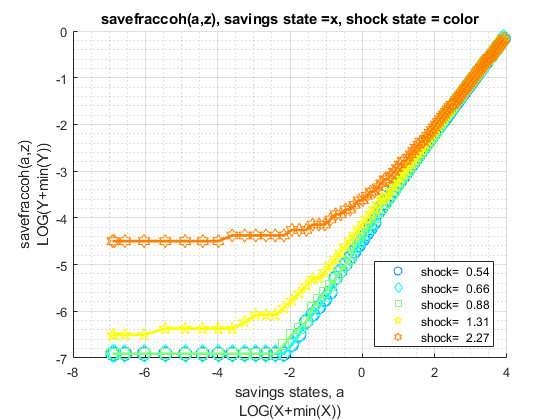
\includegraphics[width=5.20833in,height=\textheight]{img/fx_vfi_az_loop_images/figure_3.png}

When risk aversion increases, at every state-space point, the household
wants to save more.

\begin{verbatim}
% Higher Risk Aversion
mp_params('fl_crra') = 5;
ff_vfi_az_loop(mp_params, mp_support);

Elapsed time is 0.937495 seconds.
----------------------------------------
xxxxxxxxxxxxxxxxxxxxxxxxxxxxxxxxxxxxxxxx
CONTAINER NAME: mp_ffcmd ND Array (Matrix etc)
xxxxxxxxxxxxxxxxxxxxxxxxxxxxxxxxxxxxxxxx
                   i    idx    ndim    numel    rowN    colN     sum       mean        std      coefvari    min     max  
                   _    ___    ____    _____    ____    ____    ______    _______    _______    ________    ___    ______

    savefraccoh    1     1      2       500     100      5      335.64    0.67129    0.28688    0.42735      0     0.9488

xxx TABLE:savefraccoh xxxxxxxxxxxxxxxxxx
              c1         c2          c3         c4         c5   
            _______    _______    ________    _______    _______

    r1            0          0    0.078907    0.28472    0.52731
    r2            0          0    0.078904    0.28471     0.5273
    r3            0          0    0.078878    0.28465    0.52723
    r4            0          0    0.078808    0.28448    0.52705
    r5            0          0    0.078672    0.28415    0.52669
    r96     0.93086    0.92771     0.92215    0.94079    0.94593
    r97     0.93161    0.92855     0.92315    0.94183    0.94739
    r98     0.93233    0.92936     0.92411    0.94283     0.9488
    r99     0.93303    0.93015     0.92505    0.94379    0.92164
    r100    0.93371    0.93091     0.92595    0.94471    0.92317
\end{verbatim}

\includegraphics[width=5.20833in,height=\textheight]{img/fx_vfi_az_loop_images/figure_4.png}

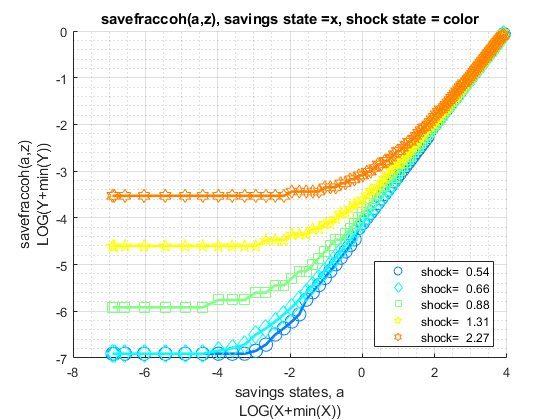
\includegraphics[width=5.20833in,height=\textheight]{img/fx_vfi_az_loop_images/figure_5.png}

\hypertarget{test-ff_vfi_az_loop-with-higher-uncertainty}{%
\subsection{Test FF\_VFI\_AZ\_LOOP with Higher Uncertainty}\label{test-ff_vfi_az_loop-with-higher-uncertainty}}

Increase the standard deviation of the Shock.

\begin{verbatim}
mp_support = containers.Map('KeyType','char', 'ValueType','any');
mp_support('bl_print_params') = false;
mp_support('bl_print_iterinfo') = false;
mp_support('ls_ffcmd') = {'savefraccoh'};
mp_support('ls_ffsna') = {};
mp_support('ls_ffgrh') = {};
mp_params = containers.Map('KeyType','char', 'ValueType','any');
mp_params('it_a_n') = 100;
mp_params('it_z_n') = 5;
mp_params('fl_a_max') = 50;
mp_params('st_grid_type') = 'grid_powerspace';
\end{verbatim}

Lower standard deviation of shock:

\begin{verbatim}
% Lower Risk Aversion
mp_params('fl_shk_std') = 0.10;
ff_vfi_az_loop(mp_params, mp_support);

Elapsed time is 0.957457 seconds.
----------------------------------------
xxxxxxxxxxxxxxxxxxxxxxxxxxxxxxxxxxxxxxxx
CONTAINER NAME: mp_ffcmd ND Array (Matrix etc)
xxxxxxxxxxxxxxxxxxxxxxxxxxxxxxxxxxxxxxxx
                   i    idx    ndim    numel    rowN    colN     sum      mean       std      coefvari    min      max  
                   _    ___    ____    _____    ____    ____    _____    ______    _______    ________    ___    _______

    savefraccoh    1     1      2       500     100      5      294.1    0.5882    0.32083    0.54544      0     0.92392

xxx TABLE:savefraccoh xxxxxxxxxxxxxxxxxx
              c1         c2         c3          c4         c5   
            _______    _______    _______    ________    _______

    r1            0          0          0    0.034556    0.11424
    r2            0          0          0    0.034555    0.11424
    r3            0          0          0    0.034546    0.11422
    r4            0          0          0    0.034523    0.11416
    r5            0          0          0    0.034478    0.11404
    r96     0.89673    0.89421    0.91986     0.91499    0.90808
    r97     0.89789    0.89545    0.92093      0.9162    0.90948
    r98     0.89903    0.89665    0.92196     0.91737    0.91084
    r99     0.90013    0.89782    0.92295      0.9185    0.91215
    r100    0.90119    0.89896    0.92392     0.91959    0.91342
\end{verbatim}

Higher shock standard deviation: low shock high asset save more, high
shock more asset save less, high shock low asset save more:

\begin{verbatim}
% Higher Risk Aversion
mp_params('fl_shk_std') = 0.40;
ff_vfi_az_loop(mp_params, mp_support);

Elapsed time is 0.923630 seconds.
----------------------------------------
xxxxxxxxxxxxxxxxxxxxxxxxxxxxxxxxxxxxxxxx
CONTAINER NAME: mp_ffcmd ND Array (Matrix etc)
xxxxxxxxxxxxxxxxxxxxxxxxxxxxxxxxxxxxxxxx
                   i    idx    ndim    numel    rowN    colN     sum       mean        std      coefvari    min      max  
                   _    ___    ____    _____    ____    ____    ______    _______    _______    ________    ___    _______

    savefraccoh    1     1      2       500     100      5      350.37    0.70073    0.26741    0.38162      0     0.93257

xxx TABLE:savefraccoh xxxxxxxxxxxxxxxxxx
              c1         c2          c3         c4         c5   
            _______    _______    ________    _______    _______

    r1            0          0    0.030722    0.36969    0.77072
    r2            0          0     0.03072    0.36967    0.77071
    r3            0          0      0.0307    0.36958    0.77068
    r4            0          0    0.030646    0.36933     0.7706
    r5            0          0    0.030543    0.36885    0.77044
    r96     0.90975    0.90819      0.9038    0.91513    0.88687
    r97     0.91053    0.90902     0.90476    0.91633    0.89076
    r98     0.91129    0.90982     0.90569     0.9175    0.86794
    r99     0.91204    0.91061      0.9066    0.91862    0.84583
    r100    0.91276    0.91138     0.90748    0.91971    0.82439
\end{verbatim}

\hypertarget{ff_vfi_az_vec-dynamic-savings-problem-vectorized-common-grid}{%
\section{FF\_VFI\_AZ\_VEC Dynamic Savings Problem Vectorized Common Grid}\label{ff_vfi_az_vec-dynamic-savings-problem-vectorized-common-grid}}

\begin{quote}
Go back to \href{http://fanwangecon.github.io/}{fan}'s \href{https://fanwangecon.github.io/MEconTools/}{MEconTools} Toolbox (\href{https://fanwangecon.github.io/MEconTools/bookdown}{bookdown}), \href{https://fanwangecon.github.io/M4Econ/}{Matlab Code Examples} Repository (\href{https://fanwangecon.github.io/M4Econ/bookdown}{bookdown}), or \href{https://fanwangecon.github.io/Math4Econ/}{Math for Econ with Matlab} Repository (\href{https://fanwangecon.github.io/Math4Econ/bookdown}{bookdown}).
\end{quote}

This is the example vignette for function:
\href{https://github.com/FanWangEcon/MEconTools/blob/master/MEconTools/vfi/ff_vfi_az_vec.m}{\textbf{ff\_vfi\_az\_vec}}
from the \href{https://fanwangecon.github.io/MEconTools/}{\textbf{MEconTools
Package}}\textbf{.} This function
solves (vectorized) the dynamic programming problem for a (a,z) model.
Households can save a, and face AR(1) shock z. The problem is solved
over the infinite horizon.

The code uses common grid, with the same state space and choice space
grids.
\href{https://github.com/FanWangEcon/MEconTools/blob/master/MEconTools/vfi/ff_vfi_az_bisec_vec.m}{\textbf{ff\_vfi\_az\_bisec\_vec}}
from the \href{https://fanwangecon.github.io/MEconTools/}{\textbf{MEconTools
Package}} solves the same
problem but using continuous exact percentage asset choices, which is
more precise than the solution here, and perhaps a little bit slower.

This is the vectorized code, its speed is much faster than the looped
code. The function is designed to have small memory footprint and
requires low computing resources, yet is fast.

\textbf{Links to Four Code:}

Four Core Savings/Borrowing Dynamic Programming Solution Functions that
are functions in the \href{https://fanwangecon.github.io/MEconTools/}{\textbf{MEconTools
Package}}\textbf{.} :

\begin{itemize}
\item
  Common Choice and States Grid :
  \href{https://github.com/FanWangEcon/MEconTools/blob/master/MEconTools/vfi/ff_vfi_az_loop.m}{\textbf{ff\_vfi\_az\_loop}},
  slow should use for testing new models
\item
  Common Choice and States Grid :
  \href{https://github.com/FanWangEcon/MEconTools/blob/master/MEconTools/vfi/ff_vfi_az_vec.m}{\textbf{ff\_vfi\_az\_vec}},
  fast good for many purposes
\item
  States Grid + Continuous Exact Savings as Share of Cash-on-Hand :\href{https://github.com/FanWangEcon/MEconTools/blob/master/MEconTools/vfi/ff_vfi_az_bisec_loop.m}{\textbf{ff\_vfi\_az\_bisec\_loop}},
  high precision even with small grid
\item
  States Grid + Continuous Exact Savings as Share of Cash-on-Hand :
  \href{https://github.com/FanWangEcon/MEconTools/blob/master/MEconTools/vfi/ff_vfi_az_bisec_vec.m}{\textbf{ff\_vfi\_az\_bisec\_vec}},
  precision and speed
\end{itemize}

\hypertarget{test-ff_vfi_az_vec-defaults}{%
\subsection{Test FF\_VFI\_AZ\_VEC Defaults}\label{test-ff_vfi_az_vec-defaults}}

Call the function with defaults. By default, shows the asset policy
function summary. Model parameters can be changed by the mp\_params.

\begin{verbatim}
%mp_params
mp_params = containers.Map('KeyType','char', 'ValueType','any');
mp_params('fl_crra') = 1.5;
mp_params('fl_beta') = 0.94;
ff_vfi_az_vec(mp_params);

Elapsed time is 0.128918 seconds.
----------------------------------------
xxxxxxxxxxxxxxxxxxxxxxxxxxxxxxxxxxxxxxxx
CONTAINER NAME: mp_ffcmd ND Array (Matrix etc)
xxxxxxxxxxxxxxxxxxxxxxxxxxxxxxxxxxxxxxxx
          i    idx    ndim    numel    rowN    colN     sum      mean      std     coefvari    min    max
          _    ___    ____    _____    ____    ____    _____    ______    _____    ________    ___    ___

    ap    1     1      2       700     100      7      16864    24.091    14.08    0.58446      0     50 

xxx TABLE:ap xxxxxxxxxxxxxxxxxx
              c1         c2         c3         c4         c5         c6         c7  
            _______    _______    _______    _______    _______    _______    ______

    r1            0          0          0          0          0    0.50505    2.0202
    r2            0          0          0    0.50505    0.50505     1.0101    2.5253
    r3      0.50505    0.50505    0.50505    0.50505     1.0101     1.5152    3.0303
    r4       1.0101     1.0101     1.0101     1.0101     1.5152     2.0202    3.5354
    r5       1.5152     1.5152     1.5152     1.5152     2.0202     2.5253    4.0404
    r96      45.455     45.455      45.96      45.96      45.96      46.97    48.485
    r97       45.96      45.96      45.96     46.465     46.465     47.475     48.99
    r98      46.465     46.465     46.465      46.97      46.97      47.98     48.99
    r99       46.97      46.97      46.97     47.475     47.475     48.485    49.495
    r100     47.475     47.475     47.475      47.98      47.98      48.99        50
\end{verbatim}

\hypertarget{test-ff_vfi_az_bisec_vec-speed-tests}{%
\subsection{Test FF\_VFI\_AZ\_BISEC\_VEC Speed Tests}\label{test-ff_vfi_az_bisec_vec-speed-tests}}

Call the function with different a and z grid size, print out speed:

\begin{verbatim}
mp_support = containers.Map('KeyType','char', 'ValueType','any');
mp_support('bl_timer') = true;
mp_support('ls_ffcmd') = {};
\end{verbatim}

A grid 200, shock grid 9:

\begin{verbatim}
mp_params = containers.Map('KeyType','char', 'ValueType','any');
mp_params('it_a_n') = 200;
mp_params('it_z_n') = 9;
ff_vfi_az_vec(mp_params, mp_support);

Elapsed time is 0.220867 seconds.
\end{verbatim}

A grid 750, shock grid 15:

\begin{verbatim}
mp_params = containers.Map('KeyType','char', 'ValueType','any');
mp_params('it_a_n') = 750;
mp_params('it_z_n') = 15;
ff_vfi_az_vec(mp_params, mp_support);

Elapsed time is 3.573648 seconds.
\end{verbatim}

A grid 600, shock grid 45:

\begin{verbatim}
mp_params = containers.Map('KeyType','char', 'ValueType','any');
mp_params('it_a_n') = 600;
mp_params('it_z_n') = 45;
ff_vfi_az_vec(mp_params, mp_support);

Elapsed time is 8.398580 seconds.
\end{verbatim}

\hypertarget{test-ff_vfi_az_vec-control-outputs}{%
\subsection{Test FF\_VFI\_AZ\_VEC Control Outputs}\label{test-ff_vfi_az_vec-control-outputs}}

Run the function first without any outputs;

\begin{verbatim}
mp_params = containers.Map('KeyType','char', 'ValueType','any');
mp_params('it_a_n') = 50;
mp_params('it_z_n') = 5;
mp_support = containers.Map('KeyType','char', 'ValueType','any');
mp_support('bl_timer') = false;
mp_support('bl_print_params') = false;
mp_support('bl_print_iterinfo') = false;
\end{verbatim}

Run the function and show policy function for savings choice. For
ls\_ffcmd, ls\_ffsna, ls\_ffgrh, can include these: `v', `ap', `c', `y',
`coh', `savefraccoh'. These are value, aprime savings choice,
consumption, income, cash on hand, and savings fraction as cash-on-hand.

\begin{verbatim}
mp_support = containers.Map('KeyType','char', 'ValueType','any');
mp_support('bl_print_params') = false;
mp_support('bl_print_iterinfo') = false;
% ls_ffcmd: summary print which outcomes
mp_support('ls_ffcmd') = {};
% ls_ffsna: detail print which outcomes
mp_support('ls_ffsna') = {'savefraccoh'};
% ls_ffgrh: graphical print which outcomes
mp_support('ls_ffgrh') = {'savefraccoh'};
ff_vfi_az_vec(mp_params, mp_support);

Elapsed time is 0.014484 seconds.
xxx  ff_vfi_az_vec, outcome=savefraccoh  xxxxxxxxxxxxxxxxxxxxxxxxxxx
    group      a       mean_z_0_54195    mean_z_0_66401    mean_z_0_88162    mean_z_1_3095    mean_z_2_2745
    _____    ______    ______________    ______________    ______________    _____________    _____________

      1           0             0                 0                 0                 0           0.3505   
      2      1.0204             0                 0           0.46928           0.37487          0.51572   
      3      2.0408       0.36632           0.34687           0.63373           0.54163          0.61186   
      4      3.0612       0.53265           0.51178           0.47837           0.63592          0.67476   
      5      4.0816       0.62764           0.60816           0.57627           0.69655          0.71911   
      6       5.102       0.68908           0.67137           0.64196           0.73882          0.75206   
      7      6.1224       0.73208           0.71603           0.68909           0.76996          0.77751   
      8      7.1429       0.76386           0.74926           0.72456           0.79387          0.79776   
      9      8.1633        0.7883           0.77494           0.75221           0.81279          0.81425   
     10      9.1837       0.80769           0.79539           0.77438           0.82815          0.82795   
     11      10.204       0.82343           0.81206           0.79254           0.84086           0.8395   
     12      11.224       0.83648           0.82591            0.8077           0.85155          0.84937   
     13      12.245       0.84747           0.83759           0.82053           0.86067          0.85791   
     14      13.265       0.85685           0.84758           0.83155           0.80173          0.86537   
     15      14.286       0.86495           0.85622            0.8411           0.81288          0.87194   
     16      15.306       0.87201           0.86377           0.84947           0.82268          0.82291   
     17      16.327       0.87823           0.87043           0.85685           0.83137          0.83104   
     18      17.347       0.88374           0.87633           0.86342           0.83912          0.83834   
     19      18.367       0.88866           0.88161            0.8693           0.84608          0.84495   
     20      19.388       0.89309           0.88635            0.8746           0.85237          0.85095   
     21      20.408       0.89708           0.89064           0.87939           0.85807          0.85642   
     22      21.429       0.85567           0.89454           0.88375           0.86327          0.86143   
     23      22.449       0.86096           0.89809           0.88773           0.86803          0.86604   
     24      23.469       0.86581           0.90135           0.89138           0.87241          0.87029   
     25       24.49       0.87026           0.86502           0.89474           0.87644          0.87422   
     26       25.51       0.87436            0.8693           0.89784           0.88017          0.87787   
     27      26.531       0.87816           0.87327           0.90071           0.88362          0.88126   
     28      27.551       0.88168           0.87695           0.90338           0.88684          0.88443   
     29      28.571       0.88496           0.88037           0.90586           0.88984          0.88739   
     30      29.592       0.88802           0.88357           0.90818           0.89264          0.89017   
     31      30.612       0.89087           0.88655           0.87896           0.89527          0.89278   
     32      31.633       0.89355           0.88935           0.88197           0.89773          0.89523   
     33      32.653       0.89606           0.89198            0.8848           0.90005          0.89754   
     34      33.673       0.89843           0.89446           0.88747           0.90223          0.89972   
     35      34.694       0.90065           0.89679           0.88998           0.90429          0.90178   
     36      35.714       0.90275           0.89899           0.89235           0.90624          0.90374   
     37      36.735       0.90474           0.90107            0.8946           0.90809          0.90559   
     38      37.755       0.90662           0.90304           0.89673           0.90984          0.90735   
     39      38.776       0.90841           0.90491           0.89874            0.9115          0.90902   
     40      39.796        0.9101           0.90669           0.90066           0.91308          0.91062   
     41      40.816       0.91171           0.90838           0.90249           0.91458          0.91214   
     42      41.837       0.91325           0.90998           0.90422           0.91601          0.91359   
     43      42.857       0.91471           0.91152           0.90588           0.91738          0.91497   
     44      43.878        0.9161           0.91298           0.90746           0.89681          0.89499   
     45      44.898       0.91743           0.91438           0.90897           0.89854          0.89671   
     46      45.918       0.91871           0.91571           0.91042           0.90019          0.89836   
     47      46.939       0.91993           0.91699           0.91181           0.90178          0.89994   
     48      47.959        0.9211           0.91822           0.91313            0.9033          0.90146   
     49       48.98       0.92222           0.91939           0.91441           0.90475          0.90292   
     50          50       0.92329           0.92052           0.91563           0.90615          0.90433   
\end{verbatim}

\includegraphics[width=5.20833in,height=\textheight]{img/fx_vfi_az_vec_images/figure_0.png}

\includegraphics[width=5.20833in,height=\textheight]{img/fx_vfi_az_vec_images/figure_1.png}

Run the function and show summaries for savings and fraction of coh
saved:

\begin{verbatim}
mp_params('it_a_n') = 100;
mp_params('it_z_n') = 9;
mp_support('ls_ffcmd') = {'ap', 'savefraccoh'};
mp_support('ls_ffsna') = {};
mp_support('ls_ffgrh') = {};
mp_support('bl_vfi_store_all') = true; % store c(a,z), y(a,z)
ff_vfi_az_vec(mp_params, mp_support);

Elapsed time is 0.127807 seconds.
----------------------------------------
xxxxxxxxxxxxxxxxxxxxxxxxxxxxxxxxxxxxxxxx
CONTAINER NAME: mp_ffcmd ND Array (Matrix etc)
xxxxxxxxxxxxxxxxxxxxxxxxxxxxxxxxxxxxxxxx
                   i    idx    ndim    numel    rowN    colN     sum       mean        std      coefvari    min      max  
                   _    ___    ____    _____    ____    ____    ______    _______    _______    ________    ___    _______

    ap             1     1      2       900     100      9       21825      24.25     14.089      0.581      0          50
    savefraccoh    2     2      2       900     100      9      752.38    0.83597    0.13497    0.16145      0     0.91812

xxx TABLE:ap xxxxxxxxxxxxxxxxxx
              c1         c2         c3         c4         c5         c6         c7         c8        c9  
            _______    _______    _______    _______    _______    _______    _______    ______    ______

    r1            0          0          0          0          0          0    0.50505    1.5152    3.0303
    r2            0          0          0          0    0.50505    0.50505     1.0101    1.5152    3.5354
    r3      0.50505    0.50505    0.50505    0.50505    0.50505     1.0101     1.5152    2.0202    4.0404
    r4       1.0101     1.0101     1.0101     1.0101     1.0101     1.5152     2.0202    2.5253    4.5455
    r5       1.5152     1.5152     1.5152     1.5152     1.5152     2.0202     2.5253    3.0303    5.0505
    r96      45.455     45.455     45.455      45.96      45.96      45.96     46.465    47.475    49.495
    r97       45.96      45.96      45.96     46.465     46.465     46.465      46.97     47.98    49.495
    r98      46.465     46.465     46.465     46.465      46.97      46.97     47.475    48.485        50
    r99       46.97      46.97      46.97      46.97     47.475     47.475      47.98     48.99        50
    r100     47.475     47.475     47.475     47.475      47.98      47.98     48.485    49.495        50

xxx TABLE:savefraccoh xxxxxxxxxxxxxxxxxx
              c1         c2         c3         c4         c5         c6         c7         c8         c9   
            _______    _______    _______    _______    _______    _______    _______    _______    _______

    r1            0          0          0          0          0          0    0.24587    0.48182    0.56208
    r2            0          0          0          0     0.3075    0.25444    0.39276    0.41371    0.59831
    r3      0.30679    0.29486    0.27938    0.25939     0.2338    0.40362    0.49043     0.4833     0.6287
    r4       0.4668    0.45285    0.43438    0.40981    0.37721    0.50166    0.56006    0.53755    0.65456
    r5      0.56502    0.55132    0.53293    0.50802    0.47415    0.57101    0.61221    0.58103    0.67683
    r96     0.91292     0.9117    0.90997    0.91752    0.91364    0.90746    0.90692    0.90732    0.90699
    r97     0.91357    0.91236    0.91064    0.91812    0.91427    0.90815    0.90761    0.90799    0.89847
    r98      0.9142      0.913     0.9113    0.90882    0.91489    0.90882    0.90828    0.90865    0.89919
    r99     0.91482    0.91363    0.91195    0.90949    0.91549    0.90949    0.90894    0.90929    0.89089
    r100    0.91543    0.91425    0.91258    0.91014    0.91609    0.91013    0.90959    0.90992    0.88275
\end{verbatim}

\hypertarget{test-ff_vfi_az_vec-change-interest-rate-and-discount}{%
\subsection{Test FF\_VFI\_AZ\_VEC Change Interest Rate and Discount}\label{test-ff_vfi_az_vec-change-interest-rate-and-discount}}

Show only save fraction of cash on hand:

\begin{verbatim}
mp_support = containers.Map('KeyType','char', 'ValueType','any');
mp_support('bl_print_params') = false;
mp_support('bl_print_iterinfo') = false;
mp_support('ls_ffcmd') = {'savefraccoh'};
mp_support('ls_ffsna') = {};
mp_support('ls_ffgrh') = {};
mp_params = containers.Map('KeyType','char', 'ValueType','any');
mp_params('it_a_n') = 750;
mp_params('it_z_n') = 9;
mp_params('fl_a_max') = 50;
mp_params('st_grid_type') = 'grid_powerspace';
\end{verbatim}

Solve the model with several different interest rates and discount
factor:

\begin{verbatim}
% Lower Savings Incentives
mp_params('fl_beta') = 0.80;
mp_params('fl_r') = 0.01;
ff_vfi_az_vec(mp_params, mp_support);

Elapsed time is 0.771613 seconds.
----------------------------------------
xxxxxxxxxxxxxxxxxxxxxxxxxxxxxxxxxxxxxxxx
CONTAINER NAME: mp_ffcmd ND Array (Matrix etc)
xxxxxxxxxxxxxxxxxxxxxxxxxxxxxxxxxxxxxxxx
                   i    idx    ndim    numel    rowN    colN     sum       mean        std      coefvari    min      max  
                   _    ___    ____    _____    ____    ____    ______    _______    _______    ________    ___    _______

    savefraccoh    1     1      2      6750     750      9      3318.8    0.49167    0.27768    0.56477      0     0.80542

xxx TABLE:savefraccoh xxxxxxxxxxxxxxxxxx
              c1         c2         c3         c4         c5         c6          c7         c8         c9   
            _______    _______    _______    _______    _______    _______    ________    _______    _______

    r1            0          0          0          0          0          0    0.023475    0.13289    0.29755
    r2            0          0          0          0          0          0    0.023475    0.13289    0.29755
    r3            0          0          0          0          0          0    0.023475    0.13289    0.29755
    r4            0          0          0          0          0          0    0.023475    0.13289    0.29755
    r5            0          0          0          0          0          0    0.023475    0.13289    0.29755
    r746     0.8044    0.80333    0.80182    0.79961    0.79626    0.79093      0.7887     0.7824    0.77641
    r747    0.80465    0.80359    0.80209    0.79989    0.79655    0.79124     0.78903    0.78277    0.77686
    r748    0.80491    0.80385    0.80235    0.80016    0.79683    0.79154     0.78936    0.78315    0.77731
    r749    0.80517    0.80411    0.80262    0.80043    0.79712    0.79185     0.78969    0.78352    0.77776
    r750    0.80542    0.80437    0.80288    0.80071     0.7974    0.79215     0.79002    0.78389    0.77821

% Higher Savings Incentives
mp_params('fl_beta') = 0.95;
mp_params('fl_r') = 0.04;
ff_vfi_az_vec(mp_params, mp_support);

Elapsed time is 2.484993 seconds.
----------------------------------------
xxxxxxxxxxxxxxxxxxxxxxxxxxxxxxxxxxxxxxxx
CONTAINER NAME: mp_ffcmd ND Array (Matrix etc)
xxxxxxxxxxxxxxxxxxxxxxxxxxxxxxxxxxxxxxxx
                   i    idx    ndim    numel    rowN    colN     sum       mean        std      coefvari    min      max  
                   _    ___    ____    _____    ____    ____    ______    _______    _______    ________    ___    _______

    savefraccoh    1     1      2      6750     750      9      4491.9    0.66547    0.28771    0.43234      0     0.93029

xxx TABLE:savefraccoh xxxxxxxxxxxxxxxxxx
              c1         c2         c3         c4          c5         c6         c7         c8         c9   
            _______    _______    _______    _______    ________    _______    _______    _______    _______

    r1            0          0          0          0    0.031818    0.14726    0.31047    0.48484    0.64489
    r2            0          0          0          0    0.031818    0.14726    0.31047    0.48484    0.64489
    r3            0          0          0          0    0.031818    0.14726    0.31047    0.48484    0.64489
    r4            0          0          0          0    0.031818    0.14726    0.31047    0.48484    0.64489
    r5            0          0          0          0    0.031818    0.14726    0.31047    0.48484    0.64489
    r746    0.92742       0.93     0.9283    0.92581     0.92578    0.92349    0.92443    0.91686    0.88398
    r747     0.9275    0.93007    0.92838     0.9259     0.92588    0.92361    0.92457    0.91706    0.88076
    r748    0.92757    0.93014    0.92846    0.92599     0.92598    0.92373    0.92472    0.91359    0.87757
    r749    0.92764    0.93022    0.92854    0.92608     0.92608    0.92384    0.92115    0.91014    0.87438
    r750    0.92772    0.93029    0.92862    0.92617     0.92618    0.92396     0.9213    0.90671    0.87121
\end{verbatim}

\hypertarget{test-ff_vfi_az_vec-changing-risk-aversion}{%
\subsection{Test FF\_VFI\_AZ\_VEC Changing Risk Aversion}\label{test-ff_vfi_az_vec-changing-risk-aversion}}

Here, again, show fraction of coh saved in summary tabular form, but
also show it graphically.

\begin{verbatim}
mp_support = containers.Map('KeyType','char', 'ValueType','any');
mp_support('bl_print_params') = false;
mp_support('bl_print_iterinfo') = false;
mp_support('ls_ffcmd') = {'savefraccoh'};
mp_support('ls_ffsna') = {};
mp_support('ls_ffgrh') = {'savefraccoh'};
mp_params = containers.Map('KeyType','char', 'ValueType','any');
mp_params('it_a_n') = 750;
mp_params('it_z_n') = 9;
mp_params('fl_a_max') = 50;
mp_params('st_grid_type') = 'grid_powerspace';
\end{verbatim}

Solve the model with different risk aversion levels, higher preferences
for risk:

\begin{verbatim}
% Lower Risk Aversion
mp_params('fl_crra') = 0.5;
ff_vfi_az_vec(mp_params, mp_support);

Elapsed time is 1.991475 seconds.
----------------------------------------
xxxxxxxxxxxxxxxxxxxxxxxxxxxxxxxxxxxxxxxx
CONTAINER NAME: mp_ffcmd ND Array (Matrix etc)
xxxxxxxxxxxxxxxxxxxxxxxxxxxxxxxxxxxxxxxx
                   i    idx    ndim    numel    rowN    colN     sum       mean       std      coefvari    min      max  
                   _    ___    ____    _____    ____    ____    ______    _______    ______    ________    ___    _______

    savefraccoh    1     1      2      6750     750      9      3735.9    0.55347    0.2897    0.52343      0     0.85998

xxx TABLE:savefraccoh xxxxxxxxxxxxxxxxxx
              c1         c2         c3         c4         c5         c6          c7         c8         c9   
            _______    _______    _______    _______    _______    _______    ________    _______    _______

    r1            0          0          0          0          0          0    0.075021    0.22812    0.41075
    r2            0          0          0          0          0          0    0.075021    0.22812    0.41075
    r3            0          0          0          0          0          0    0.075021    0.22812    0.41075
    r4            0          0          0          0          0          0    0.075021    0.22812    0.41075
    r5            0          0          0          0          0          0    0.075021    0.22812    0.41075
    r746    0.85928    0.85816    0.85657    0.85425    0.85428     0.8522     0.84972    0.84635    0.84292
    r747    0.85946    0.85834    0.85676    0.85444    0.85449    0.85242     0.84997    0.84665     0.8433
    r748    0.85963    0.85852    0.85694    0.85464    0.85469    0.85264     0.85021    0.84694    0.84368
    r749    0.85981     0.8587    0.85713    0.85483    0.85489    0.85286     0.85046    0.84723    0.84405
    r750    0.85998    0.85888    0.85731    0.85502    0.85509    0.85307      0.8507    0.84752    0.84442
\end{verbatim}

\includegraphics[width=5.20833in,height=\textheight]{img/fx_vfi_az_vec_images/figure_2.png}

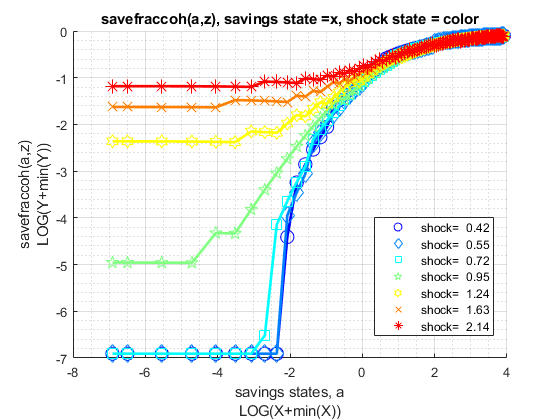
\includegraphics[width=5.20833in,height=\textheight]{img/fx_vfi_az_vec_images/figure_3.png}

When risk aversion increases, at every state-space point, the household
wants to save more.

\begin{verbatim}
% Higher Risk Aversion
mp_params('fl_crra') = 5;
ff_vfi_az_vec(mp_params, mp_support);

Elapsed time is 2.026442 seconds.
----------------------------------------
xxxxxxxxxxxxxxxxxxxxxxxxxxxxxxxxxxxxxxxx
CONTAINER NAME: mp_ffcmd ND Array (Matrix etc)
xxxxxxxxxxxxxxxxxxxxxxxxxxxxxxxxxxxxxxxx
                   i    idx    ndim    numel    rowN    colN     sum       mean       std      coefvari    min     max 
                   _    ___    ____    _____    ____    ____    ______    ______    _______    ________    ___    _____

    savefraccoh    1     1      2      6750     750      9      4639.3    0.6873    0.28204    0.41036      0     0.942

xxx TABLE:savefraccoh xxxxxxxxxxxxxxxxxx
              c1         c2         c3          c4           c5         c6         c7         c8         c9   
            _______    _______    _______    _________    ________    _______    _______    _______    _______

    r1            0          0          0     0.008995    0.085095    0.21314    0.37277    0.53628    0.68332
    r2            0          0          0     0.008995    0.085095    0.21314    0.37277    0.53628    0.68332
    r3            0          0          0     0.008995    0.085095    0.21314    0.37277    0.53628    0.68332
    r4            0          0          0     0.008995    0.085095    0.21314    0.37277    0.53628    0.68332
    r5            0          0          0    0.0089949    0.085094    0.21314    0.37277    0.53628    0.68332
    r746    0.94083     0.9396    0.94168      0.93912     0.93904    0.94041    0.93743    0.92949    0.89566
    r747    0.94091    0.93969    0.94176      0.93921     0.93914    0.93674    0.93758    0.92969    0.89241
    r748    0.94098    0.93977    0.94184      0.93931     0.93924    0.93686    0.93772    0.92618    0.88918
    r749    0.94106    0.93985    0.94192       0.9394     0.93934    0.93699    0.93787    0.92269    0.88596
    r750    0.94113    0.93993      0.942      0.93949     0.93944    0.93711    0.93801    0.91921    0.88275
\end{verbatim}

\includegraphics[width=5.20833in,height=\textheight]{img/fx_vfi_az_vec_images/figure_4.png}

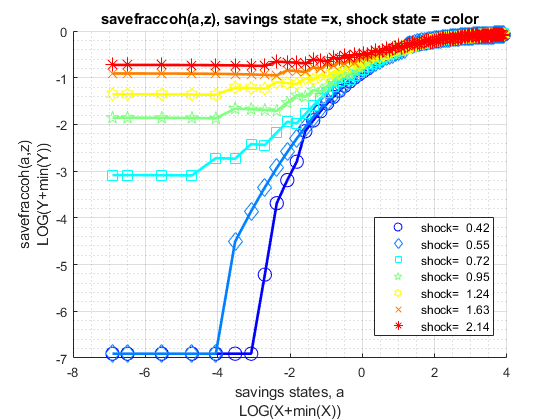
\includegraphics[width=5.20833in,height=\textheight]{img/fx_vfi_az_vec_images/figure_5.png}

\hypertarget{test-ff_vfi_az_vec-with-higher-uncertainty}{%
\subsection{Test FF\_VFI\_AZ\_VEC with Higher Uncertainty}\label{test-ff_vfi_az_vec-with-higher-uncertainty}}

Increase the standard deviation of the Shock.

\begin{verbatim}
mp_support = containers.Map('KeyType','char', 'ValueType','any');
mp_support('bl_print_params') = false;
mp_support('bl_print_iterinfo') = false;
mp_support('ls_ffcmd') = {'savefraccoh'};
mp_support('ls_ffsna') = {};
mp_support('ls_ffgrh') = {};
mp_params = containers.Map('KeyType','char', 'ValueType','any');
mp_params('it_a_n') = 750;
mp_params('it_z_n') = 9;
mp_params('fl_a_max') = 50;
mp_params('st_grid_type') = 'grid_powerspace';
\end{verbatim}

Lower standard deviation of shock:

\begin{verbatim}
% Lower Risk Aversion
mp_params('fl_shk_std') = 0.10;
ff_vfi_az_vec(mp_params, mp_support);

Elapsed time is 2.065989 seconds.
----------------------------------------
xxxxxxxxxxxxxxxxxxxxxxxxxxxxxxxxxxxxxxxx
CONTAINER NAME: mp_ffcmd ND Array (Matrix etc)
xxxxxxxxxxxxxxxxxxxxxxxxxxxxxxxxxxxxxxxx
                   i    idx    ndim    numel    rowN    colN    sum      mean        std      coefvari    min      max  
                   _    ___    ____    _____    ____    ____    ____    _______    _______    ________    ___    _______

    savefraccoh    1     1      2      6750     750      9      4026    0.59644    0.31533    0.52869      0     0.91423

xxx TABLE:savefraccoh xxxxxxxxxxxxxxxxxx
              c1         c2         c3         c4         c5          c6          c7         c8         c9   
            _______    _______    _______    _______    _______    ________    ________    _______    _______

    r1            0          0          0          0          0    0.012569    0.062884    0.13754    0.22274
    r2            0          0          0          0          0    0.012569    0.062884    0.13754    0.22274
    r3            0          0          0          0          0    0.012569    0.062884    0.13754    0.22274
    r4            0          0          0          0          0    0.012569    0.062884    0.13754    0.22274
    r5            0          0          0          0          0    0.012569    0.062884    0.13754    0.22274
    r746    0.91375    0.91251    0.91101    0.91289    0.91057     0.91138     0.91136    0.91021     0.9075
    r747    0.91387    0.91264    0.91114    0.91302    0.91072     0.91153     0.91152    0.91039    0.90769
    r748    0.91399    0.91277    0.91127    0.91315    0.91086     0.91168     0.91168    0.91056    0.90788
    r749    0.91411    0.91289     0.9114    0.91329      0.911     0.91183     0.91183    0.91073    0.90807
    r750    0.91423    0.91302    0.91153    0.91342    0.91114     0.91197     0.91199     0.9109    0.90826
\end{verbatim}

Higher shock standard deviation: low shock high asset save more, high
shock more asset save less, high shock low asset save more:

\begin{verbatim}
% Higher Risk Aversion
mp_params('fl_shk_std') = 0.40;
ff_vfi_az_vec(mp_params, mp_support);

Elapsed time is 2.184888 seconds.
----------------------------------------
xxxxxxxxxxxxxxxxxxxxxxxxxxxxxxxxxxxxxxxx
CONTAINER NAME: mp_ffcmd ND Array (Matrix etc)
xxxxxxxxxxxxxxxxxxxxxxxxxxxxxxxxxxxxxxxx
                   i    idx    ndim    numel    rowN    colN     sum       mean        std      coefvari    min     max  
                   _    ___    ____    _____    ____    ____    ______    _______    _______    ________    ___    ______

    savefraccoh    1     1      2      6750     750      9      4687.4    0.69442    0.27109    0.39038      0     0.9339

xxx TABLE:savefraccoh xxxxxxxxxxxxxxxxxx
              c1         c2         c3         c4          c5         c6         c7         c8         c9   
            _______    _______    _______    _______    ________    _______    _______    _______    _______

    r1            0          0          0          0    0.030619    0.24561    0.55369    0.80189    0.46265
    r2            0          0          0          0    0.030619    0.24561    0.55369    0.80189    0.46265
    r3            0          0          0          0    0.030619     0.2456    0.55369    0.80189    0.46265
    r4            0          0          0          0    0.030619     0.2456    0.55369    0.80189    0.46265
    r5            0          0          0          0    0.030618     0.2456    0.55369    0.80189    0.46265
    r746    0.93365    0.93335     0.9328    0.93173     0.92941    0.92713    0.92079     0.8402    0.31544
    r747    0.93371    0.93341    0.93286     0.9318     0.92949    0.92723    0.92095    0.83734    0.31504
    r748    0.93378    0.93348    0.93293    0.93187     0.92957    0.92733    0.92111    0.83449    0.31463
    r749    0.93384    0.93354      0.933    0.93194     0.92965    0.92743    0.92127    0.83166    0.31423
    r750     0.9339     0.9336    0.93306    0.93201     0.92973    0.92753    0.92143    0.82883    0.31383
\end{verbatim}

\hypertarget{ff_vfi_az_bisec_loop-dynamic-savings-problem-loop-continuous-choice}{%
\section{FF\_VFI\_AZ\_BISEC\_LOOP Dynamic Savings Problem Loop Continuous Choice}\label{ff_vfi_az_bisec_loop-dynamic-savings-problem-loop-continuous-choice}}

\begin{quote}
Go back to \href{http://fanwangecon.github.io/}{fan}'s \href{https://fanwangecon.github.io/MEconTools/}{MEconTools} Toolbox (\href{https://fanwangecon.github.io/MEconTools/bookdown}{bookdown}), \href{https://fanwangecon.github.io/M4Econ/}{Matlab Code Examples} Repository (\href{https://fanwangecon.github.io/M4Econ/bookdown}{bookdown}), or \href{https://fanwangecon.github.io/Math4Econ/}{Math for Econ with Matlab} Repository (\href{https://fanwangecon.github.io/Math4Econ/bookdown}{bookdown}).
\end{quote}

This is the example vignette for function:\href{https://github.com/FanWangEcon/MEconTools/blob/master/MEconTools/vfi/ff_vfi_az_bisec_loop.m}{\textbf{ff\_vfi\_az\_bisec\_loop}}from
the \href{https://fanwangecon.github.io/MEconTools/}{\textbf{MEconTools
Package}}\textbf{.} This function
solves the dynamic programming problem for a (a,z) model. Households can
save (face some borrowing constraint), and face AR(1) shock z. The
problem is solved over the infinite horizon. This is the looped code, it
is slow for larger state-space problems. The code uses continuous
choices, solved with bisection. The state-space is on a grid, but choice
grids are in terms of percentage of resources to save and solved
exactly.

\textbf{Links to Four Code:}

Four Core Savings/Borrowing Dynamic Programming Solution Functions that
are functions in the \href{https://fanwangecon.github.io/MEconTools/}{\textbf{MEconTools
Package}}\textbf{.} :

\begin{itemize}
\item
  Common Choice and States Grid :
  \href{https://github.com/FanWangEcon/MEconTools/blob/master/MEconTools/vfi/ff_vfi_az_loop.m}{\textbf{ff\_vfi\_az\_loop}},
  slow should use for testing new models
\item
  Common Choice and States Grid :
  \href{https://github.com/FanWangEcon/MEconTools/blob/master/MEconTools/vfi/ff_vfi_az_vec.m}{\textbf{ff\_vfi\_az\_vec}},
  fast good for many purposes
\item
  States Grid + Continuous Exact Savings as Share of Cash-on-Hand :\href{https://github.com/FanWangEcon/MEconTools/blob/master/MEconTools/vfi/ff_vfi_az_bisec_loop.m}{\textbf{ff\_vfi\_az\_bisec\_loop}},
  high precision even with small grid
\item
  States Grid + Continuous Exact Savings as Share of Cash-on-Hand :
  \href{https://github.com/FanWangEcon/MEconTools/blob/master/MEconTools/vfi/ff_vfi_az_bisec_vec.m}{\textbf{ff\_vfi\_az\_bisec\_vec}},
  precision and speed
\end{itemize}

\hypertarget{test-ff_vfi_az_bisec_loop-defaults}{%
\subsection{Test FF\_VFI\_AZ\_BISEC\_LOOP Defaults}\label{test-ff_vfi_az_bisec_loop-defaults}}

Call the function with defaults. By default, shows the asset policy
function summary. Model parameters can be changed by the mp\_params.

\begin{verbatim}
%mp_params
mp_params = containers.Map('KeyType','char', 'ValueType','any');
mp_params('fl_crra') = 1.5;
mp_params('fl_beta') = 0.94;
% call function
ff_vfi_az_bisec_loop(mp_params);

Elapsed time is 31.520504 seconds.
----------------------------------------
xxxxxxxxxxxxxxxxxxxxxxxxxxxxxxxxxxxxxxxx
CONTAINER NAME: mp_ffcmd ND Array (Matrix etc)
xxxxxxxxxxxxxxxxxxxxxxxxxxxxxxxxxxxxxxxx
          i    idx    ndim    numel    rowN    colN     sum      mean      std      coefvari    min     max  
          _    ___    ____    _____    ____    ____    _____    ______    ______    ________    ___    ______

    ap    1     1      2       700     100      7      16866    24.094    14.071    0.58399      0     50.252

xxx TABLE:ap xxxxxxxxxxxxxxxxxx
              c1         c2         c3         c4         c5         c6         c7  
            _______    _______    _______    _______    _______    _______    ______

    r1            0          0          0          0    0.13188    0.66203    1.9859
    r2      0.25914    0.26426    0.29511    0.39221    0.57697     1.1208    2.4569
    r3      0.65371    0.66543    0.70966    0.82502      1.029      1.582    2.9298
    r4       1.0748     1.0921     1.1447     1.2698     1.5151     2.0481    3.4046
    r5       1.5152     1.5319     1.5903      1.721     2.0011     2.5252    3.8802
    r96      45.561     45.615     45.712     45.887     46.192     46.835    48.252
    r97      46.049     46.104     46.201     46.377     46.681     47.325    48.743
    r98       46.54     46.593      46.69     46.866     47.171     47.815    49.235
    r99      47.029     47.082     47.179     47.356     47.661     48.304    49.734
    r100     47.518     47.572      47.67     47.845      48.15     48.793    50.252
\end{verbatim}

\hypertarget{test-ff_vfi_az_bisec_loop-speed-tests}{%
\subsection{Test FF\_VFI\_AZ\_BISEC\_LOOP Speed Tests}\label{test-ff_vfi_az_bisec_loop-speed-tests}}

Call the function with different a and z grid size, print out speed:

\begin{verbatim}
mp_support = containers.Map('KeyType','char', 'ValueType','any');
mp_support('bl_timer') = true;
mp_support('ls_ffcmd') = {};
\end{verbatim}

A grid 50, shock grid 5:

\begin{verbatim}
mp_params = containers.Map('KeyType','char', 'ValueType','any');
mp_params('it_a_n') = 50;
mp_params('it_z_n') = 5;
ff_vfi_az_bisec_loop(mp_params, mp_support);

Elapsed time is 9.142315 seconds.
\end{verbatim}

A grid 100, shock grid 7:

\begin{verbatim}
mp_params = containers.Map('KeyType','char', 'ValueType','any');
mp_params('it_a_n') = 100;
mp_params('it_z_n') = 7;
ff_vfi_az_bisec_loop(mp_params, mp_support);

Elapsed time is 26.910198 seconds.
\end{verbatim}

A grid 200, shock grid 9:

\begin{verbatim}
mp_params = containers.Map('KeyType','char', 'ValueType','any');
mp_params('it_a_n') = 200;
mp_params('it_z_n') = 9;
ff_vfi_az_bisec_loop(mp_params, mp_support);

Elapsed time is 74.127079 seconds.
\end{verbatim}

\hypertarget{test-ff_vfi_az_bisec_loop-control-outputs}{%
\subsection{Test FF\_VFI\_AZ\_BISEC\_LOOP Control Outputs}\label{test-ff_vfi_az_bisec_loop-control-outputs}}

Run the function first without any outputs;

\begin{verbatim}
mp_params = containers.Map('KeyType','char', 'ValueType','any');
mp_params('it_a_n') = 50;
mp_params('it_z_n') = 5;
mp_support = containers.Map('KeyType','char', 'ValueType','any');
mp_support('bl_timer') = false;
mp_support('bl_print_params') = false;
mp_support('bl_print_iterinfo') = false;
\end{verbatim}

Run the function and show policy function for savings choice. For
ls\_ffcmd, ls\_ffsna, ls\_ffgrh, can include these: `v', `ap', `c', `y',
`coh', `savefraccoh'. These are value, aprime savings choice,
consumption, income, cash on hand, and savings fraction as cash-on-hand.

\begin{verbatim}
mp_support = containers.Map('KeyType','char', 'ValueType','any');
mp_support('bl_print_params') = false;
mp_support('bl_print_iterinfo') = false;
% ls_ffcmd: summary print which outcomes
mp_support('ls_ffcmd') = {};
% ls_ffsna: detail print which outcomes
mp_support('ls_ffsna') = {'ap'};
% ls_ffgrh: graphical print which outcomes
mp_support('ls_ffgrh') = {'ap'};
ff_vfi_az_bisec_loop(mp_params, mp_support);

Elapsed time is 9.221215 seconds.
xxx  ff_vfi_az_vec, outcome=ap  xxxxxxxxxxxxxxxxxxxxxxxxxxx
    group      a       mean_z_0_54195    mean_z_0_66401    mean_z_0_88162    mean_z_1_3095    mean_z_2_2745
    _____    ______    ______________    ______________    ______________    _____________    _____________

      1           0             0                 0                 0           0.17037          1.0635    
      2      1.0204       0.69295           0.72405           0.84423             1.099          2.0409    
      3      2.0408        1.5665            1.6143            1.7589            2.0408          3.0571    
      4      3.0612        2.4757             2.534            2.6903            3.0612          4.0135    
      5      4.0816        3.4036            3.4686            3.6319            4.0274          4.9775    
      6       5.102        4.3431            4.4131            4.5822            4.9848          5.9445    
      7      6.1224        5.2908            5.3648            5.5384            5.9466          6.9138    
      8      7.1429        6.2445            6.3216            6.4989            6.9116          7.8851    
      9      8.1633        7.2029            7.2827             7.463            7.8793          8.8584    
     10      9.1837        8.1651            8.2469            8.4301            8.8495          9.8329    
     11      10.204        9.1837            9.2139            9.3992            9.8212          10.809    
     12      11.224        10.175            10.204             10.37            10.795          11.785    
     13      12.245        11.141            11.225            11.343            11.769          12.763    
     14      13.265        12.109            12.198            12.316            12.745          13.742    
     15      14.286        13.079            13.169            13.291            13.721           14.72    
     16      15.306        14.051            14.142            14.286            14.699            15.7    
     17      16.327        15.026            15.117            15.306            15.677           16.68    
     18      17.347        16.001            16.093            16.289            16.655           17.66    
     19      18.367        16.978            17.069            17.265            17.634          18.641    
     20      19.388        17.955            18.048            18.243            18.614          19.623    
     21      20.408        18.934            19.026            19.223            19.595          20.606    
     22      21.429        19.913            20.006            20.203            20.577          21.589    
     23      22.449        20.894            20.986            21.184            21.559          22.573    
     24      23.469        21.875            21.968            22.166            22.542          23.557    
     25       24.49        22.856             22.95            23.148            23.525          24.542    
     26       25.51        23.838            23.932            24.131            24.509          25.526    
     27      26.531        24.821            24.915            25.114             25.51          26.531    
     28      27.551        25.804            25.899            26.098            26.531          27.551    
     29      28.571        26.788            26.883            27.082            27.524          28.538    
     30      29.592        27.772            27.867            28.067            28.507          29.524    
     31      30.612        28.757            28.852            29.052            29.492          30.509    
     32      31.633        29.742            29.837            30.037            30.477          31.496    
     33      32.653        30.727            30.822            31.023            31.463          32.483    
     34      33.673        31.712            31.808            32.009            32.449           33.47    
     35      34.694        32.698            32.795            32.995            33.435          34.457    
     36      35.714        33.685            33.781            33.982            34.422          35.445    
     37      36.735        34.694            34.768            34.969             35.41          36.432    
     38      37.755        35.714            35.755            35.955            36.397          37.421    
     39      38.776        36.703            36.741            36.942            37.385          38.409    
     40      39.796        37.689            37.755             37.93            38.372          39.397    
     41      40.816        38.676            38.774            38.918            39.361          40.387    
     42      41.837        39.663            39.761            39.906            40.349          41.375    
     43      42.857         40.65            40.749            40.894            41.337          42.365    
     44      43.878        41.637            41.736            41.881            42.326          43.353    
     45      44.898        42.624            42.724             42.87            43.314          44.342    
     46      45.918        43.612            43.711            43.877            44.303          45.331    
     47      46.939          44.6              44.7            44.898            45.293          46.321    
     48      47.959        45.589            45.688            45.893            46.281          47.311    
     49       48.98        46.577            46.676            46.881             47.27            48.3    
     50          50        47.566            47.664             47.87            48.259          49.289    
\end{verbatim}

\includegraphics[width=5.20833in,height=\textheight]{img/fx_vfi_az_bisec_loop_images/figure_0.png}

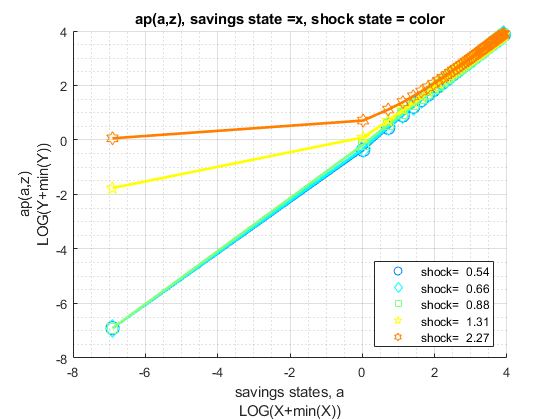
\includegraphics[width=5.20833in,height=\textheight]{img/fx_vfi_az_bisec_loop_images/figure_1.png}

Run the function and show summaries for savings and fraction of coh
saved:

\begin{verbatim}
mp_params('it_a_n') = 100;
mp_params('it_z_n') = 9;
mp_support('ls_ffcmd') = {'ap', 'savefraccoh'};
mp_support('ls_ffsna') = {};
mp_support('ls_ffgrh') = {};
mp_support('bl_vfi_store_all') = true; % store c(a,z), y(a,z)
ff_vfi_az_bisec_loop(mp_params, mp_support);

Elapsed time is 35.765637 seconds.
----------------------------------------
xxxxxxxxxxxxxxxxxxxxxxxxxxxxxxxxxxxxxxxx
CONTAINER NAME: mp_ffcmd ND Array (Matrix etc)
xxxxxxxxxxxxxxxxxxxxxxxxxxxxxxxxxxxxxxxx
                   i    idx    ndim    numel    rowN    colN     sum       mean       std      coefvari    min      max  
                   _    ___    ____    _____    ____    ____    ______    _______    ______    ________    ___    _______

    ap             1     1      2       900     100      9       21835     24.261    14.095    0.58096      0       51.61
    savefraccoh    2     2      2       900     100      9      754.27    0.83808    0.1259    0.15023      0     0.91596

xxx TABLE:ap xxxxxxxxxxxxxxxxxx
              c1         c2         c3         c4         c5          c6         c7         c8        c9  
            _______    _______    _______    _______    _______    ________    _______    ______    ______

    r1            0          0          0          0          0    0.082559    0.50504    1.2988    3.1416
    r2      0.26067    0.25936    0.26888    0.30308    0.39296     0.52492    0.96211    1.7672    3.6183
    r3      0.65383    0.65589    0.67297    0.71974    0.82473      1.0101     1.4185    2.2377    4.0955
    r4       1.0734     1.0789     1.1015     1.1556     1.2679      1.4909     1.8821    2.7095    4.5736
    r5       1.5151     1.5159     1.5427     1.6019       1.72      1.9489      2.349    3.1825    5.0521
    r96      45.547      45.58     45.636      45.73     45.888      46.134     46.603     47.52     49.54
    r97      46.036     46.069     46.126      46.22     46.377      46.622     47.092    48.009    50.057
    r98      46.525     46.559     46.615      46.71     46.867      47.112     47.583    48.501    50.575
    r99      47.014     47.049     47.104     47.198     47.357      47.601     48.072    48.992    51.092
    r100     47.503     47.537     47.593     47.687     47.845      48.091     48.561    49.495     51.61

xxx TABLE:savefraccoh xxxxxxxxxxxxxxxxxx
              c1         c2         c3         c4         c5          c6         c7         c8         c9   
            _______    _______    _______    _______    _______    ________    _______    _______    _______

    r1            0          0          0          0          0    0.056268    0.24587    0.41301    0.58272
    r2      0.23098      0.217    0.20843    0.21203    0.23925     0.26445     0.3741    0.48253    0.61235
    r3      0.39717    0.38292    0.37227    0.36965    0.38179     0.40361    0.45915    0.53532    0.63728
    r4      0.49605    0.48369    0.47368    0.46883    0.47347     0.49364    0.52177    0.57677    0.65861
    r5      0.56502    0.55159    0.54262    0.53709    0.53825     0.55086    0.56947    0.61021    0.67704
    r96     0.91477    0.91422    0.91361    0.91294    0.91221      0.9109    0.90961    0.90818    0.90781
    r97     0.91508    0.91453    0.91395    0.91328    0.91254     0.91123    0.90998    0.90855    0.90867
    r98     0.91538    0.91486    0.91425    0.91361    0.91288     0.91157    0.91035    0.90894    0.90952
    r99     0.91569    0.91517    0.91456    0.91392    0.91322      0.9119    0.91068    0.90934    0.91035
    r100    0.91596    0.91544    0.91486    0.91422    0.91352     0.91224    0.91102    0.90992    0.91117
\end{verbatim}

\hypertarget{test-ff_vfi_az_bisec_loop-change-interest-rate-and-discount}{%
\subsection{Test FF\_VFI\_AZ\_BISEC\_LOOP Change Interest Rate and Discount}\label{test-ff_vfi_az_bisec_loop-change-interest-rate-and-discount}}

Show only save fraction of cash on hand:

\begin{verbatim}
mp_support = containers.Map('KeyType','char', 'ValueType','any');
mp_support('bl_print_params') = false;
mp_support('bl_print_iterinfo') = false;
mp_support('ls_ffcmd') = {'savefraccoh'};
mp_support('ls_ffsna') = {};
mp_support('ls_ffgrh') = {};
mp_params = containers.Map('KeyType','char', 'ValueType','any');
mp_params('it_a_n') = 50;
mp_params('it_z_n') = 5;
mp_params('fl_a_max') = 50;
mp_params('st_grid_type') = 'grid_powerspace';
\end{verbatim}

Solve the model with several different interest rates and discount
factor:

\begin{verbatim}
% Lower Savings Incentives
mp_params('fl_beta') = 0.80;
mp_params('fl_r') = 0.01;
ff_vfi_az_bisec_loop(mp_params, mp_support);

Elapsed time is 2.672239 seconds.
----------------------------------------
xxxxxxxxxxxxxxxxxxxxxxxxxxxxxxxxxxxxxxxx
CONTAINER NAME: mp_ffcmd ND Array (Matrix etc)
xxxxxxxxxxxxxxxxxxxxxxxxxxxxxxxxxxxxxxxx
                   i    idx    ndim    numel    rowN    colN     sum       mean        std      coefvari    min      max  
                   _    ___    ____    _____    ____    ____    ______    _______    _______    ________    ___    _______

    savefraccoh    1     1      2       250      50      5      119.77    0.47907    0.28808    0.60133      0     0.80699

xxx TABLE:savefraccoh xxxxxxxxxxxxxxxxxx
             c1         c2         c3         c4         c5   
           _______    _______    _______    _______    _______

    r1           0          0          0          0    0.10641
    r2           0          0          0          0    0.10641
    r3           0          0          0          0    0.10629
    r4           0          0          0          0    0.10601
    r5           0          0          0          0    0.10793
    r46    0.79096    0.78788    0.78242    0.77293    0.76768
    r47    0.79554    0.79261    0.78749    0.77754    0.77168
    r48    0.79991    0.79716    0.79228    0.78291     0.7754
    r49    0.80406    0.80146    0.79688      0.788    0.77891
    r50    0.80699    0.80396     0.8003    0.79283    0.78218

% Higher Savings Incentives
mp_params('fl_beta') = 0.95;
mp_params('fl_r') = 0.04;
ff_vfi_az_bisec_loop(mp_params, mp_support);

Elapsed time is 11.445094 seconds.
----------------------------------------
xxxxxxxxxxxxxxxxxxxxxxxxxxxxxxxxxxxxxxxx
CONTAINER NAME: mp_ffcmd ND Array (Matrix etc)
xxxxxxxxxxxxxxxxxxxxxxxxxxxxxxxxxxxxxxxx
                   i    idx    ndim    numel    rowN    colN     sum       mean        std      coefvari    min      max  
                   _    ___    ____    _____    ____    ____    ______    _______    _______    ________    ___    _______

    savefraccoh    1     1      2       250      50      5      162.74    0.65097    0.29744    0.45693      0     0.92924

xxx TABLE:savefraccoh xxxxxxxxxxxxxxxxxx
             c1         c2          c3         c4         c5   
           _______    _______    ________    _______    _______

    r1           0          0    0.029138    0.21236    0.45384
    r2           0          0    0.029535    0.21258     0.4539
    r3           0          0     0.03219    0.21401    0.45448
    r4           0          0    0.039301    0.21795    0.45607
    r5           0          0    0.045923    0.22542    0.45909
    r46     0.9221    0.92124     0.92029    0.91929    0.91587
    r47    0.92408    0.92329     0.92237    0.92142    0.91816
    r48    0.92591    0.92518     0.92432    0.92344    0.92057
    r49    0.92762    0.92692     0.92612    0.92536    0.92347
    r50    0.92924     0.9286     0.92792    0.92737    0.92783
\end{verbatim}

\hypertarget{test-ff_vfi_az_bisec_loop-changing-risk-aversion}{%
\subsection{Test FF\_VFI\_AZ\_BISEC\_LOOP Changing Risk Aversion}\label{test-ff_vfi_az_bisec_loop-changing-risk-aversion}}

Here, again, show fraction of coh saved in summary tabular form, but
also show it graphically.

\begin{verbatim}
mp_support = containers.Map('KeyType','char', 'ValueType','any');
mp_support('bl_print_params') = false;
mp_support('bl_print_iterinfo') = false;
mp_support('ls_ffcmd') = {'savefraccoh'};
mp_support('ls_ffsna') = {};
mp_support('ls_ffgrh') = {'savefraccoh'};
mp_params = containers.Map('KeyType','char', 'ValueType','any');
mp_params('it_a_n') = 100;
mp_params('it_z_n') = 5;
mp_params('fl_a_max') = 50;
mp_params('st_grid_type') = 'grid_powerspace';
\end{verbatim}

Solve the model with different risk aversion levels, higher preferences
for risk:

\begin{verbatim}
% Lower Risk Aversion
mp_params('fl_crra') = 0.5;
ff_vfi_az_bisec_loop(mp_params, mp_support);

Elapsed time is 20.016228 seconds.
----------------------------------------
xxxxxxxxxxxxxxxxxxxxxxxxxxxxxxxxxxxxxxxx
CONTAINER NAME: mp_ffcmd ND Array (Matrix etc)
xxxxxxxxxxxxxxxxxxxxxxxxxxxxxxxxxxxxxxxx
                   i    idx    ndim    numel    rowN    colN     sum       mean        std      coefvari    min      max  
                   _    ___    ____    _____    ____    ____    ______    _______    _______    ________    ___    _______

    savefraccoh    1     1      2       500     100      5      270.24    0.54048    0.30018     0.5554      0     0.85804

xxx TABLE:savefraccoh xxxxxxxxxxxxxxxxxx
              c1         c2         c3          c4         c5   
            _______    _______    _______    ________    _______

    r1            0          0          0    0.016108    0.19552
    r2            0          0          0    0.016138    0.19555
    r3            0          0          0    0.016352    0.19564
    r4            0          0          0    0.016962    0.19591
    r5            0          0          0    0.018091    0.19646
    r96     0.85334    0.85127    0.84879     0.84602    0.84037
    r97     0.85456    0.85255    0.85017     0.84748     0.8419
    r98     0.85578    0.85383    0.85151     0.84889    0.84339
    r99     0.85694    0.85502    0.85279     0.85023    0.84483
    r100    0.85804    0.85621    0.85404     0.85154    0.84623
\end{verbatim}

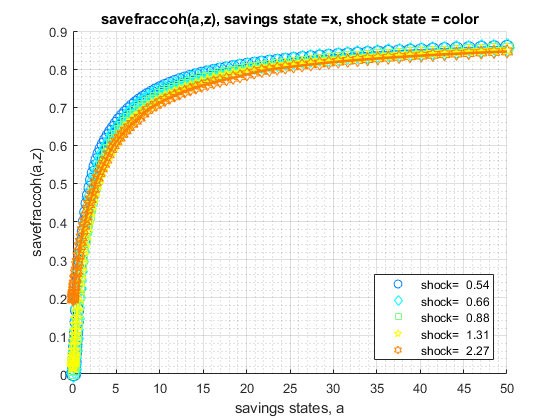
\includegraphics[width=5.20833in,height=\textheight]{img/fx_vfi_az_bisec_loop_images/figure_2.png}

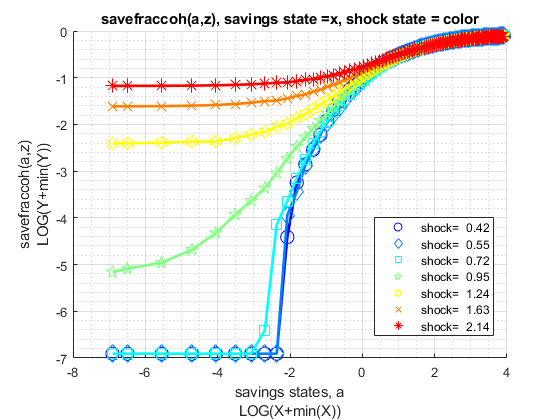
\includegraphics[width=5.20833in,height=\textheight]{img/fx_vfi_az_bisec_loop_images/figure_3.png}

When risk aversion increases, at every state-space point, the household
wants to save more.

\begin{verbatim}
% Higher Risk Aversion
mp_params('fl_crra') = 5;
ff_vfi_az_bisec_loop(mp_params, mp_support);

Elapsed time is 19.070686 seconds.
----------------------------------------
xxxxxxxxxxxxxxxxxxxxxxxxxxxxxxxxxxxxxxxx
CONTAINER NAME: mp_ffcmd ND Array (Matrix etc)
xxxxxxxxxxxxxxxxxxxxxxxxxxxxxxxxxxxxxxxx
                   i    idx    ndim    numel    rowN    colN     sum       mean        std      coefvari    min      max  
                   _    ___    ____    _____    ____    ____    ______    _______    _______    ________    ___    _______

    savefraccoh    1     1      2       500     100      5      337.39    0.67477    0.28798    0.42678      0     0.94089

xxx TABLE:savefraccoh xxxxxxxxxxxxxxxxxx
              c1         c2          c3         c4         c5   
            _______    _______    ________    _______    _______

    r1            0          0    0.082635     0.2781     0.5078
    r2            0          0    0.082665    0.27813     0.5078
    r3            0          0     0.08297    0.27828    0.50786
    r4            0          0    0.083794    0.27871    0.50801
    r5            0          0    0.085381    0.27956    0.50835
    r96     0.93751    0.93699     0.93641    0.93586    0.93482
    r97     0.93839     0.9379     0.93732     0.9368    0.93586
    r98     0.93925    0.93876     0.93824    0.93775    0.93702
    r99      0.9401    0.93961     0.93909    0.93867    0.93839
    r100    0.94089    0.94044     0.93998    0.93961    0.94013
\end{verbatim}

\includegraphics[width=5.20833in,height=\textheight]{img/fx_vfi_az_bisec_loop_images/figure_4.png}

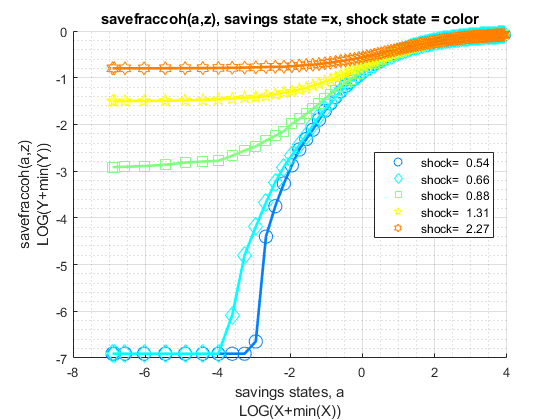
\includegraphics[width=5.20833in,height=\textheight]{img/fx_vfi_az_bisec_loop_images/figure_5.png}

\hypertarget{test-ff_vfi_az_bisec_loop-with-higher-uncertainty}{%
\subsection{Test FF\_VFI\_AZ\_BISEC\_LOOP with Higher Uncertainty}\label{test-ff_vfi_az_bisec_loop-with-higher-uncertainty}}

Increase the standard deviation of the Shock.

\begin{verbatim}
mp_support = containers.Map('KeyType','char', 'ValueType','any');
mp_support('bl_print_params') = false;
mp_support('bl_print_iterinfo') = false;
mp_support('ls_ffcmd') = {'savefraccoh'};
mp_support('ls_ffsna') = {};
mp_support('ls_ffgrh') = {};
mp_params = containers.Map('KeyType','char', 'ValueType','any');
mp_params('it_a_n') = 100;
mp_params('it_z_n') = 5;
mp_params('fl_a_max') = 50;
mp_params('st_grid_type') = 'grid_powerspace';
\end{verbatim}

Lower standard deviation of shock:

\begin{verbatim}
% Lower Risk Aversion
mp_params('fl_shk_std') = 0.10;
ff_vfi_az_bisec_loop(mp_params, mp_support);

Elapsed time is 19.744605 seconds.
----------------------------------------
xxxxxxxxxxxxxxxxxxxxxxxxxxxxxxxxxxxxxxxx
CONTAINER NAME: mp_ffcmd ND Array (Matrix etc)
xxxxxxxxxxxxxxxxxxxxxxxxxxxxxxxxxxxxxxxx
                   i    idx    ndim    numel    rowN    colN     sum       mean        std      coefvari    min     max  
                   _    ___    ____    _____    ____    ____    ______    _______    _______    ________    ___    ______

    savefraccoh    1     1      2       500     100      5      295.24    0.59048    0.32213    0.54554      0     0.9127

xxx TABLE:savefraccoh xxxxxxxxxxxxxxxxxx
              c1         c2         c3          c4         c5   
            _______    _______    _______    ________    _______

    r1            0          0          0    0.030451    0.12142
    r2            0          0          0    0.030481    0.12145
    r3            0          0          0    0.030725    0.12164
    r4            0          0          0    0.031366    0.12209
    r5            0          0          0    0.032648    0.12304
    r96     0.90824    0.90775    0.90726     0.90675    0.90629
    r97     0.90943    0.90894    0.90845     0.90797    0.90751
    r98     0.91056     0.9101    0.90961     0.90916     0.9087
    r99     0.91166     0.9112    0.91074     0.91029    0.90983
    r100     0.9127    0.91227    0.91184     0.91138    0.91096
\end{verbatim}

Higher shock standard deviation: low shock high asset save more, high
shock more asset save less, high shock low asset save more:

\begin{verbatim}
% Higher Risk Aversion
mp_params('fl_shk_std') = 0.40;
ff_vfi_az_bisec_loop(mp_params, mp_support);

Elapsed time is 17.556461 seconds.
----------------------------------------
xxxxxxxxxxxxxxxxxxxxxxxxxxxxxxxxxxxxxxxx
CONTAINER NAME: mp_ffcmd ND Array (Matrix etc)
xxxxxxxxxxxxxxxxxxxxxxxxxxxxxxxxxxxxxxxx
                   i    idx    ndim    numel    rowN    colN     sum       mean        std      coefvari    min      max  
                   _    ___    ____    _____    ____    ____    ______    _______    _______    ________    ___    _______

    savefraccoh    1     1      2       500     100      5      354.06    0.70811    0.27055    0.38207      0     0.92811

xxx TABLE:savefraccoh xxxxxxxxxxxxxxxxxx
              c1         c2          c3         c4         c5   
            _______    _______    ________    _______    _______

    r1            0          0    0.030725    0.36968    0.77064
    r2            0          0    0.030725    0.36968    0.77064
    r3            0          0    0.030695    0.36959    0.77064
    r4            0          0    0.030634    0.36934    0.77061
    r5            0          0    0.030542    0.36885    0.77043
    r96     0.92429    0.92289     0.92091    0.91688    0.92026
    r97     0.92496    0.92362     0.92173    0.91795    0.92231
    r98     0.92564    0.92432     0.92252    0.91898    0.92429
    r99     0.92628    0.92503     0.92332    0.91999    0.92625
    r100    0.92689     0.9257     0.92408    0.92103    0.92811
\end{verbatim}

\hypertarget{ff_vfi_az_bisec_vec-dynamic-savings-problem-vectorized-continuous-exact}{%
\section{FF\_VFI\_AZ\_BISEC\_VEC Dynamic Savings Problem Vectorized Continuous Exact}\label{ff_vfi_az_bisec_vec-dynamic-savings-problem-vectorized-continuous-exact}}

\begin{quote}
Go back to \href{http://fanwangecon.github.io/}{fan}'s \href{https://fanwangecon.github.io/MEconTools/}{MEconTools} Toolbox (\href{https://fanwangecon.github.io/MEconTools/bookdown}{bookdown}), \href{https://fanwangecon.github.io/M4Econ/}{Matlab Code Examples} Repository (\href{https://fanwangecon.github.io/M4Econ/bookdown}{bookdown}), or \href{https://fanwangecon.github.io/Math4Econ/}{Math for Econ with Matlab} Repository (\href{https://fanwangecon.github.io/Math4Econ/bookdown}{bookdown}).
\end{quote}

This is the example vignette for function:
\href{https://github.com/FanWangEcon/MEconTools/blob/master/MEconTools/vfi/ff_vfi_az_bisec_vec.m}{\textbf{ff\_vfi\_az\_bisec\_vec}}
from the \href{https://fanwangecon.github.io/MEconTools/}{\textbf{MEconTools
Package}}\textbf{.} This function
solves the dynamic programming problem for a (a,z) model. Households can
save a, and face AR(1) shock z. The problem is solved over the infinite
horizon. This is a vectorized code, it is much faster for larger
state-space problems then looped code.

The code uses continuous choices, solved with bi(multi)section. The
state-space is on a grid, but choice grids are in terms of percentage of
resources available, which is individual specific, to save and solved
exactly up to ((1/(2)\^{}16)*100=0.001525878) percentage of cash on hand.
THe
\href{https://github.com/FanWangEcon/MEconTools/blob/master/MEconTools/vfi/ff_vfi_az_vec.m}{\textbf{ff\_vfi\_az\_vec}}
from the \href{https://fanwangecon.github.io/MEconTools/}{\textbf{MEconTools
Package}} solves the same
problem using vectorized common grid code where the choice set and state
space share the same grid.

This is the vectorized code, its speed is much faster than the looped
code. The function is designed to have small memory footprint and
requires low computing resources, yet is fast.

\textbf{Links to Four Code:}

Four Core Savings/Borrowing Dynamic Programming Solution Functions that
are functions in the \href{https://fanwangecon.github.io/MEconTools/}{\textbf{MEconTools
Package}}\textbf{.} :

\begin{itemize}
\item
  Common Choice and States Grid :
  \href{https://github.com/FanWangEcon/MEconTools/blob/master/MEconTools/vfi/ff_vfi_az_loop.m}{\textbf{ff\_vfi\_az\_loop}},
  slow should use for testing new models
\item
  Common Choice and States Grid :
  \href{https://github.com/FanWangEcon/MEconTools/blob/master/MEconTools/vfi/ff_vfi_az_vec.m}{\textbf{ff\_vfi\_az\_vec}},
  fast good for many purposes
\item
  States Grid + Continuous Exact Savings as Share of Cash-on-Hand :\href{https://github.com/FanWangEcon/MEconTools/blob/master/MEconTools/vfi/ff_vfi_az_bisec_loop.m}{\textbf{ff\_vfi\_az\_bisec\_loop}},
  high precision even with small grid
\item
  States Grid + Continuous Exact Savings as Share of Cash-on-Hand :
  \href{https://github.com/FanWangEcon/MEconTools/blob/master/MEconTools/vfi/ff_vfi_az_bisec_vec.m}{\textbf{ff\_vfi\_az\_bisec\_vec}},
  precision and speed
\end{itemize}

\hypertarget{test-ff_vfi_az_bisec_vec-defaults}{%
\subsection{Test FF\_VFI\_AZ\_BISEC\_VEC Defaults}\label{test-ff_vfi_az_bisec_vec-defaults}}

Call the function with defaults. By default, shows the asset policy
function summary. Model parameters can be changed by the mp\_params.

\begin{verbatim}
%mp_params
mp_params = containers.Map('KeyType','char', 'ValueType','any');
mp_params('fl_crra') = 1.5;
mp_params('fl_beta') = 0.94;
% call function
ff_vfi_az_bisec_vec(mp_params);

Elapsed time is 0.668798 seconds.
----------------------------------------
xxxxxxxxxxxxxxxxxxxxxxxxxxxxxxxxxxxxxxxx
CONTAINER NAME: mp_ffcmd ND Array (Matrix etc)
xxxxxxxxxxxxxxxxxxxxxxxxxxxxxxxxxxxxxxxx
          i    idx    ndim    numel    rowN    colN     sum      mean      std      coefvari    min     max  
          _    ___    ____    _____    ____    ____    _____    ______    ______    ________    ___    ______

    ap    1     1      2       700     100      7      16866    24.094    14.071    0.58399      0     50.252

xxx TABLE:ap xxxxxxxxxxxxxxxxxx
              c1         c2         c3         c4         c5         c6         c7  
            _______    _______    _______    _______    _______    _______    ______

    r1            0          0          0          0    0.13188    0.66203    1.9859
    r2      0.25914    0.26426    0.29511    0.39221    0.57697     1.1208    2.4569
    r3      0.65371    0.66543    0.70966    0.82502      1.029      1.582    2.9298
    r4       1.0748     1.0921     1.1447     1.2698     1.5151     2.0481    3.4046
    r5       1.5152     1.5319     1.5903      1.721     2.0011     2.5252    3.8802
    r96      45.561     45.615     45.712     45.887     46.192     46.835    48.252
    r97      46.049     46.104     46.201     46.377     46.681     47.325    48.743
    r98       46.54     46.593      46.69     46.866     47.171     47.815    49.235
    r99      47.029     47.082     47.179     47.356     47.661     48.304    49.734
    r100     47.518     47.572      47.67     47.845      48.15     48.793    50.252
\end{verbatim}

\hypertarget{test-ff_vfi_az_bisec_vec-speed-tests-1}{%
\subsection{Test FF\_VFI\_AZ\_BISEC\_VEC Speed Tests}\label{test-ff_vfi_az_bisec_vec-speed-tests-1}}

Call the function with defaults. By default, shows the asset policy
function summary. Model parameters can be changed by the mp\_params.

\begin{verbatim}
mp_support = containers.Map('KeyType','char', 'ValueType','any');
mp_support('bl_timer') = true;
mp_support('ls_ffcmd') = {};
\end{verbatim}

A grid 50, shock grid 5:

\begin{verbatim}
mp_params = containers.Map('KeyType','char', 'ValueType','any');
mp_params('it_a_n') = 50;
mp_params('it_z_n') = 5;
ff_vfi_az_bisec_vec(mp_params, mp_support);

Elapsed time is 0.336083 seconds.
\end{verbatim}

A grid 750, shock grid 15:

\begin{verbatim}
mp_params = containers.Map('KeyType','char', 'ValueType','any');
mp_params('it_a_n') = 750;
mp_params('it_z_n') = 15;
ff_vfi_az_bisec_vec(mp_params, mp_support);

Elapsed time is 23.612756 seconds.
\end{verbatim}

A grid 600, shock grid 45:

\begin{verbatim}
mp_params = containers.Map('KeyType','char', 'ValueType','any');
mp_params('it_a_n') = 600;
mp_params('it_z_n') = 45;
ff_vfi_az_bisec_vec(mp_params, mp_support);

Elapsed time is 46.281741 seconds.
\end{verbatim}

\hypertarget{test-ff_vfi_az_bisec_vec-control-outputs}{%
\subsection{Test FF\_VFI\_AZ\_BISEC\_VEC Control Outputs}\label{test-ff_vfi_az_bisec_vec-control-outputs}}

Run the function first without any outputs;

\begin{verbatim}
mp_params = containers.Map('KeyType','char', 'ValueType','any');
mp_params('it_a_n') = 50;
mp_params('it_z_n') = 5;
mp_support = containers.Map('KeyType','char', 'ValueType','any');
mp_support('bl_timer') = false;
mp_support('bl_print_params') = false;
mp_support('bl_print_iterinfo') = false;
\end{verbatim}

Run the function and show policy function for savings choice. For
ls\_ffcmd, ls\_ffsna, ls\_ffgrh, can include these: `v', `ap', `c', `y',
`coh', `savefraccoh'. These are value, aprime savings choice,
consumption, income, cash on hand, and savings fraction as cash-on-hand.

\begin{verbatim}
mp_support = containers.Map('KeyType','char', 'ValueType','any');
mp_support('bl_print_params') = false;
mp_support('bl_print_iterinfo') = false;
% ls_ffcmd: summary print which outcomes
mp_support('ls_ffcmd') = {};
% ls_ffsna: detail print which outcomes
mp_support('ls_ffsna') = {'savefraccoh'};
% ls_ffgrh: graphical print which outcomes
mp_support('ls_ffgrh') = {'savefraccoh'};
ff_vfi_az_bisec_vec(mp_params, mp_support);

Elapsed time is 0.470134 seconds.
xxx  ff_vfi_az_vec, outcome=savefraccoh  xxxxxxxxxxxxxxxxxxxxxxxxxxx
    group      a       mean_z_0_54195    mean_z_0_66401    mean_z_0_88162    mean_z_1_3095    mean_z_2_2745
    _____    ______    ______________    ______________    ______________    _____________    _____________

      1           0             0                 0                 0           0.10165          0.36531   
      2      1.0204       0.39833           0.38191           0.38826           0.40373          0.51573   
      3      2.0408       0.56236           0.54875           0.54619           0.54161          0.61104   
      4      3.0612       0.64616           0.63545            0.6306           0.63591          0.66349   
      5      4.0816       0.69783            0.6891            0.6837            0.6873          0.70155   
      6       5.102       0.73323            0.7259           0.72068           0.72184           0.7302   
      7      6.1224       0.75917           0.75291           0.74803           0.74784          0.75257   
      8      7.1429       0.77909           0.77363           0.76911           0.76817          0.77058   
      9      8.1633       0.79493           0.79011           0.78593           0.78452          0.78541   
     10      9.1837       0.80787           0.80354           0.79969           0.79801          0.79783   
     11      10.204       0.82343           0.81474           0.81114            0.8093          0.80839   
     12      11.224       0.83412           0.82591           0.82084           0.81895          0.81748   
     13      12.245       0.84116           0.83759           0.82917           0.82725          0.82542   
     14      13.265       0.84733           0.84434           0.83637           0.83448          0.83241   
     15      14.286       0.85282           0.84998           0.84272           0.84083          0.83857   
     16      15.306        0.8577           0.85508           0.84947           0.84647          0.84406   
     17      16.327       0.86213           0.85966           0.85685           0.85151          0.84901   
     18      17.347       0.86613           0.86378           0.86143             0.856          0.85349   
     19      18.367       0.86976            0.8675           0.86521           0.86008          0.85755   
     20      19.388       0.87305           0.87092           0.86869           0.86384          0.86128   
     21      20.408       0.87608           0.87403            0.8719           0.86726          0.86472   
     22      21.429       0.87885            0.8769           0.87486            0.8704           0.8679   
     23      22.449       0.88145           0.87955            0.8776           0.87333          0.87083   
     24      23.469       0.88383           0.88203           0.88013           0.87601          0.87354   
     25       24.49       0.88602           0.88432           0.88248           0.87852          0.87608   
     26       25.51        0.8881           0.88645           0.88468           0.88087          0.87843   
     27      26.531       0.89002           0.88844           0.88673           0.88361          0.88126   
     28      27.551       0.89185           0.89033           0.88865           0.88685          0.88444   
     29      28.571       0.89353           0.89207           0.89045           0.88895          0.88636   
     30      29.592       0.89515           0.89371           0.89216           0.89063          0.88813   
     31      30.612       0.89664           0.89527           0.89375           0.89225          0.88978   
     32      31.633       0.89808           0.89674           0.89524           0.89378          0.89136   
     33      32.653       0.89942           0.89811           0.89667           0.89521          0.89286   
     34      33.673       0.90067           0.89942           0.89802           0.89658          0.89429   
     35      34.694       0.90189           0.90067            0.8993            0.8979          0.89564   
     36      35.714       0.90305           0.90186           0.90052           0.89915          0.89692   
     37      36.735       0.90473           0.90299           0.90168           0.90034          0.89814   
     38      37.755       0.90662           0.90406           0.90278           0.90147          0.89933   
     39      38.776       0.90763           0.90507           0.90382           0.90256          0.90043   
     40      39.796       0.90852           0.90668           0.90482           0.90357           0.9015   
     41      40.816       0.90937           0.90833            0.9058           0.90458          0.90253   
     42      41.837       0.91019           0.90919           0.90671           0.90552          0.90351   
     43      42.857       0.91099           0.91001            0.9076           0.90641          0.90446   
     44      43.878       0.91172           0.91077           0.90842           0.90729          0.90534   
     45      44.898       0.91245           0.91154           0.90925           0.90812           0.9062   
     46      45.918       0.91315           0.91224           0.91041           0.90891          0.90702   
     47      46.939       0.91383           0.91294           0.91181           0.90971          0.90784   
     48      47.959        0.9145           0.91361           0.91264           0.91044          0.90861   
     49       48.98       0.91511           0.91425           0.91328           0.91114          0.90934   
     50          50       0.91572           0.91486           0.91392           0.91181          0.91004   
\end{verbatim}

\includegraphics[width=5.20833in,height=\textheight]{img/fx_vfi_az_bisec_vec_images/figure_0.png}

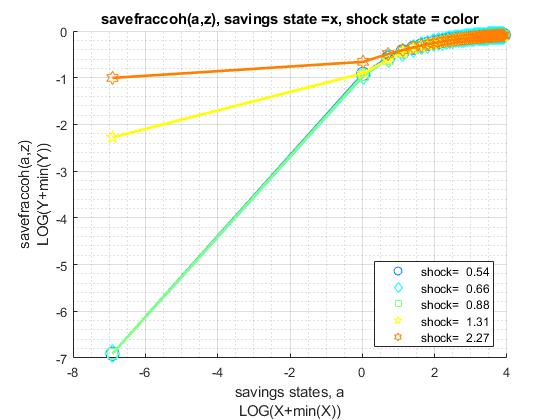
\includegraphics[width=5.20833in,height=\textheight]{img/fx_vfi_az_bisec_vec_images/figure_1.png}

Run the function and show summaries for savings and fraction of coh
saved:

\begin{verbatim}
mp_params('it_a_n') = 100;
mp_params('it_z_n') = 9;
mp_support('ls_ffcmd') = {'ap', 'savefraccoh'};
mp_support('ls_ffsna') = {};
mp_support('ls_ffgrh') = {};
mp_support('bl_vfi_store_all') = true; % store c(a,z), y(a,z)
ff_vfi_az_bisec_vec(mp_params, mp_support);

Elapsed time is 0.716025 seconds.
----------------------------------------
xxxxxxxxxxxxxxxxxxxxxxxxxxxxxxxxxxxxxxxx
CONTAINER NAME: mp_ffcmd ND Array (Matrix etc)
xxxxxxxxxxxxxxxxxxxxxxxxxxxxxxxxxxxxxxxx
                   i    idx    ndim    numel    rowN    colN     sum       mean       std      coefvari    min      max  
                   _    ___    ____    _____    ____    ____    ______    _______    ______    ________    ___    _______

    ap             1     1      2       900     100      9       21835     24.261    14.095    0.58096      0       51.61
    savefraccoh    2     2      2       900     100      9      754.27    0.83808    0.1259    0.15023      0     0.91596

xxx TABLE:ap xxxxxxxxxxxxxxxxxx
              c1         c2         c3         c4         c5          c6         c7         c8        c9  
            _______    _______    _______    _______    _______    ________    _______    ______    ______

    r1            0          0          0          0          0    0.082559    0.50504    1.2988    3.1416
    r2      0.26067    0.25936    0.26888    0.30308    0.39296     0.52492    0.96211    1.7672    3.6183
    r3      0.65383    0.65589    0.67297    0.71974    0.82473      1.0101     1.4185    2.2377    4.0955
    r4       1.0734     1.0789     1.1015     1.1556     1.2679      1.4909     1.8821    2.7095    4.5736
    r5       1.5151     1.5159     1.5427     1.6019       1.72      1.9489      2.349    3.1825    5.0521
    r96      45.547      45.58     45.636      45.73     45.888      46.134     46.603     47.52     49.54
    r97      46.036     46.069     46.126      46.22     46.377      46.622     47.092    48.009    50.057
    r98      46.525     46.559     46.615      46.71     46.867      47.112     47.583    48.501    50.575
    r99      47.014     47.049     47.104     47.198     47.357      47.601     48.072    48.992    51.092
    r100     47.503     47.537     47.593     47.687     47.845      48.091     48.561    49.495     51.61

xxx TABLE:savefraccoh xxxxxxxxxxxxxxxxxx
              c1         c2         c3         c4         c5          c6         c7         c8         c9   
            _______    _______    _______    _______    _______    ________    _______    _______    _______

    r1            0          0          0          0          0    0.056268    0.24587    0.41301    0.58272
    r2      0.23098      0.217    0.20843    0.21203    0.23925     0.26445     0.3741    0.48253    0.61235
    r3      0.39717    0.38292    0.37227    0.36965    0.38179     0.40361    0.45915    0.53532    0.63728
    r4      0.49605    0.48369    0.47368    0.46883    0.47347     0.49364    0.52177    0.57677    0.65861
    r5      0.56502    0.55159    0.54262    0.53709    0.53825     0.55086    0.56947    0.61021    0.67704
    r96     0.91477    0.91422    0.91361    0.91294    0.91221      0.9109    0.90961    0.90818    0.90781
    r97     0.91508    0.91453    0.91395    0.91328    0.91254     0.91123    0.90998    0.90855    0.90867
    r98     0.91538    0.91486    0.91425    0.91361    0.91288     0.91157    0.91035    0.90894    0.90952
    r99     0.91569    0.91517    0.91456    0.91392    0.91322      0.9119    0.91068    0.90934    0.91035
    r100    0.91596    0.91544    0.91486    0.91422    0.91352     0.91224    0.91102    0.90992    0.91117
\end{verbatim}

\hypertarget{test-ff_vfi_az_bisec_vec-change-interest-rate-and-discount}{%
\subsection{Test FF\_VFI\_AZ\_BISEC\_VEC Change Interest Rate and Discount}\label{test-ff_vfi_az_bisec_vec-change-interest-rate-and-discount}}

Show only save fraction of cash on hand:

\begin{verbatim}
mp_support = containers.Map('KeyType','char', 'ValueType','any');
mp_support('bl_print_params') = false;
mp_support('bl_print_iterinfo') = false;
mp_support('ls_ffcmd') = {'savefraccoh'};
mp_support('ls_ffsna') = {};
mp_support('ls_ffgrh') = {};
mp_params = containers.Map('KeyType','char', 'ValueType','any');
mp_params('it_a_n') = 750;
mp_params('it_z_n') = 9;
mp_params('fl_a_max') = 50;
mp_params('st_grid_type') = 'grid_powerspace';
\end{verbatim}

Solve the model with several different interest rates and discount
factor:

\begin{verbatim}
% Lower Savings Incentives
mp_params('fl_beta') = 0.80;
mp_params('fl_r') = 0.01;
ff_vfi_az_bisec_vec(mp_params, mp_support);

Elapsed time is 4.541023 seconds.
----------------------------------------
xxxxxxxxxxxxxxxxxxxxxxxxxxxxxxxxxxxxxxxx
CONTAINER NAME: mp_ffcmd ND Array (Matrix etc)
xxxxxxxxxxxxxxxxxxxxxxxxxxxxxxxxxxxxxxxx
                   i    idx    ndim    numel    rowN    colN     sum       mean        std      coefvari    min      max  
                   _    ___    ____    _____    ____    ____    ______    _______    _______    ________    ___    _______

    savefraccoh    1     1      2      6750     750      9      3318.4    0.49162    0.27766    0.56478      0     0.80534

xxx TABLE:savefraccoh xxxxxxxxxxxxxxxxxx
              c1         c2         c3         c4         c5         c6          c7         c8         c9   
            _______    _______    _______    _______    _______    _______    ________    _______    _______

    r1            0          0          0          0          0          0    0.023584     0.1329    0.29705
    r2            0          0          0          0          0          0    0.023584     0.1329    0.29705
    r3            0          0          0          0          0          0    0.023584     0.1329    0.29705
    r4            0          0          0          0          0          0    0.023584     0.1329    0.29705
    r5            0          0          0          0          0          0    0.023584     0.1329    0.29705
    r746    0.80439    0.80299    0.80094    0.79856    0.79588    0.79222     0.78825    0.78263    0.77647
    r747    0.80467    0.80314     0.8011    0.79875    0.79606     0.7924     0.78846    0.78285    0.77687
    r748    0.80491    0.80329    0.80125     0.7989    0.79621    0.79255     0.78864    0.78315    0.77732
    r749    0.80515    0.80341    0.80137    0.79905     0.7964    0.79273     0.78883    0.78352    0.77769
    r750    0.80534    0.80357    0.80152     0.7992    0.79655    0.79292     0.78904    0.78388     0.7779

% Higher Savings Incentives
mp_params('fl_beta') = 0.95;
mp_params('fl_r') = 0.04;
ff_vfi_az_bisec_vec(mp_params, mp_support);

Elapsed time is 17.994960 seconds.
----------------------------------------
xxxxxxxxxxxxxxxxxxxxxxxxxxxxxxxxxxxxxxxx
CONTAINER NAME: mp_ffcmd ND Array (Matrix etc)
xxxxxxxxxxxxxxxxxxxxxxxxxxxxxxxxxxxxxxxx
                   i    idx    ndim    numel    rowN    colN     sum       mean        std      coefvari    min     max  
                   _    ___    ____    _____    ____    ____    ______    _______    _______    ________    ___    ______

    savefraccoh    1     1      2      6750     750      9      4493.5    0.66571    0.28784    0.43238      0     0.9293

xxx TABLE:savefraccoh xxxxxxxxxxxxxxxxxx
              c1         c2         c3         c4          c5         c6         c7         c8         c9   
            _______    _______    _______    _______    ________    _______    _______    _______    _______

    r1            0          0          0          0    0.032007    0.15008    0.31087    0.48467    0.64488
    r2            0          0          0          0    0.032007    0.15008    0.31087    0.48467    0.64488
    r3            0          0          0          0    0.032007    0.15008    0.31087    0.48467    0.64488
    r4            0          0          0          0    0.032007    0.15008    0.31087    0.48467    0.64488
    r5            0          0          0          0    0.032007    0.15008    0.31087    0.48467    0.64488
    r746     0.9289     0.9285    0.92805    0.92734     0.92664    0.92594    0.92515    0.92545    0.92777
    r747    0.92902     0.9286    0.92814    0.92747     0.92673    0.92606     0.9253    0.92573    0.92802
    r748    0.92911    0.92869    0.92826    0.92756     0.92686    0.92618    0.92545      0.926    0.92829
    r749    0.92921    0.92881    0.92835    0.92768     0.92698    0.92631    0.92564    0.92631    0.92857
    r750     0.9293     0.9289    0.92844    0.92777     0.92707    0.92643    0.92591    0.92658    0.92881
\end{verbatim}

\hypertarget{test-ff_vfi_az_bisec_vec-changing-risk-aversion}{%
\subsection{Test FF\_VFI\_AZ\_BISEC\_VEC Changing Risk Aversion}\label{test-ff_vfi_az_bisec_vec-changing-risk-aversion}}

Here, again, show fraction of coh saved in summary tabular form, but
also show it graphically.

\begin{verbatim}
mp_support = containers.Map('KeyType','char', 'ValueType','any');
mp_support('bl_print_params') = false;
mp_support('bl_print_iterinfo') = false;
mp_support('ls_ffcmd') = {'savefraccoh'};
mp_support('ls_ffsna') = {};
mp_support('ls_ffgrh') = {'savefraccoh'};
mp_params = containers.Map('KeyType','char', 'ValueType','any');
mp_params('it_a_n') = 750;
mp_params('it_z_n') = 9;
mp_params('fl_a_max') = 50;
mp_params('st_grid_type') = 'grid_powerspace';
\end{verbatim}

Solve the model with different risk aversion levels, higher preferences
for risk:

\begin{verbatim}
% Lower Risk Aversion
mp_params('fl_crra') = 0.5;
ff_vfi_az_bisec_vec(mp_params, mp_support);

Elapsed time is 13.815578 seconds.
----------------------------------------
xxxxxxxxxxxxxxxxxxxxxxxxxxxxxxxxxxxxxxxx
CONTAINER NAME: mp_ffcmd ND Array (Matrix etc)
xxxxxxxxxxxxxxxxxxxxxxxxxxxxxxxxxxxxxxxx
                   i    idx    ndim    numel    rowN    colN     sum       mean        std      coefvari    min      max  
                   _    ___    ____    _____    ____    ____    ______    _______    _______    ________    ___    _______

    savefraccoh    1     1      2      6750     750      9      3735.7    0.55343    0.28972     0.5235      0     0.85999

xxx TABLE:savefraccoh xxxxxxxxxxxxxxxxxx
              c1         c2         c3         c4         c5         c6          c7         c8         c9   
            _______    _______    _______    _______    _______    _______    ________    _______    _______

    r1            0          0          0          0          0          0    0.074609    0.22661    0.41036
    r2            0          0          0          0          0          0    0.074609    0.22661    0.41036
    r3            0          0          0          0          0          0    0.074609    0.22661    0.41036
    r4            0          0          0          0          0          0    0.074609    0.22661    0.41036
    r5            0          0          0          0          0          0    0.074609    0.22664    0.41039
    r746    0.85941    0.85828    0.85703     0.8556    0.85398    0.85178     0.84907    0.84583    0.84211
    r747    0.85957    0.85844    0.85719    0.85575    0.85413    0.85194     0.84925    0.84602    0.84229
    r748    0.85969    0.85859    0.85734     0.8559    0.85429    0.85212     0.84943     0.8462    0.84248
    r749    0.85984    0.85871    0.85749    0.85606    0.85447    0.85227     0.84962    0.84638    0.84266
    r750    0.85999    0.85889    0.85761    0.85621    0.85462    0.85246     0.84977    0.84657    0.84284
\end{verbatim}

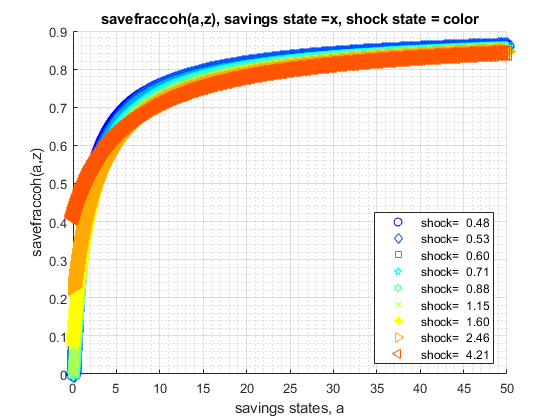
\includegraphics[width=5.20833in,height=\textheight]{img/fx_vfi_az_bisec_vec_images/figure_2.png}

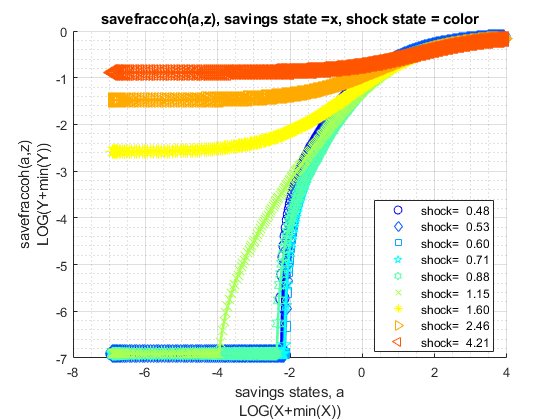
\includegraphics[width=5.20833in,height=\textheight]{img/fx_vfi_az_bisec_vec_images/figure_3.png}

When risk aversion increases, at every state-space point, the household
wants to save more.

\begin{verbatim}
% Higher Risk Aversion
mp_params('fl_crra') = 5;
ff_vfi_az_bisec_vec(mp_params, mp_support);

Elapsed time is 13.688997 seconds.
----------------------------------------
xxxxxxxxxxxxxxxxxxxxxxxxxxxxxxxxxxxxxxxx
CONTAINER NAME: mp_ffcmd ND Array (Matrix etc)
xxxxxxxxxxxxxxxxxxxxxxxxxxxxxxxxxxxxxxxx
                   i    idx    ndim    numel    rowN    colN    sum      mean       std      coefvari    min      max  
                   _    ___    ____    _____    ____    ____    ____    _______    ______    ________    ___    _______

    savefraccoh    1     1      2      6750     750      9      4640    0.68741    0.2821    0.41039      0     0.94169

xxx TABLE:savefraccoh xxxxxxxxxxxxxxxxxx
              c1         c2         c3          c4           c5         c6         c7         c8         c9   
            _______    _______    _______    _________    ________    _______    _______    _______    _______

    r1            0          0          0    0.0089972    0.085107    0.21343    0.37139    0.53578    0.68562
    r2            0          0          0    0.0089972    0.085107    0.21343    0.37139    0.53578    0.68562
    r3            0          0          0    0.0089972    0.085107    0.21343    0.37139    0.53578    0.68562
    r4            0          0          0    0.0089972    0.085107    0.21343    0.37139    0.53578    0.68562
    r5            0          0          0    0.0089972    0.085107    0.21343    0.37139    0.53578    0.68562
    r746    0.94105    0.94074    0.94041      0.93992     0.93943    0.93897    0.93848    0.93885    0.94083
    r747    0.94114    0.94083    0.94053      0.94004     0.93955    0.93909    0.93864    0.93909    0.94105
    r748    0.94126    0.94095    0.94062      0.94016     0.93964    0.93922    0.93879    0.93931    0.94126
    r749    0.94135    0.94105    0.94074      0.94025     0.93976    0.93934    0.93894    0.93955    0.94147
    r750    0.94144    0.94117    0.94083      0.94038     0.93989    0.93946    0.93915    0.93976    0.94169
\end{verbatim}

\includegraphics[width=5.20833in,height=\textheight]{img/fx_vfi_az_bisec_vec_images/figure_4.png}

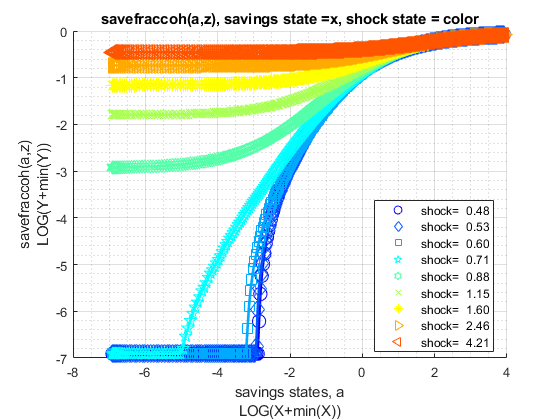
\includegraphics[width=5.20833in,height=\textheight]{img/fx_vfi_az_bisec_vec_images/figure_5.png}

\hypertarget{test-ff_vfi_az_bisec_vec-with-higher-uncertainty}{%
\subsection{Test FF\_VFI\_AZ\_BISEC\_VEC with Higher Uncertainty}\label{test-ff_vfi_az_bisec_vec-with-higher-uncertainty}}

Increase the standard deviation of the Shock.

\begin{verbatim}
mp_support = containers.Map('KeyType','char', 'ValueType','any');
mp_support('bl_print_params') = false;
mp_support('bl_print_iterinfo') = false;
mp_support('ls_ffcmd') = {'savefraccoh'};
mp_support('ls_ffsna') = {};
mp_support('ls_ffgrh') = {};
mp_params = containers.Map('KeyType','char', 'ValueType','any');
mp_params('it_a_n') = 750;
mp_params('it_z_n') = 9;
mp_params('fl_a_max') = 50;
mp_params('st_grid_type') = 'grid_powerspace';
\end{verbatim}

Lower standard deviation of shock:

\begin{verbatim}
% Lower Risk Aversion
mp_params('fl_shk_std') = 0.10;
ff_vfi_az_bisec_vec(mp_params, mp_support);

Elapsed time is 14.533433 seconds.
----------------------------------------
xxxxxxxxxxxxxxxxxxxxxxxxxxxxxxxxxxxxxxxx
CONTAINER NAME: mp_ffcmd ND Array (Matrix etc)
xxxxxxxxxxxxxxxxxxxxxxxxxxxxxxxxxxxxxxxx
                   i    idx    ndim    numel    rowN    colN     sum       mean       std      coefvari    min      max  
                   _    ___    ____    _____    ____    ____    ______    _______    ______    ________    ___    _______

    savefraccoh    1     1      2      6750     750      9      4025.4    0.59636    0.3153     0.5287      0     0.91331

xxx TABLE:savefraccoh xxxxxxxxxxxxxxxxxx
              c1         c2         c3         c4         c5          c6          c7         c8         c9   
            _______    _______    _______    _______    _______    ________    ________    _______    _______

    r1            0          0          0          0          0    0.012568    0.063073    0.13604    0.22228
    r2            0          0          0          0          0    0.012568    0.063073    0.13604    0.22228
    r3            0          0          0          0          0    0.012598    0.063073    0.13604    0.22228
    r4            0          0          0          0          0    0.012598    0.063073    0.13604    0.22228
    r5            0          0          0          0          0    0.012598    0.063073    0.13604    0.22228
    r746    0.91276    0.91248    0.91196    0.91163    0.91111     0.91077     0.91025    0.90977    0.90913
    r747    0.91291     0.9126    0.91209    0.91178    0.91126     0.91093     0.91041    0.90992    0.90925
    r748    0.91303    0.91276    0.91224    0.91193    0.91138     0.91108     0.91056    0.91004     0.9094
    r749    0.91318    0.91288    0.91236    0.91206    0.91154      0.9112     0.91068    0.91019    0.90955
    r750    0.91331      0.913    0.91251    0.91221    0.91169     0.91135     0.91083    0.91035    0.90971
\end{verbatim}

Higher shock standard deviation: low shock high asset save more, high
shock more asset save less, high shock low asset save more:

\begin{verbatim}
% Higher Risk Aversion
mp_params('fl_shk_std') = 0.40;
ff_vfi_az_bisec_vec(mp_params, mp_support);

Elapsed time is 14.829381 seconds.
----------------------------------------
xxxxxxxxxxxxxxxxxxxxxxxxxxxxxxxxxxxxxxxx
CONTAINER NAME: mp_ffcmd ND Array (Matrix etc)
xxxxxxxxxxxxxxxxxxxxxxxxxxxxxxxxxxxxxxxx
                   i    idx    ndim    numel    rowN    colN     sum       mean        std      coefvari    min      max  
                   _    ___    ____    _____    ____    ____    ______    _______    _______    ________    ___    _______

    savefraccoh    1     1      2      6750     750      9      5105.2    0.75633    0.26373     0.3487      0     0.97428

xxx TABLE:savefraccoh xxxxxxxxxxxxxxxxxx
              c1         c2         c3         c4          c5         c6         c7         c8         c9   
            _______    _______    _______    _______    ________    _______    _______    _______    _______

    r1            0          0          0          0    0.031641     0.2456    0.55455    0.80573    0.96207
    r2            0          0          0          0    0.031641     0.2456    0.55455    0.80573    0.96207
    r3            0          0          0          0    0.031641     0.2456    0.55455    0.80573    0.96207
    r4            0          0          0          0    0.031671     0.2456    0.55455    0.80573    0.96207
    r5            0          0          0          0    0.031671     0.2456    0.55455    0.80573    0.96207
    r746    0.93336    0.93287    0.93226    0.93149      0.9303     0.9289    0.92725    0.93293    0.97416
    r747    0.93342    0.93293    0.93232    0.93159      0.9304    0.92899    0.92737    0.93317    0.97419
    r748    0.93348    0.93299    0.93241    0.93165     0.93046    0.92905     0.9275    0.93339    0.97422
    r749    0.93354    0.93305    0.93247    0.93171     0.93055    0.92914    0.92762    0.93363    0.97425
    r750     0.9336    0.93311    0.93253    0.93177     0.93061    0.92924    0.92771    0.93384    0.97428
\end{verbatim}

\hypertarget{summarize-policy-and-value}{%
\chapter{Summarize Policy and Value}\label{summarize-policy-and-value}}

\hypertarget{ff_summ_nd_array-examples}{%
\section{FF\_SUMM\_ND\_ARRAY Examples}\label{ff_summ_nd_array-examples}}

\begin{quote}
Go back to \href{http://fanwangecon.github.io/}{fan}'s \href{https://fanwangecon.github.io/MEconTools/}{MEconTools} Toolbox (\href{https://fanwangecon.github.io/MEconTools/bookdown}{bookdown}), \href{https://fanwangecon.github.io/M4Econ/}{Matlab Code Examples} Repository (\href{https://fanwangecon.github.io/M4Econ/bookdown}{bookdown}), or \href{https://fanwangecon.github.io/Math4Econ/}{Math for Econ with Matlab} Repository (\href{https://fanwangecon.github.io/Math4Econ/bookdown}{bookdown}).
\end{quote}

This is the example vignette for function:
\href{https://github.com/FanWangEcon/MEconTools/blob/master/MEconTools/summ/ff_summ_nd_array.m}{\textbf{ff\_summ\_nd\_array}}
from the \href{https://fanwangecon.github.io/MEconTools/}{\textbf{MEconTools
Package}}\textbf{.} This function
summarizes policy and value functions over states.

\hypertarget{test-ff_summ_nd_array-defaults}{%
\subsection{Test FF\_SUMM\_ND\_ARRAY Defaults}\label{test-ff_summ_nd_array-defaults}}

Call the function with defaults.

\begin{verbatim}
ff_summ_nd_array();

xxx  Summ over (a,z), condi age as cols, kids/marriage as rows  xxxxxxxxxxxxxxxxxxxxxxxxxxx
    group    marry    kids    mean_age_18    mean_age_19    mean_age_20    mean_age_21
    _____    _____    ____    ___________    ___________    ___________    ___________

      1        0       1        0.52456        0.51689        0.48412        0.54526  
      2        1       1        0.49355        0.52906         0.5583        0.47342  
      3        0       2        0.49085        0.51315        0.45158        0.43201  
      4        1       2        0.58096        0.50596        0.47985        0.58791  
      5        0       3        0.57811         0.6068        0.55221        0.50677  
      6        1       3        0.53023        0.49258        0.48728        0.43352  
      7        0       4        0.50339        0.48449        0.53618        0.45993  
      8        1       4        0.44418         0.5223        0.55657        0.48583  
\end{verbatim}

\hypertarget{test-ff_summ_nd_array-with-random-2-dimensional-matrix}{%
\subsection{Test FF\_SUMM\_ND\_ARRAY with Random 2 Dimensional Matrix}\label{test-ff_summ_nd_array-with-random-2-dimensional-matrix}}

Summarize over 6 dimensional array, iteratively change how many
dimensions to group over.

First, generate matrix:

\begin{verbatim}
st_title = "Random 2D dimensional Array Testing Summarizing";
rng(123)
mn_polval = rand(5,4);
bl_print_table = true;
ar_st_stats = ["mean"];
cl_mp_datasetdesc = {};
cl_mp_datasetdesc{1} = containers.Map({'name', 'labval'}, ...
    {'a', linspace(0,1,size(mn_polval,1))});
cl_mp_datasetdesc{2} = containers.Map({'name', 'labval'}, ...
    {'z', linspace(-1,1,size(mn_polval,2))});
disp(mn_polval);

    0.6965    0.4231    0.3432    0.7380
    0.2861    0.9808    0.7290    0.1825
    0.2269    0.6848    0.4386    0.1755
    0.5513    0.4809    0.0597    0.5316
    0.7195    0.3921    0.3980    0.5318
\end{verbatim}

Second, show the entire matrix (no labels):

\begin{verbatim}
it_aggd = 0; 
bl_row = 1; 
ff_summ_nd_array(st_title, mn_polval, bl_print_table, ar_st_stats, it_aggd, bl_row);

xxx  Random 2D dimensional Array Testing Summarizing  xxxxxxxxxxxxxxxxxxxxxxxxxxx
    group    vardim2    mean_vardim1_1    mean_vardim1_2    mean_vardim1_3    mean_vardim1_4    mean_vardim1_5
    _____    _______    ______________    ______________    ______________    ______________    ______________

      1         1          0.69647           0.28614           0.22685            0.55131          0.71947    
      2         2          0.42311           0.98076           0.68483            0.48093          0.39212    
      3         3          0.34318           0.72905           0.43857           0.059678          0.39804    
      4         4            0.738           0.18249           0.17545            0.53155          0.53183    
\end{verbatim}

Third, rotate row and column, and now with labels:

\begin{verbatim}
it_aggd = 0; 
bl_row = 1; 
ar_permute = [2,1];
ff_summ_nd_array(st_title, mn_polval, bl_print_table, ar_st_stats, it_aggd, bl_row, ...
    cl_mp_datasetdesc, ar_permute);

xxx  Random 2D dimensional Array Testing Summarizing  xxxxxxxxxxxxxxxxxxxxxxxxxxx
    group     a      mean_z__1    mean_z__0_33333    mean_z_0_33333    mean_z_1
    _____    ____    _________    _______________    ______________    ________

      1         0     0.69647         0.42311            0.34318         0.738 
      2      0.25     0.28614         0.98076            0.72905       0.18249 
      3       0.5     0.22685         0.68483            0.43857       0.17545 
      4      0.75     0.55131         0.48093           0.059678       0.53155 
      5         1     0.71947         0.39212            0.39804       0.53183 
\end{verbatim}

Fourth, dimension one as columns, average over dim 2:

\begin{verbatim}
it_aggd = 1; 
bl_row = 1; 
ff_summ_nd_array(st_title, mn_polval, bl_print_table, ar_st_stats, it_aggd, bl_row, ...
    cl_mp_datasetdesc);

xxx  Random 2D dimensional Array Testing Summarizing  xxxxxxxxxxxxxxxxxxxxxxxxxxx
    group    x    mean_z__1    mean_z__0_33333    mean_z_0_33333    mean_z_1
    _____    _    _________    _______________    ______________    ________

      1      1     0.49605         0.59235            0.3937        0.43186 
\end{verbatim}

Fifth, dimension one as rows, average over dim 2:

\begin{verbatim}
it_aggd = 1; 
bl_row = 0; 
ff_summ_nd_array(st_title, mn_polval, bl_print_table, ar_st_stats, it_aggd, bl_row, ...
    cl_mp_datasetdesc);

xxx  Random 2D dimensional Array Testing Summarizing  xxxxxxxxxxxxxxxxxxxxxxxxxxx
    group       z         sum       mean        std      coefvari      min         max  
    _____    ________    ______    _______    _______    ________    ________    _______

      1            -1    2.4802    0.49605    0.22895     2.1666      0.22685    0.71947
      2      -0.33333    2.9617    0.59235    0.24524     2.4154      0.39212    0.98076
      3       0.33333    1.9685     0.3937    0.23907     1.6468     0.059678    0.72905
      4             1    2.1593    0.43186    0.24575     1.7573      0.17545      0.738
\end{verbatim}

Sixth, dimension two as rows, average over dim 1:

\begin{verbatim}
ar_permute = [2,1];
it_aggd = 1; 
bl_row = 0; 
ff_summ_nd_array(st_title, mn_polval, bl_print_table, ar_st_stats, it_aggd, bl_row, ...
    cl_mp_datasetdesc, ar_permute);

xxx  Random 2D dimensional Array Testing Summarizing  xxxxxxxxxxxxxxxxxxxxxxxxxxx
    group     a       sum       mean        std      coefvari      min         max  
    _____    ____    ______    _______    _______    ________    ________    _______

      1         0    2.2007    0.55019    0.19636     2.8019      0.34318      0.738
      2      0.25    2.1784    0.54461    0.37514     1.4518      0.18249    0.98076
      3       0.5    1.5257    0.38143    0.23212     1.6432      0.17545    0.68483
      4      0.75    1.6235    0.40587    0.23269     1.7443     0.059678    0.55131
      5         1    2.0415    0.51036    0.15361     3.3226      0.39212    0.71947
\end{verbatim}

\hypertarget{test-ff_summ_nd_array-with-random-6-dimensional-matrix}{%
\subsection{Test FF\_SUMM\_ND\_ARRAY with Random 6 Dimensional Matrix}\label{test-ff_summ_nd_array-with-random-6-dimensional-matrix}}

Summarize over 6 dimensional array, iteratively change how many
dimensions to group over.

First, generate matrix:

\begin{verbatim}
st_title = "Random ND dimensional Array Testing Summarizing";
rng(123)
mn_polval = rand(8,7,6,5,4,3);
bl_print_table = true;
ar_st_stats = ["mean"];
\end{verbatim}

Second, summarize over the first four dimensions, row group others:

\begin{verbatim}
it_aggd = 4; 
bl_row = 0; 
ff_summ_nd_array(st_title, mn_polval, bl_print_table, ar_st_stats, it_aggd, bl_row);

xxx  Random ND dimensional Array Testing Summarizing  xxxxxxxxxxxxxxxxxxxxxxxxxxx
    group    vardim5    vardim6     sum       mean        std      coefvari       min          max  
    _____    _______    _______    ______    _______    _______    ________    __________    _______

      1         1          1       836.78    0.49808    0.29255     1.7026     8.1888e-05    0.99964
      2         2          1       842.15    0.50128    0.28968     1.7305     6.7838e-05    0.99936
      3         3          1       831.45    0.49491    0.28851     1.7154     0.00091373    0.99989
      4         4          1        843.9    0.50232    0.28154     1.7842     0.00012471    0.99731
      5         1          2       838.99     0.4994     0.2911     1.7156     0.00029749    0.99938
      6         2          2       830.81    0.49453    0.28634     1.7271     0.00027113     0.9992
      7         3          2       832.59    0.49559    0.28682     1.7279     0.00035994    0.99936
      8         4          2       820.42    0.48835    0.29032     1.6821     0.00096259    0.99896
      9         1          3       870.56    0.51819    0.29111     1.7801      0.0010616    0.99951
     10         2          3       854.68    0.50874    0.28458     1.7877       0.001884    0.99965
     11         3          3       838.29    0.49898     0.2891      1.726      0.0019192    0.99945
     12         4          3       842.83    0.50169     0.2877     1.7438     0.00016871    0.99963
\end{verbatim}

Third, summarize over the first four dimensions, column group 5th, and
row group others:

\begin{verbatim}
it_aggd = 4; 
bl_row = 1; 
ff_summ_nd_array(st_title, mn_polval, bl_print_table, ["sum"], it_aggd, bl_row);

xxx  Random ND dimensional Array Testing Summarizing  xxxxxxxxxxxxxxxxxxxxxxxxxxx
    group    vardim6    sum_vardim5_1    sum_vardim5_2    sum_vardim5_3    sum_vardim5_4
    _____    _______    _____________    _____________    _____________    _____________

      1         1          836.78           842.15           831.45            843.9    
      2         2          838.99           830.81           832.59           820.42    
      3         3          870.56           854.68           838.29           842.83    
\end{verbatim}

Fourth, summarize over the first five dimensions, column group 6th, no
row groups:

\begin{verbatim}
it_aggd = 5;
bl_row = 1; 
ff_summ_nd_array(st_title, mn_polval, bl_print_table, ["mean", "std"], it_aggd, bl_row);

xxx  Random ND dimensional Array Testing Summarizing  xxxxxxxxxxxxxxxxxxxxxxxxxxx
    group    x    mean_vardim6_1    mean_vardim6_2    mean_vardim6_3    std_vardim6_1    std_vardim6_2    std_vardim6_3
    _____    _    ______________    ______________    ______________    _____________    _____________    _____________

      1      1       0.49915           0.49447            0.5069           0.28805          0.28862          0.28816   
\end{verbatim}

Fifth, summarize over all six dimensions, summary statistics over the
entire dataframe:

\begin{verbatim}
it_aggd = 6;
bl_row = 0; 
ff_summ_nd_array(st_title, mn_polval, bl_print_table, ar_st_stats, it_aggd, bl_row);

xxx  Random ND dimensional Array Testing Summarizing  xxxxxxxxxxxxxxxxxxxxxxxxxxx
    group    x     sum      mean        std      coefvari       min          max  
    _____    _    _____    _______    _______    ________    __________    _______

      1      1    10083    0.50017    0.28831     1.7349     6.7838e-05    0.99989
\end{verbatim}

\hypertarget{test-ff_summ_nd_array-with-random-7-dimensional-matrix-with-all-parameters}{%
\subsection{Test FF\_SUMM\_ND\_ARRAY with Random 7 Dimensional Matrix with All Parameters}\label{test-ff_summ_nd_array-with-random-7-dimensional-matrix-with-all-parameters}}

Given a random seven dimensional matrix, average over the 2nd, 4th and
5th dimensionals. Show as row groups the 3, 6 and 7th dimensions, and
row groups the 1st dimension. Show Coefficient of Variation only.

\begin{verbatim}
st_title = "avg VALUE 2+4+5th dims. groups 3+6+7th dims, and row groups the 1st dim.";
rng(123)
mn_polval = rand(3,10,2,10,10,2,3);
ar_permute = [2,4,5,1,3,6,7];
bl_print_table = true;
ar_st_stats = ["coefvari"];
it_aggd = 3; % mean over 3 dims
bl_row = 1; % one var for row group
cl_mp_datasetdesc = {};
cl_mp_datasetdesc{1} = containers.Map({'name', 'labval'}, ...
    {'age', [18, 19, 20]});
cl_mp_datasetdesc{2} = containers.Map({'name', 'labval'}, ...
    {'savings', linspace(0,1,10)});
cl_mp_datasetdesc{3} = containers.Map({'name', 'labval'}, ...
    {'borrsave', [-1,+1]});
cl_mp_datasetdesc{4} = containers.Map({'name', 'labval'}, ...
    {'shocka', linspace(-5,5,10)});
cl_mp_datasetdesc{5} = containers.Map({'name', 'labval'}, ...
    {'shockb', linspace(-5,5,10)});
cl_mp_datasetdesc{6} = containers.Map({'name', 'labval'}, ...
    {'marry', [0,1]});
cl_mp_datasetdesc{7} = containers.Map({'name', 'labval'}, ...
    {'region', [1,2,3]});
% call function
ff_summ_nd_array(st_title, mn_polval, bl_print_table, ar_st_stats, it_aggd, bl_row, cl_mp_datasetdesc, ar_permute);

xxx  avg VALUE 2+4+5th dims. groups 3+6+7th dims, and row groups the 1st dim.  xxxxxxxxxxxxxxxxxxxxxxxxxxx
    group    borrsave    marry    region    cv_age_18    cv_age_19    cv_age_20
    _____    ________    _____    ______    _________    _________    _________

      1         -1         0        1        1.7607       1.7534       1.7065  
      2          1         0        1        1.6566       1.7501       1.7042  
      3         -1         1        1        1.6608       1.7658       1.7291  
      4          1         1        1         1.756       1.7479       1.7606  
      5         -1         0        2        1.7314       1.7506        1.786  
      6          1         0        2        1.7347        1.728        1.738  
      7         -1         1        2        1.7811        1.755       1.7568  
      8          1         1        2        1.7445       1.7398       1.7746  
      9         -1         0        3        1.7025       1.7286         1.69  
     10          1         0        3          1.74       1.7549       1.7356  
     11         -1         1        3        1.7147       1.7287       1.7341  
     12          1         1        3        1.7919       1.7313       1.7452  
\end{verbatim}

\vspace{1em}

\hypertarget{distributional-analysis}{%
\chapter{Distributional Analysis}\label{distributional-analysis}}

\hypertarget{ff_simu_stats-examples}{%
\section{FF\_SIMU\_STATS Examples}\label{ff_simu_stats-examples}}

\begin{quote}
Go back to \href{http://fanwangecon.github.io/}{fan}'s \href{https://fanwangecon.github.io/MEconTools/}{MEconTools} Toolbox (\href{https://fanwangecon.github.io/MEconTools/bookdown}{bookdown}), \href{https://fanwangecon.github.io/M4Econ/}{Matlab Code Examples} Repository (\href{https://fanwangecon.github.io/M4Econ/bookdown}{bookdown}), or \href{https://fanwangecon.github.io/Math4Econ/}{Math for Econ with Matlab} Repository (\href{https://fanwangecon.github.io/Math4Econ/bookdown}{bookdown}).
\end{quote}

This is the example vignette for function:
\href{https://github.com/FanWangEcon/MEconTools/blob/master/MEconTools/stats/ff_simu_stats.m}{\textbf{ff\_simu\_stats}}
from the \href{https://fanwangecon.github.io/MEconTools/}{\textbf{MEconTools
Package}}\textbf{.} This is a
gate-way function that computes mean, percentiles, covariance etc
between several variables.

\hypertarget{test-ff_simu_stats-defaults}{%
\subsection{Test FF\_SIMU\_STATS Defaults}\label{test-ff_simu_stats-defaults}}

Call the function with defaults.

\begin{verbatim}
ff_simu_stats();

xxx tb_outcomes: all stats xxx
    OriginalVariableNames     cl_mt_pol_a    cl_mt_pol_c
    ______________________    ___________    ___________

    {'mean'              }     -0.11081          8.8423 
    {'sd'                }       4.1239          6.5845 
    {'coefofvar'         }      -37.215         0.74466 
    {'min'               }           -7         -6.3772 
    {'max'               }            9          21.786 
    {'pYis0'             }     0.064259               0 
    {'pYls0'             }      0.54867        0.027329 
    {'pYgr0'             }      0.38707         0.97267 
    {'pYisMINY'          }     0.051764        0.015232 
    {'pYisMAXY'          }     0.027329        0.046484 
    {'p1'                }           -7         -6.3772 
    {'p10'               }           -6         0.27238 
    {'p25'               }           -3          5.2138 
    {'p50'               }           -1          6.5321 
    {'p75'               }            3          13.799 
    {'p90'               }            5          16.887 
    {'p99'               }            9          21.786 
    {'fl_cov_cl_mt_pol_a'}       17.007         -22.084 
    {'fl_cor_cl_mt_pol_a'}            1        -0.81327 
    {'fl_cov_cl_mt_pol_c'}      -22.084          43.356 
    {'fl_cor_cl_mt_pol_c'}     -0.81327               1 
    {'fracByP1'          }       3.2699       -0.010985 
    {'fracByP10'         }       5.9889       -0.013362 
    {'fracByP25'         }       14.165        0.041007 
    {'fracByP50'         }       16.208          0.1893 
    {'fracByP75'         }       12.702         0.59539 
    {'fracByP90'         }       6.6611          0.8307 
    {'fracByP99'         }            1               1 
\end{verbatim}

\hypertarget{test-ff_simu_stats-four-states-points-matrix}{%
\subsection{Test FF\_SIMU\_STATS Four States-Points Matrix}\label{test-ff_simu_stats-four-states-points-matrix}}

Over some (a,z) states that is 3 by 3, c matrix, generate all stats

\begin{verbatim}
% Set Parameters
mt_x_of_s = [1, 2,  3.0;...
             3, 1,  1.5;...
             4, 3,  2.0];
mt_y_of_s = [2, -10, 9.0;...
             5, 1.1,3.0;...
             1, 3,  -1.5];
mt_z_of_s = [1.1, 2,3.3;...
             2.3, 1,1.5;...
             4, 2.5,2.0];
mp_cl_mt_xyz_of_s = containers.Map('KeyType','char', 'ValueType','any');
mp_cl_mt_xyz_of_s('cl_mt_x_of_s') = {mt_x_of_s, zeros(1)};
mp_cl_mt_xyz_of_s('cl_mt_y_of_s') = {mt_y_of_s, zeros(1)};
mp_cl_mt_xyz_of_s('cl_mt_z_of_s') = {mt_z_of_s, zeros(1)};
mp_cl_mt_xyz_of_s('ar_st_y_name') = ["cl_mt_x_of_s", "cl_mt_y_of_s", "cl_mt_z_of_s"];
% Mass
rng(123);
mt_f_of_s = rand(size(mt_x_of_s));
mt_f_of_s = mt_f_of_s/sum(mt_f_of_s, 'all');
% Call Function
mp_cl_mt_xyz_of_s_out = ff_simu_stats(mt_f_of_s, mp_cl_mt_xyz_of_s);

xxx tb_outcomes: all stats xxx
     OriginalVariableNames     cl_mt_x_of_s    cl_mt_y_of_s    cl_mt_z_of_s
    _______________________    ____________    ____________    ____________

    {'mean'               }        2.0763          1.9323          2.0668  
    {'sd'                 }        0.9071          5.2239          0.9042  
    {'coefofvar'          }       0.43688          2.7034         0.43749  
    {'min'                }             1             -10               1  
    {'max'                }             4               9               4  
    {'pYis0'              }             0               0               0  
    {'pYls0'              }             0         0.20441               0  
    {'pYgr0'              }             1         0.79559               1  
    {'pYisMINY'           }       0.28039         0.10917         0.14247  
    {'pYisMAXY'           }      0.044922         0.19422        0.044922  
    {'p1'                 }             1             -10               1  
    {'p10'                }             1             -10               1  
    {'p25'                }             1             1.1             1.1  
    {'p50'                }             2               2               2  
    {'p75'                }             3               5             2.5  
    {'p90'                }             3               9             3.3  
    {'p99'                }             4               9               4  
    {'fl_cov_cl_mt_x_of_s'}       0.82282           1.589         0.78646  
    {'fl_cor_cl_mt_x_of_s'}             1         0.33534         0.95887  
    {'fl_cov_cl_mt_y_of_s'}         1.589          27.289          1.8353  
    {'fl_cor_cl_mt_y_of_s'}       0.33534               1         0.38856  
    {'fl_cov_cl_mt_z_of_s'}       0.78646          1.8353         0.81758  
    {'fl_cor_cl_mt_z_of_s'}       0.95887         0.38856               1  
    {'fracByP1'           }       0.13504        -0.56498        0.068934  
    {'fracByP10'          }       0.13504        -0.56498        0.068934  
    {'fracByP25'          }       0.13504        -0.53456         0.14234  
    {'fracByP50'          }       0.42991        -0.39181         0.43856  
    {'fracByP75'          }       0.91346        0.095425         0.60296  
    {'fracByP90'          }       0.91346               1         0.91306  
    {'fracByP99'          }             1               1               1  
\end{verbatim}

\hypertarget{test-ff_simu_stats-four-states-points-matrix-single-column-inputs}{%
\subsection{Test FF\_SIMU\_STATS Four States-Points Matrix Single Column Inputs}\label{test-ff_simu_stats-four-states-points-matrix-single-column-inputs}}

Same as before, but now inputs are single column, should have identical
results:

\begin{verbatim}
% Array Inputs
mp_cl_ar_xyz_of_s = containers.Map('KeyType','char', 'ValueType','any');
mp_cl_mt_xyz_of_s('cl_mt_x_of_s') = {mt_x_of_s(:), zeros(1)};
mp_cl_mt_xyz_of_s('cl_mt_y_of_s') = {mt_y_of_s(:), zeros(1)};
mp_cl_mt_xyz_of_s('cl_mt_z_of_s') = {mt_z_of_s(:), zeros(1)};
mp_cl_mt_xyz_of_s('ar_st_y_name') = ["cl_mt_x_of_s", "cl_mt_y_of_s", "cl_mt_z_of_s"];
% Call Function
mp_cl_mt_xyz_of_s_out = ff_simu_stats(mt_f_of_s(:), mp_cl_mt_xyz_of_s);

xxx tb_outcomes: all stats xxx
     OriginalVariableNames     cl_mt_x_of_s    cl_mt_y_of_s    cl_mt_z_of_s
    _______________________    ____________    ____________    ____________

    {'mean'               }        2.0763          1.9323          2.0668  
    {'sd'                 }        0.9071          5.2239          0.9042  
    {'coefofvar'          }       0.43688          2.7034         0.43749  
    {'min'                }             1             -10               1  
    {'max'                }             4               9               4  
    {'pYis0'              }             0               0               0  
    {'pYls0'              }             0         0.20441               0  
    {'pYgr0'              }             1         0.79559               1  
    {'pYisMINY'           }       0.28039         0.10917         0.14247  
    {'pYisMAXY'           }      0.044922         0.19422        0.044922  
    {'p1'                 }             1             -10               1  
    {'p10'                }             1             -10               1  
    {'p25'                }             1             1.1             1.1  
    {'p50'                }             2               2               2  
    {'p75'                }             3               5             2.5  
    {'p90'                }             3               9             3.3  
    {'p99'                }             4               9               4  
    {'fl_cov_cl_mt_x_of_s'}       0.82282           1.589         0.78646  
    {'fl_cor_cl_mt_x_of_s'}             1         0.33534         0.95887  
    {'fl_cov_cl_mt_y_of_s'}         1.589          27.289          1.8353  
    {'fl_cor_cl_mt_y_of_s'}       0.33534               1         0.38856  
    {'fl_cov_cl_mt_z_of_s'}       0.78646          1.8353         0.81758  
    {'fl_cor_cl_mt_z_of_s'}       0.95887         0.38856               1  
    {'fracByP1'           }       0.13504        -0.56498        0.068934  
    {'fracByP10'          }       0.13504        -0.56498        0.068934  
    {'fracByP25'          }       0.13504        -0.53456         0.14234  
    {'fracByP50'          }       0.42991        -0.39181         0.43856  
    {'fracByP75'          }       0.91346        0.095425         0.60296  
    {'fracByP90'          }       0.91346               1         0.91306  
    {'fracByP99'          }             1               1               1  
\end{verbatim}

\hypertarget{test-ff_simu_stats-print-many-details}{%
\subsection{Test FF\_SIMU\_STATS Print Many Details}\label{test-ff_simu_stats-print-many-details}}

The Same As before, but now control which percentiles and other details
to display.

\begin{verbatim}
% Array Inputs
mp_cl_ar_xyz_of_s = containers.Map('KeyType','char', 'ValueType','any');
mp_cl_ar_xyz_of_s('cl_ar_x_of_s') = {mt_x_of_s(:), zeros(1)};
mp_cl_ar_xyz_of_s('cl_ar_z_of_s') = {mt_z_of_s(:), zeros(1)};
mp_cl_ar_xyz_of_s('ar_st_y_name') = ["cl_ar_x_of_s", "cl_ar_z_of_s"];

% controls
mp_support = containers.Map('KeyType','char', 'ValueType','any');
mp_support('bl_display_detail') = false;
mp_support('bl_display_final') = true;
mp_support('bl_display_drvm2outcomes') = false;
mp_support('ar_fl_percentiles') = [25 50 75];
mp_support('bl_display_drvstats') = true;
mp_support('bl_display_drvm2covcor') = false;

% Call Function
mp_cl_mt_xyz_of_s_out = ff_simu_stats(mt_f_of_s(:), mp_cl_ar_xyz_of_s, mp_support);

----------------------------------------
xxxxxxxxxxxxxxxxxxxxxxxxxxxxxxxxxxxxxxxx
Summary Statistics for: cl_ar_x_of_s
xxxxxxxxxxxxxxxxxxxxxxxxxxxxxxxxxxxxxxxx
----------------------------------------
fl_choice_mean
    2.0763

fl_choice_sd
    0.9071

fl_choice_coefofvar
    0.4369

fl_choice_prob_zero
     0

fl_choice_prob_below_zero
     0

fl_choice_prob_above_zero
     1

fl_choice_prob_max
    0.0449

tb_disc_cumu
    cl_ar_x_of_sDiscreteVal    cl_ar_x_of_sDiscreteValProbMass     CDF      cumsumFrac
    _______________________    _______________________________    ______    __________

                1                          0.28039                28.039     0.13504  
              1.5                          0.13561                  41.6     0.23301  
                2                          0.20441                62.041     0.42991  
                3                          0.33466                95.508     0.91346  
                4                         0.044922                   100           1  

    cl_ar_x_of_sDiscreteVal    cl_ar_x_of_sDiscreteValProbMass     CDF      cumsumFrac
    _______________________    _______________________________    ______    __________

                1                          0.28039                28.039     0.13504  
              1.5                          0.13561                  41.6     0.23301  
                2                          0.20441                62.041     0.42991  
                3                          0.33466                95.508     0.91346  
                4                         0.044922                   100           1  

tb_prob_drv
    percentiles    cl_ar_x_of_sDiscreteValPercentileValues    fracOfSumHeldBelowThisPercentile
    ___________    _______________________________________    ________________________________

        25                            1                                   0.13504             
        50                            2                                   0.42991             
        75                            3                                   0.91346             

----------------------------------------
xxxxxxxxxxxxxxxxxxxxxxxxxxxxxxxxxxxxxxxx
Summary Statistics for: cl_ar_z_of_s
xxxxxxxxxxxxxxxxxxxxxxxxxxxxxxxxxxxxxxxx
----------------------------------------
fl_choice_mean
    2.0668

fl_choice_sd
    0.9042

fl_choice_coefofvar
    0.4375

fl_choice_prob_zero
     0

fl_choice_prob_below_zero
     0

fl_choice_prob_above_zero
     1

fl_choice_prob_max
    0.0449

tb_disc_cumu
    cl_ar_z_of_sDiscreteVal    cl_ar_z_of_sDiscreteValProbMass     CDF      cumsumFrac
    _______________________    _______________________________    ______    __________

                1                          0.14247                14.247     0.068934 
              1.1                          0.13792                28.039      0.14234 
              1.5                          0.13561                  41.6      0.24076 
                2                          0.20441                62.041      0.43856 
              2.3                         0.056663                67.708      0.50162 
              2.5                         0.083786                76.086      0.60296 
              3.3                          0.19422                95.508      0.91306 
                4                         0.044922                   100            1 

    cl_ar_z_of_sDiscreteVal    cl_ar_z_of_sDiscreteValProbMass     CDF      cumsumFrac
    _______________________    _______________________________    ______    __________

                1                          0.14247                14.247     0.068934 
              1.1                          0.13792                28.039      0.14234 
              1.5                          0.13561                  41.6      0.24076 
                2                          0.20441                62.041      0.43856 
              2.3                         0.056663                67.708      0.50162 
              2.5                         0.083786                76.086      0.60296 
              3.3                          0.19422                95.508      0.91306 
                4                         0.044922                   100            1 

tb_prob_drv
    percentiles    cl_ar_z_of_sDiscreteValPercentileValues    fracOfSumHeldBelowThisPercentile
    ___________    _______________________________________    ________________________________

        25                           1.1                                  0.14234             
        50                             2                                  0.43856             
        75                           2.5                                  0.60296             

xxx tb_outcomes: all stats xxx
     OriginalVariableNames     cl_ar_x_of_s    cl_ar_z_of_s
    _______________________    ____________    ____________

    {'mean'               }        2.0763          2.0668  
    {'sd'                 }        0.9071          0.9042  
    {'coefofvar'          }       0.43688         0.43749  
    {'min'                }             1               1  
    {'max'                }             4               4  
    {'pYis0'              }             0               0  
    {'pYls0'              }             0               0  
    {'pYgr0'              }             1               1  
    {'pYisMINY'           }       0.28039         0.14247  
    {'pYisMAXY'           }      0.044922        0.044922  
    {'p25'                }             1             1.1  
    {'p50'                }             2               2  
    {'p75'                }             3             2.5  
    {'fl_cov_cl_ar_x_of_s'}       0.82282         0.78646  
    {'fl_cor_cl_ar_x_of_s'}             1         0.95887  
    {'fl_cov_cl_ar_z_of_s'}       0.78646         0.81758  
    {'fl_cor_cl_ar_z_of_s'}       0.95887               1  
    {'fracByP25'          }       0.13504         0.14234  
    {'fracByP50'          }       0.42991         0.43856  
    {'fracByP75'          }       0.91346         0.60296
\end{verbatim}

\hypertarget{ff_disc_rand_var_stats-examples}{%
\section{FF\_DISC\_RAND\_VAR\_STATS Examples}\label{ff_disc_rand_var_stats-examples}}

\begin{quote}
Go back to \href{http://fanwangecon.github.io/}{fan}'s \href{https://fanwangecon.github.io/MEconTools/}{MEconTools} Toolbox (\href{https://fanwangecon.github.io/MEconTools/bookdown}{bookdown}), \href{https://fanwangecon.github.io/M4Econ/}{Matlab Code Examples} Repository (\href{https://fanwangecon.github.io/M4Econ/bookdown}{bookdown}), or \href{https://fanwangecon.github.io/Math4Econ/}{Math for Econ with Matlab} Repository (\href{https://fanwangecon.github.io/Math4Econ/bookdown}{bookdown}).
\end{quote}

This is the example vignette for function:
\href{https://github.com/FanWangEcon/MEconTools/blob/master/MEconTools/stats/ff_disc_rand_var_stats.m}{\textbf{ff\_disc\_rand\_var\_stats}}
from the \href{https://fanwangecon.github.io/MEconTools/}{\textbf{MEconTools
Package}}\textbf{.} This function
summarizes statistics of matrixes stored in a container map, as well as
scalar, string, function and other values stored in container maps.

\hypertarget{test-ff_disc_rand_var_stats-defaults}{%
\subsection{Test FF\_DISC\_RAND\_VAR\_STATS Defaults}\label{test-ff_disc_rand_var_stats-defaults}}

Call the function with defaults.

\begin{verbatim}
ff_disc_rand_var_stats();

----------------------------------------
xxxxxxxxxxxxxxxxxxxxxxxxxxxxxxxxxxxxxxxx
Summary Statistics for: binom
xxxxxxxxxxxxxxxxxxxxxxxxxxxxxxxxxxxxxxxx
----------------------------------------
fl_choice_mean
   -1.0000

fl_choice_sd
    2.5100

fl_choice_coefofvar
   -2.5100

fl_choice_prob_zero
    0.1416

fl_choice_prob_below_zero
    0.5888

fl_choice_prob_above_zero
    0.2696

fl_choice_prob_max
   2.0589e-16

tb_disc_cumu
    binomDiscreteVal    binomDiscreteValProbMass       CDF       cumsumFrac
    ________________    ________________________    _________    __________

          -10                  2.2539e-05           0.0022539    0.00022539
           -9                  0.00028979            0.031233     0.0028335
           -8                   0.0018008             0.21132       0.01724
           -7                   0.0072034             0.93166      0.067664
           -6                    0.020838              3.0155       0.19269
           -5                     0.04644              7.6595       0.42489
           -4                    0.082928              15.952       0.75661
           -3                     0.12185              28.138        1.1222
           -2                     0.15014              43.152        1.4224
           -1                     0.15729              58.881        1.5797

    binomDiscreteVal    binomDiscreteValProbMass    CDF    cumsumFrac
    ________________    ________________________    ___    __________

           11                  6.0392e-06           100        1     
           12                  1.0588e-06           100        1     
           13                  1.5784e-07           100        1     
           14                   1.973e-08           100        1     
           15                  2.0293e-09           100        1     
           16                  1.6725e-10           100        1     
           17                  1.0619e-11           100        1     
           18                  4.8762e-13           100        1     
           19                  1.4412e-14           100        1     
           20                  2.0589e-16           100        1     

tb_prob_drv
    percentiles    binomDiscreteValPercentileValues    fracOfSumHeldBelowThisPercentile
    ___________    ________________________________    ________________________________

        0.1                       -8                               0.01724             
          1                       -6                               0.19269             
          5                       -5                               0.42489             
         10                       -4                               0.75661             
         15                       -4                               0.75661             
         20                       -3                                1.1222             
         25                       -3                                1.1222             
         35                       -2                                1.4224             
         50                       -1                                1.5797             
         65                        0                                1.5797             
         75                        1                                1.4694             
         80                        1                                1.4694             
         85                        2                                1.3197             
         90                        2                                1.3197             
         95                        3                                1.1865             
         99                        5                                1.0412             
       99.9                        7                                1.0052             
\end{verbatim}

\hypertarget{test-ff_disc_rand_var_stats-0-and-1-random-variable}{%
\subsection{Test FF\_DISC\_RAND\_VAR\_STATS 0 and 1 Random Variable}\label{test-ff_disc_rand_var_stats-0-and-1-random-variable}}

The simplest discrete random variable has two values, zero or one. The
probability of zero is 30 percent, and 70 percent is the probability of
one.

\begin{verbatim}
% Parameters
% 1. specify the random variable
st_var_name = 'bernoulli';
ar_choice_unique_sorted = [0, 1];
ar_choice_prob = [0.3, 0.7];
% 2. percentiles of interest
ar_fl_percentiles = [0.1 5 25 50 75 95 99.9];
% 3. print resutls
bl_display_drvstats = true;
% Call Function
[ds_stats_map] = ff_disc_rand_var_stats(st_var_name, ...
    ar_choice_unique_sorted, ar_choice_prob, ...
    ar_fl_percentiles, bl_display_drvstats);

----------------------------------------
xxxxxxxxxxxxxxxxxxxxxxxxxxxxxxxxxxxxxxxx
Summary Statistics for: bernoulli
xxxxxxxxxxxxxxxxxxxxxxxxxxxxxxxxxxxxxxxx
----------------------------------------
fl_choice_mean
    0.7000

fl_choice_sd
    0.4583

fl_choice_coefofvar
    0.6547

fl_choice_prob_zero
    0.3000

fl_choice_prob_below_zero
     0

fl_choice_prob_above_zero
    0.7000

fl_choice_prob_max
    0.7000

tb_disc_cumu
    bernoulliDiscreteVal    bernoulliDiscreteValProbMass    CDF    cumsumFrac
    ____________________    ____________________________    ___    __________

             0                          0.3                  30        0     
             1                          0.7                 100        1     

    bernoulliDiscreteVal    bernoulliDiscreteValProbMass    CDF    cumsumFrac
    ____________________    ____________________________    ___    __________

             0                          0.3                  30        0     
             1                          0.7                 100        1     

tb_prob_drv
    percentiles    bernoulliDiscreteValPercentileValues    fracOfSumHeldBelowThisPercentile
    ___________    ____________________________________    ________________________________

        0.1                         0                                     0                
          5                         0                                     0                
         25                         0                                     0                
         50                         1                                     1                
         75                         1                                     1                
         95                         1                                     1                
       99.9                         1                                     1                
\end{verbatim}

\hypertarget{test-ff_disc_rand_var_stats-with-poisson}{%
\subsection{Test FF\_DISC\_RAND\_VAR\_STATS with Poisson}\label{test-ff_disc_rand_var_stats-with-poisson}}

\href{https://fanwangecon.github.io/Stat4Econ/probability_discrete/htmlpdfr/poisson.html}{Poisson random
variable},
with mean equals to ten, summarize over umsymmetric percentiles. Note
that the poisson random variable has no upper bound.

\begin{verbatim}
% Parameters
% 1. specify the random variable
st_var_name = 'poisson';
mu = 10;
ar_choice_unique_sorted = 0:1:50;
ar_choice_prob = poisspdf(ar_choice_unique_sorted, mu);
% 2. percentiles of interest, unsymmetric
ar_fl_percentiles = [0.1 5 10 25 50 90 95 99 99.9 99.99 99.999 99.9999];
% 3. print resutls
bl_display_drvstats = true;
% Call Function
[ds_stats_map] = ff_disc_rand_var_stats(st_var_name, ...
    ar_choice_unique_sorted, ar_choice_prob, ...
    ar_fl_percentiles, bl_display_drvstats);

----------------------------------------
xxxxxxxxxxxxxxxxxxxxxxxxxxxxxxxxxxxxxxxx
Summary Statistics for: poisson
xxxxxxxxxxxxxxxxxxxxxxxxxxxxxxxxxxxxxxxx
----------------------------------------
fl_choice_mean
    10

fl_choice_sd
    3.1623

fl_choice_coefofvar
    0.3162

fl_choice_prob_zero
   4.5400e-05

fl_choice_prob_below_zero
     0

fl_choice_prob_above_zero
    1.0000

fl_choice_prob_max
   1.4927e-19

tb_disc_cumu
    poissonDiscreteVal    poissonDiscreteValProbMass      CDF      cumsumFrac
    __________________    __________________________    _______    __________

            0                      4.54e-05             0.00454            0 
            1                      0.000454             0.04994     4.54e-05 
            2                       0.00227             0.27694    0.0004994 
            3                     0.0075667              1.0336    0.0027694 
            4                      0.018917              2.9253     0.010336 
            5                      0.037833              6.7086     0.029253 
            6                      0.063055              13.014     0.067086 
            7                      0.090079              22.022      0.13014 
            8                        0.1126              33.282      0.22022 
            9                       0.12511              45.793      0.33282 

    poissonDiscreteVal    poissonDiscreteValProbMass    CDF    cumsumFrac
    __________________    __________________________    ___    __________

            41                    1.3571e-13            100        1     
            42                    3.2313e-14            100        1     
            43                    7.5146e-15            100        1     
            44                    1.7079e-15            100        1     
            45                    3.7953e-16            100        1     
            46                    8.2506e-17            100        1     
            47                    1.7554e-17            100        1     
            48                    3.6572e-18            100        1     
            49                    7.4636e-19            100        1     
            50                    1.4927e-19            100        1     

tb_prob_drv
    percentiles    poissonDiscreteValPercentileValues    fracOfSumHeldBelowThisPercentile
    ___________    __________________________________    ________________________________

         0.1                        2                               0.0004994            
           5                        5                                0.029253            
          10                        6                                0.067086            
          25                        8                                 0.22022            
          50                       10                                 0.45793            
          90                       14                                 0.86446            
          95                       15                                 0.91654            
          99                       18                                 0.98572            
        99.9                       21                                 0.99841            
       99.99                       24                                 0.99988            
      99.999                       26                                 0.99998            
         100                       28                                       1            

% Print out full Stored Matrix
% Note that the outputs are single row arrays.
ff_container_map_display(ds_stats_map, 100, 100)

----------------------------------------
xxxxxxxxxxxxxxxxxxxxxxxxxxxxxxxxxxxxxxxx
CONTAINER NAME: ds_stats_map ND Array (Matrix etc)
xxxxxxxxxxxxxxxxxxxxxxxxxxxxxxxxxxxxxxxx
                               i    idx    ndim    numel    rowN    colN     mean       std      coefvari       min       max
                               _    ___    ____    _____    ____    ____    _______    ______    ________    _________    ___

    ar_choice_perc_fracheld    1     1      2       12       1       12     0.62833     0.435    0.69231     0.0004994      1
    ar_choice_percentiles      2     2      2       12       1       12       14.75    8.7399    0.59254             2     28
    ar_fl_percentiles          3     3      2       12       1       12      64.499    42.887    0.66492           0.1    100

xxx TABLE:ar_choice_perc_fracheld xxxxxxxxxxxxxxxxxx
             c1           c2          c3         c4         c5         c6         c7         c8         c9         c10        c11      c12
          _________    ________    ________    _______    _______    _______    _______    _______    _______    _______    _______    ___

    r1    0.0004994    0.029253    0.067086    0.22022    0.45793    0.86446    0.91654    0.98572    0.99841    0.99988    0.99998     1 

xxx TABLE:ar_choice_percentiles xxxxxxxxxxxxxxxxxx
          c1    c2    c3    c4    c5    c6    c7    c8    c9    c10    c11    c12
          __    __    __    __    __    __    __    __    __    ___    ___    ___

    r1    2     5     6     8     10    14    15    18    21    24     26     28 

xxx TABLE:ar_fl_percentiles xxxxxxxxxxxxxxxxxx
          c1     c2    c3    c4    c5    c6    c7    c8     c9      c10      c11      c12
          ___    __    __    __    __    __    __    __    ____    _____    ______    ___

    r1    0.1    5     10    25    50    90    95    99    99.9    99.99    99.999    100

----------------------------------------
xxxxxxxxxxxxxxxxxxxxxxxxxxxxxxxxxxxxxxxx
CONTAINER NAME: ds_stats_map Scalars
xxxxxxxxxxxxxxxxxxxxxxxxxxxxxxxxxxxxxxxx
                                 i     idx      value   
                                 __    ___    __________

    fl_choice_coefofvar           1     4        0.31623
    fl_choice_max                 2     5             50
    fl_choice_mean                3     6             10
    fl_choice_min                 4     7              0
    fl_choice_prob_above_zero     5     8        0.99995
    fl_choice_prob_below_zero     6     9              0
    fl_choice_prob_max            7    10     1.4927e-19
    fl_choice_prob_min            8    11       4.54e-05
    fl_choice_prob_zero           9    12       4.54e-05
    fl_choice_sd                 10    13         3.1623
\end{verbatim}

\hypertarget{ff_disc_rand_var_mass2outcomes-examples}{%
\section{FF\_DISC\_RAND\_VAR\_MASS2OUTCOMES Examples}\label{ff_disc_rand_var_mass2outcomes-examples}}

\begin{quote}
Go back to \href{http://fanwangecon.github.io/}{fan}'s \href{https://fanwangecon.github.io/MEconTools/}{MEconTools} Toolbox (\href{https://fanwangecon.github.io/MEconTools/bookdown}{bookdown}), \href{https://fanwangecon.github.io/M4Econ/}{Matlab Code Examples} Repository (\href{https://fanwangecon.github.io/M4Econ/bookdown}{bookdown}), or \href{https://fanwangecon.github.io/Math4Econ/}{Math for Econ with Matlab} Repository (\href{https://fanwangecon.github.io/Math4Econ/bookdown}{bookdown}).
\end{quote}

This is the example vignette for function:
\href{https://github.com/FanWangEcon/MEconTools/blob/master/MEconTools/stats/ff_disc_rand_var_mass2outcomes.m}{\textbf{ff\_disc\_rand\_var\_mass2outcomes}}
from the \href{https://fanwangecon.github.io/MEconTools/}{\textbf{MEconTools
Package}}\textbf{.} This function
generates sorted discrete random variable from state-space joint
distribution.

\hypertarget{test-ff_disc_rand_var_mass2outcomes-defaults}{%
\subsection{Test FF\_DISC\_RAND\_VAR\_MASS2OUTCOMES Defaults}\label{test-ff_disc_rand_var_mass2outcomes-defaults}}

Call the function with defaults.

\begin{verbatim}
ff_disc_rand_var_mass2outcomes();

INPUT f(a,z): mt_dist_bystates
    0.0289    0.0465    0.0228    0.0036    0.0001
    0.0241    0.0930    0.0857    0.0241    0.0015
    0.0080    0.0744    0.1285    0.0643    0.0074
    0.0013    0.0297    0.0964    0.0857    0.0186
    0.0001    0.0059    0.0361    0.0571    0.0232
    0.0000    0.0005    0.0054    0.0152    0.0116

INPUT y(a,z): mt_choice_bystates
    -5    -4    -5    -4    -4
    -3    -2    -3    -2    -3
    -1    -1    -1     0     0
     1     1     2     3     1
     4     3     3     4     3
     5     6     5     6     6

OUTPUT f(y): ar_choice_prob_byY
    0.0518
    0.0502
    0.1113
    0.1171
    0.2109
    0.0717
    0.0497
    0.0964
    0.1510
    0.0572
    0.0054
    0.0273

OUTPUT f(y,z): mt_choice_prob_byYZ
    0.0289         0    0.0228         0         0
         0    0.0465         0    0.0036    0.0001
    0.0241         0    0.0857         0    0.0015
         0    0.0930         0    0.0241         0
    0.0080    0.0744    0.1285         0         0
         0         0         0    0.0643    0.0074
    0.0013    0.0297         0         0    0.0186
         0         0    0.0964         0         0
         0    0.0059    0.0361    0.0857    0.0232
    0.0001         0         0    0.0571         0
    0.0000         0    0.0054         0         0
         0    0.0005         0    0.0152    0.0116

OUTPUT f(y,a): mt_choice_prob_byYA
    0.0518         0         0         0         0         0
    0.0502         0         0         0         0         0
         0    0.1113         0         0         0         0
         0    0.1171         0         0         0         0
         0         0    0.2109         0         0         0
         0         0    0.0717         0         0         0
         0         0         0    0.0497         0         0
         0         0         0    0.0964         0         0
         0         0         0    0.0857    0.0653         0
         0         0         0         0    0.0572         0
         0         0         0         0         0    0.0054
         0         0         0         0         0    0.0273

OUTPUT f(y) and y in table: tb_choice_drv_cur_byY
    binomtestOutcomes    probMassFunction
    _________________    ________________

           -5                0.051764    
           -4                0.050217    
           -3                 0.11126    
           -2                 0.11706    
           -1                 0.21092    
            0                0.071696    
            1                0.049682    
            2                0.096388    
            3                 0.15102    
            4                0.057231    
            5               0.0054256    
            6                0.027329    
\end{verbatim}

\hypertarget{test-ff_disc_rand_var_mass2outcomes-four-states-points}{%
\subsection{Test FF\_DISC\_RAND\_VAR\_MASS2OUTCOMES Four States-Points}\label{test-ff_disc_rand_var_mass2outcomes-four-states-points}}

Over some (a,z) states that is 2 by 2, matrix or vectorized inputs
identical results.

\begin{verbatim}
% Set Parameters
st_y_name = 'consumption';
% consumption matrix: c(a,z)
mt_c_of_s = [1,2;3,1];
% stationary mass over assets adn shocks: f(a,z)
mt_f_of_s = rand(size(mt_c_of_s));
mt_f_of_s = mt_f_of_s/sum(mt_f_of_s, 'all');
% Call Function
[ar_f_of_y, ar_y_unique_sorted] = ...
    ff_disc_rand_var_mass2outcomes(st_y_name, mt_c_of_s, mt_f_of_s);
% print
disp([ar_f_of_y ar_y_unique_sorted]);

    0.4039    1.0000
    0.2971    2.0000
    0.2990    3.0000
\end{verbatim}

Same as before, but now inputs are single column:

\begin{verbatim}
% Call Function
[ar_f_of_y, ar_y_unique_sorted] = ...
    ff_disc_rand_var_mass2outcomes(st_y_name, mt_c_of_s(:), mt_f_of_s);
disp([ar_f_of_y ar_y_unique_sorted]);

    0.4039    1.0000
    0.2971    2.0000
    0.2990    3.0000
\end{verbatim}

\hypertarget{test-ff_disc_rand_var_mass2outcomes-conditional-mass-outputs}{%
\subsection{Test FF\_DISC\_RAND\_VAR\_MASS2OUTCOMES Conditional Mass Outputs}\label{test-ff_disc_rand_var_mass2outcomes-conditional-mass-outputs}}

Same inputs as before, but now, also output additional conditional
statistis, f(y, a), where a is the row state variable for f(a,z). For
conditional statistics, must provide matrix based inputs.

\begin{verbatim}
% Set Parameters
st_y_name = 'consumption';
% consumption matrix: c(a,z)
mt_c_of_s = [1,2,0.5;
             3,1,2.0];
% stationary mass over assets adn shocks: f(a,z)
mt_f_of_s = rand(size(mt_c_of_s));
mt_f_of_s = mt_f_of_s/sum(mt_f_of_s, 'all');
% Call Function
[ar_f_of_y, ar_y_unique_sorted, mt_f_of_y_srow, mt_f_of_y_scol] = ...
    ff_disc_rand_var_mass2outcomes(st_y_name, mt_c_of_s, mt_f_of_s);
% print
disp([ar_f_of_y ar_y_unique_sorted]);

    0.2695    0.5000
    0.3765    1.0000
    0.2649    2.0000
    0.0891    3.0000

disp(mt_f_of_y_srow);

    0.2695         0
    0.1215    0.2550
    0.1217    0.1432
         0    0.0891

disp(mt_f_of_y_scol);

         0         0    0.2695
    0.1215    0.2550         0
         0    0.1217    0.1432
    0.0891         0         0
\end{verbatim}

\hypertarget{ff_disc_rand_var_mass2covcor-examples}{%
\section{FF\_DISC\_RAND\_VAR\_MASS2COVCOR Examples}\label{ff_disc_rand_var_mass2covcor-examples}}

\begin{quote}
Go back to \href{http://fanwangecon.github.io/}{fan}'s \href{https://fanwangecon.github.io/MEconTools/}{MEconTools} Toolbox (\href{https://fanwangecon.github.io/MEconTools/bookdown}{bookdown}), \href{https://fanwangecon.github.io/M4Econ/}{Matlab Code Examples} Repository (\href{https://fanwangecon.github.io/M4Econ/bookdown}{bookdown}), or \href{https://fanwangecon.github.io/Math4Econ/}{Math for Econ with Matlab} Repository (\href{https://fanwangecon.github.io/Math4Econ/bookdown}{bookdown}).
\end{quote}

This is the example vignette for function:
\href{https://github.com/FanWangEcon/MEconTools/blob/master/MEconTools/stats/ff_disc_rand_var_mass2covcor.m}{\textbf{ff\_disc\_rand\_var\_mass2covcor}}
from the \href{https://fanwangecon.github.io/MEconTools/}{\textbf{MEconTools
Package}}\textbf{.} This function
calculates covariance and correlation based for two discrete random
variables.

\hypertarget{test-ff_disc_rand_var_mass2covcor-defaults}{%
\subsection{Test FF\_DISC\_RAND\_VAR\_MASS2COVCOR Defaults}\label{test-ff_disc_rand_var_mass2covcor-defaults}}

Call the function with defaults.

\begin{verbatim}
ff_disc_rand_var_mass2covcor();

----------------------------------------
xxxxxxxxxxxxxxxxxxxxxxxxxxxxxxxxxxxxxxxx
CONTAINER NAME: covvar_input_map ND Array (Matrix etc)
xxxxxxxxxxxxxxxxxxxxxxxxxxxxxxxxxxxxxxxx
                 i    idx    ndim    numel    rowN    colN      mean        std       coefvari       min          max  
                 _    ___    ____    _____    ____    ____    ________    ________    ________    __________    _______

    mt_f_of_s    1     5      2       30       6       5      0.033333    0.035743     1.0723     3.7187e-06    0.12852
    mt_x_of_s    2     6      2       30       6       5       0.83333      5.3051     6.3661             -7          9
    mt_y_of_s    3     7      2       30       6       5        8.3259      7.1913    0.86373        -6.3772     21.786

xxx TABLE:mt_f_of_s xxxxxxxxxxxxxxxxxx
              c1            c2           c3           c4           c5    
          __________    __________    _________    _________    _________

    r1      0.028917      0.046484     0.022848    0.0036146     0.000119
    r2      0.024097      0.092967     0.085679     0.024097    0.0014875
    r3     0.0080324      0.074374      0.12852     0.064259    0.0074374
    r4     0.0013387       0.02975     0.096388     0.085679     0.018593
    r5    0.00011156     0.0059499     0.036146     0.057119     0.023242
    r6    3.7187e-06    0.00047599    0.0054218     0.015232     0.011621

xxx TABLE:mt_x_of_s xxxxxxxxxxxxxxxxxx
          c1    c2    c3    c4    c5
          __    __    __    __    __

    r1    -7    -6    -7    -6    -6
    r2    -5    -3    -5    -3    -4
    r3    -2    -1    -1     0    -1
    r4     2     2     3     4     2
    r5     6     5     5     6     5
    r6     8     9     7     9     9

xxx TABLE:mt_y_of_s xxxxxxxxxxxxxxxxxx
            c1         c2         c3        c4         c5   
          ______    ________    ______    _______    _______

    r1    13.231      21.786    18.136      19.35     13.901
    r2     9.946      16.887    9.6914      15.71     8.6906
    r3    16.255      6.2166    13.799     5.2138     11.641
    r4    12.628      2.7525    6.5321    0.27238     13.357
    r5    5.8844      4.0352      6.05    0.14102    0.50318
    r6    3.5617    -0.72091    5.1855    -6.3772    -4.4805

----------------------------------------
xxxxxxxxxxxxxxxxxxxxxxxxxxxxxxxxxxxxxxxx
CONTAINER NAME: covvar_input_map Scalars
xxxxxxxxxxxxxxxxxxxxxxxxxxxxxxxxxxxxxxxx
                 i    idx     value  
                 _    ___    ________

    fl_x_mean    1     1     -0.11081
    fl_x_sd      2     2       4.1239
    fl_y_mean    3     3       8.8423
    fl_y_sd      4     4       6.5845

----------------------------------------
xxxxxxxxxxxxxxxxxxxxxxxxxxxxxxxxxxxxxxxx
CONTAINER NAME: covvar_output_map ND Array (Matrix etc)
xxxxxxxxxxxxxxxxxxxxxxxxxxxxxxxxxxxxxxxx
                                 i    idx    ndim    numel    rowN    colN      mean       std      coefvari      min        max  
                                 _    ___    ____    _____    ____    ____    ________    ______    ________    _______    _______

    mt_cov_component_weighted    1     1      2       30       6       5      -0.73612    1.0404    -1.4134     -3.5432    0.17717
    mt_x_devi_from_mean          2     2      2       30       6       5       0.94415    5.3051     5.6189     -6.8892     9.1108
    mt_x_y_multiply              3     3      2       30       6       5       -31.321    36.564    -1.1674     -138.66     9.5287
    mt_y_devi_from_mean          4     4      2       30       6       5      -0.51644    7.1913    -13.925      -15.22     12.943

xxx TABLE:mt_cov_component_weighted xxxxxxxxxxxxxxxxxx
              c1            c2           c3          c4            c5    
          ___________    _________    ________    _________    __________

    r1       -0.87434      -3.5432     -1.4628     -0.22368    -0.0035451
    r2       -0.13003      -2.1607    -0.35565     -0.47814    0.00087767
    r3       -0.11248      0.17365    -0.56642    -0.025838     -0.018507
    r4       0.010697     -0.38241    -0.69273      -3.0184       0.17717
    r5     -0.0020165     -0.14618    -0.51584      -3.0371      -0.99056
    r6    -0.00015927    -0.041473    -0.14098      -2.1121       -1.4106

xxx TABLE:mt_x_devi_from_mean xxxxxxxxxxxxxxxxxx
            c1          c2          c3         c4          c5   
          _______    ________    ________    _______    ________

    r1    -6.8892     -5.8892     -6.8892    -5.8892     -5.8892
    r2    -4.8892     -2.8892     -4.8892    -2.8892     -3.8892
    r3    -1.8892    -0.88919    -0.88919    0.11081    -0.88919
    r4     2.1108      2.1108      3.1108     4.1108      2.1108
    r5     6.1108      5.1108      5.1108     6.1108      5.1108
    r6     8.1108      9.1108      7.1108     9.1108      9.1108

xxx TABLE:mt_x_y_multiply xxxxxxxxxxxxxxxxxx
            c1         c2         c3          c4         c5   
          _______    _______    _______    ________    _______

    r1    -30.237    -76.225    -64.023     -61.882    -29.792
    r2     -5.396    -23.242     -4.151     -19.842    0.59004
    r3    -14.003     2.3348    -4.4073    -0.40209    -2.4884
    r4     7.9905    -12.854    -7.1868      -35.23     9.5287
    r5    -18.075    -24.568    -14.271     -53.172     -42.62
    r6     -42.83    -87.129    -26.003     -138.66    -121.38

xxx TABLE:mt_y_devi_from_mean xxxxxxxxxxxxxxxxxx
            c1         c2         c3         c4          c5   
          _______    _______    _______    _______    ________

    r1      4.389     12.943     9.2933     10.508      5.0587
    r2     1.1037     8.0444    0.84902     6.8677    -0.15171
    r3     7.4123    -2.6258     4.9566    -3.6286      2.7985
    r4     3.7855    -6.0898    -2.3103      -8.57      4.5142
    r5    -2.9579    -4.8071    -2.7924    -8.7013     -8.3392
    r6    -5.2806    -9.5633    -3.6568     -15.22     -13.323

fl_cov
  -22.0835

fl_cor
   -0.8133
\end{verbatim}

\hypertarget{test-ff_disc_rand_var_mass2covcor-four-states-points}{%
\subsection{Test FF\_DISC\_RAND\_VAR\_MASS2COVCOR Four States-Points}\label{test-ff_disc_rand_var_mass2covcor-four-states-points}}

Over some (a,z) states that is 2 by 2, c matrix, and y matrix, find
correlation. Positively related.

\begin{verbatim}
% Set Parameters
mt_c_of_s = [1,2;3,1];
mt_y_of_s = [2,10;5,1.1];
rng(123);
mt_f_of_s = rand(size(mt_c_of_s));
mt_f_of_s = mt_f_of_s/sum(mt_f_of_s, 'all');
bl_display_drvm2covcor = false;
% Call Function
[fl_cov_xy, fl_cor_xy] = ff_disc_rand_var_mass2covcor(...
    mt_c_of_s, mt_y_of_s, mt_f_of_s, bl_display_drvm2covcor);
display(['cov=' num2str(fl_cov_xy) ',cor=', num2str(fl_cor_xy)]);

cov=1.4446,cor=0.65723
\end{verbatim}

Same as before, but now inputs are single column:

\begin{verbatim}
% Call Function
[fl_cov_xy, fl_cor_xy] = ff_disc_rand_var_mass2covcor(...
    mt_c_of_s(:), mt_y_of_s(:), mt_f_of_s(:), bl_display_drvm2covcor);
display(['cov=' num2str(fl_cov_xy) ',cor=', num2str(fl_cor_xy)]);

cov=1.4446,cor=0.65723
\end{verbatim}

\hypertarget{test-ff_disc_rand_var_mass2covcor-two-random-vectors}{%
\subsection{Test FF\_DISC\_RAND\_VAR\_MASS2COVCOR Two Random Vectors}\label{test-ff_disc_rand_var_mass2covcor-two-random-vectors}}

\href{https://fanwangecon.github.io/Stat4Econ/probability_discrete/htmlpdfr/poisson.html}{G}enerate
two random vectors, with random or even mass, correlation should be
zero:

\begin{verbatim}
% Set Parameters
rng(4567);
mt_c_of_s = rand([20,1])*100;
mt_y_of_s = rand([20,1])*100;
mt_f_of_s = rand(size(mt_c_of_s));
mt_f_of_s = mt_f_of_s/sum(mt_f_of_s, 'all');
bl_display_drvm2covcor = false;
% Call Function
[fl_cov_xy, fl_cor_xy] = ff_disc_rand_var_mass2covcor(...
    mt_c_of_s, mt_y_of_s, mt_f_of_s, bl_display_drvm2covcor);
display(['cov=' num2str(fl_cov_xy) ',cor=', num2str(fl_cor_xy)]);

cov=-57.6533,cor=-0.062023
\end{verbatim}

\hypertarget{test-ff_disc_rand_var_mass2covcor-provide-mean-and-sd}{%
\subsection{Test FF\_DISC\_RAND\_VAR\_MASS2COVCOR Provide Mean and SD}\label{test-ff_disc_rand_var_mass2covcor-provide-mean-and-sd}}

Same as above, but now provide means and sd for x andy directly. The
results are the same as when mean and sd are calculated inside the
function.

\begin{verbatim}
% Set Parameters
rng(4567);
mt_c_of_s = rand([20,1])*100;
mt_y_of_s = rand([20,1])*100;
mt_f_of_s = rand(size(mt_c_of_s));
mt_f_of_s = mt_f_of_s/sum(mt_f_of_s, 'all');
fl_c_mean = sum(mt_f_of_s.*mt_c_of_s);
fl_c_sd = sqrt(sum(mt_f_of_s.*(mt_c_of_s-fl_c_mean).^2));
fl_y_mean = sum(mt_f_of_s.*mt_y_of_s);
fl_y_sd = sqrt(sum(mt_f_of_s.*(mt_y_of_s-fl_y_mean).^2));
bl_display_drvm2covcor = false;
% Call Function
[fl_cov_xy, fl_cor_xy] = ff_disc_rand_var_mass2covcor(...
    mt_c_of_s, mt_y_of_s, mt_f_of_s, ...
    fl_c_mean, fl_c_sd, ...
    fl_y_mean, fl_y_sd, bl_display_drvm2covcor);
display(['cov=' num2str(fl_cov_xy) ',cor=', num2str(fl_cor_xy)]);

cov=-57.6533,cor=-0.062023
\end{verbatim}

\hypertarget{optimizers}{%
\chapter{Optimizers}\label{optimizers}}

\hypertarget{ff_optim_bisec_savezrone-derivative-bisection}{%
\section{FF\_OPTIM\_BISEC\_SAVEZRONE Derivative Bisection}\label{ff_optim_bisec_savezrone-derivative-bisection}}

\begin{quote}
Go back to \href{http://fanwangecon.github.io/}{fan}'s \href{https://fanwangecon.github.io/MEconTools/}{MEconTools} Toolbox (\href{https://fanwangecon.github.io/MEconTools/bookdown}{bookdown}), \href{https://fanwangecon.github.io/M4Econ/}{Matlab Code Examples} Repository (\href{https://fanwangecon.github.io/M4Econ/bookdown}{bookdown}), or \href{https://fanwangecon.github.io/Math4Econ/}{Math for Econ with Matlab} Repository (\href{https://fanwangecon.github.io/Math4Econ/bookdown}{bookdown}).
\end{quote}

This is the example vignette for function:
\href{https://github.com/FanWangEcon//MEconTools/blob/master/MEconTools/optim/ff_optim_bisec_savezrone.m}{\textbf{ff\_optim\_bisec\_savezrone}}
from the \href{https://fanwangecon.github.io/MEconTools/}{\textbf{MEconTools
Package}}\textbf{.} This
functions solves for optimal savings/borrowing level given an anonymous
function that provides the derivative of a intertemporal savings
problem. The function is solves over a grid of state-space elements that
are embeded in the anonymous function. By default, it iterates over 15
iterations with bisection.

The vectorized and looped bisection savings problem rely on this
function to solve for optimal savings choices:

\begin{itemize}
\item
  States Grid + Continuous Exact Savings as Share of Cash-on-Hand :\href{https://github.com/FanWangEcon/MEconTools/blob/master/MEconTools/vfi/ff_vfi_az_bisec_loop.m}{\textbf{ff\_vfi\_az\_bisec\_loop}},
  high precision even with small grid
\item
  States Grid + Continuous Exact Savings as Share of Cash-on-Hand :
  \href{https://github.com/FanWangEcon/MEconTools/blob/master/MEconTools/vfi/ff_vfi_az_bisec_vec.m}{\textbf{ff\_vfi\_az\_bisec\_vec}},
  precision and speed
\end{itemize}

\hypertarget{test-ff_optim_bisec_savezrone-defaults}{%
\subsection{Test FF\_OPTIM\_BISEC\_SAVEZRONE Defaults}\label{test-ff_optim_bisec_savezrone-defaults}}

Call the function with defaults, this solves concurrently for many
state-space points' optimization problems:

\begin{verbatim}
ff_optim_bisec_savezrone();

Elapsed time is 0.089585 seconds.
BISECT END: iteration=16, norm(ar_mid_fx)=0.00030653
                                 vartype    paramgroup2    paramgroup3    paramgroup4    paramgroup5    paramgroup6    paramgroup7    paramgroup8    paramgroup9
                                 _______    ___________    ___________    ___________    ___________    ___________    ___________    ___________    ___________

    a                            "init"           1e-05          1e-05          1e-05          1e-05          1e-05          1e-05          1e-05          1e-05
    b                            "init"         0.99999        0.99999        0.99999        0.99999        0.99999        0.99999        0.99999        0.99999
    f_a                          "init"           33802          40925          67047          15411          63263     1.9839e+05          25282          70686
    f_b                          "init"          -46789    -1.2672e+05    -1.8532e+05         -67518         -48900    -1.2164e+05         -23149         -49303
    it1_fp                       "fatx"        -0.25973        -1.7159        -2.3655        -1.0421        0.28726          1.535       0.042644        0.42766
    it1_p                        "x"                0.5            0.5            0.5            0.5            0.5            0.5            0.5            0.5
    it2_fp                       "fatx"         0.72822      -0.052631        0.21087       -0.28379        -1.1125        -2.2202       -0.58887        -1.0296
    it2_p                        "x"               0.25           0.25           0.25           0.25        0.74999        0.74999        0.74999        0.74999
    it3_fp                       "fatx"         0.15277         1.8256        -1.1773        0.46124       -0.29179      -0.069428       -0.21281       -0.18376
    it3_p                        "x"              0.375        0.12501          0.375        0.12501          0.625          0.625          0.625          0.625
    it4_fp                       "fatx"       -0.059183        0.62299       -0.55013     -0.0090579      0.0069602        0.74664      -0.079677        0.12972
    it4_p                        "x"             0.4375        0.18751         0.3125        0.18751         0.5625         0.5625         0.5625         0.5625
    it5_fp                       "fatx"        0.044028         0.2488       -0.19454         0.1861       -0.13821        0.34715      -0.017964      -0.023106
    it5_p                        "x"            0.40625        0.21876        0.28125        0.15626        0.59375        0.59375        0.53125        0.59375
    it6_fp                       "fatx"      -0.0080863       0.090981     0.00054305       0.081339      -0.064832        0.14171       0.012387       0.054017
    it6_p                        "x"            0.42188        0.23438        0.26563        0.17188        0.57812        0.60937        0.51562        0.57812
    it7_fp                       "fatx"        0.017822       0.017593      -0.098707       0.034591      -0.028768       0.036948     -0.0027658       0.015665
    it7_p                        "x"            0.41406        0.24219        0.27344        0.17969        0.57031        0.61719        0.52344        0.58594
    it8_fp                       "fatx"       0.0048335      -0.017893      -0.049532       0.012405      -0.010865      -0.016025      0.0048149      -0.003664
    it8_p                        "x"            0.41797         0.2461        0.26954         0.1836         0.5664        0.62109        0.51953        0.58984
    it9_fp                       "fatx"      -0.0016347    -0.00024633       -0.02461      0.0015865     -0.0019434       0.010514      0.0010259      0.0060142
    it9_p                        "x"            0.41992        0.24415        0.26758        0.18555        0.56445        0.61914        0.52148        0.58789
    it10_fp                      "fatx"       0.0015973      0.0086488      -0.012063     -0.0037571      0.0025106     -0.0027422    -0.00086962      0.0011786
    it10_p                       "x"            0.41895        0.24317        0.26661        0.18653        0.56348        0.62011        0.52246        0.58887
    it11_fp                      "fatx"     -1.9235e-05      0.0041952     -0.0057672     -0.0010907     0.00028416      0.0038891     7.8199e-05     -0.0012418
    it11_p                       "x"            0.41944        0.24366        0.26612        0.18604        0.56396        0.61963        0.52197        0.58935
    it12_fp                      "fatx"      0.00078889      0.0019729     -0.0026139     0.00024655     -0.0008295     0.00057428    -0.00039569    -3.1408e-05
    it12_p                       "x"            0.41919         0.2439        0.26587         0.1858        0.56421        0.61987        0.52222        0.58911
    it13_fp                      "fatx"      0.00038479     0.00086292     -0.0010359    -0.00042242    -0.00027263     -0.0010838    -0.00015874     0.00057363
    it13_p                       "x"            0.41931        0.24402        0.26575        0.18592        0.56409        0.61999        0.52209        0.58899
    it14_fp                      "fatx"      0.00018277      0.0003082    -0.00024654    -8.8022e-05     5.7721e-06    -0.00025469    -4.0269e-05     0.00027113
    it14_p                       "x"            0.41937        0.24408        0.26569        0.18586        0.56402        0.61993        0.52203        0.58905
    it15_fp                      "fatx"      8.1766e-05     3.0909e-05     0.00014822     7.9241e-05    -0.00013343     0.00015981     1.8966e-05     0.00011986
    it15_p                       "x"             0.4194        0.24412        0.26566        0.18583        0.56406         0.6199          0.522        0.58908
    it15_level                   "level"        0.56205      -0.070025       0.044431      -0.039424         1.0402        0.48151         2.1656         0.9076
    exactSoluSaveborrFrac        "exact"        0.41943        0.24412        0.26567        0.18584        0.56403        0.61991        0.52201         0.5891
    exactSoluSaveborrLevel       "exact"        0.56211      -0.070022       0.044438      -0.039403         1.0402        0.48152         2.1656        0.90765
    exactSoluSaveborrFracGap     "exact"     2.4705e-05      3.402e-06     1.1458e-05     1.4456e-05     2.9252e-05     1.1766e-05      9.771e-06     2.4181e-05
    exactSoluSaveborrLevelGap    "exact"       5.28e-05     2.6845e-06     6.1825e-06     2.1411e-05     5.9818e-05     9.6728e-06     4.2208e-05     4.9045e-05
\end{verbatim}

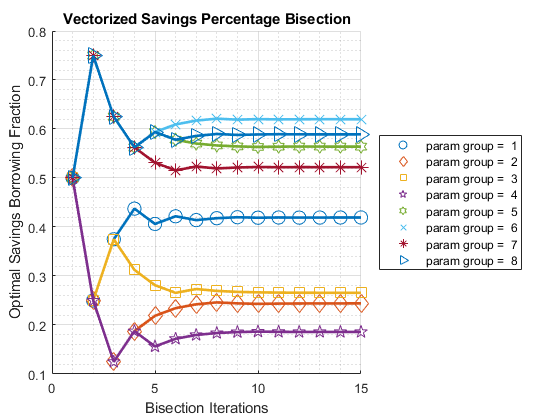
\includegraphics[width=5.20833in,height=\textheight]{img/fx_optim_bisec_savezrone_images/figure_0.png}

\begin{verbatim}
----------------------------------------
xxxxxxxxxxxxxxxxxxxxxxxxxxxxxxxxxxxxxxxx
CONTAINER NAME: mp_container_map ND Array (Matrix etc)
xxxxxxxxxxxxxxxxxxxxxxxxxxxxxxxxxxxxxxxx
                         i    idx    ndim    numel    rowN    colN       sum           mean          std        coefvari        min           max    
                         _    ___    ____    _____    ____    ____    __________    __________    __________    ________    ___________    __________

    ar_opti_foc_obj      1     1      2        8       1       8      0.00050535    6.3168e-05    9.4141e-05     1.4903     -0.00013343    0.00015981
    ar_opti_save_frac    2     2      2        8       1       8            3.41       0.42626       0.17279    0.40536         0.18583        0.6199

xxx TABLE:ar_opti_foc_obj xxxxxxxxxxxxxxxxxx
              c1            c2            c3            c4            c5             c6            c7            c8    
          __________    __________    __________    __________    ___________    __________    __________    __________

    r1    8.1766e-05    3.0909e-05    0.00014822    7.9241e-05    -0.00013343    0.00015981    1.8966e-05    0.00011986

xxx TABLE:ar_opti_save_frac xxxxxxxxxxxxxxxxxx
            c1        c2         c3         c4         c5         c6       c7        c8   
          ______    _______    _______    _______    _______    ______    _____    _______

    r1    0.4194    0.24412    0.26566    0.18583    0.56406    0.6199    0.522    0.58908
\end{verbatim}

\hypertarget{test-ff_optim_bisec_savezrone-one-individual}{%
\subsection{Test FF\_OPTIM\_BISEC\_SAVEZRONE One Individual}\label{test-ff_optim_bisec_savezrone-one-individual}}

Bisection for savings choice at one state:

\begin{verbatim}
% Generate the state-space and function
[fl_z1, fl_z2, fl_r, fl_beta] = deal(0.4730, 0.6252, 0.0839, 0.7365);
% ffi_intertemporal_max is a function in ff_optim_bisec_savezrone for testing
fc_deri_wth_uniroot = @(x) ffi_intertemporal_max(x, fl_z1, fl_z2, fl_r, fl_beta);
% Call Function
bl_verbose = true;
ff_optim_bisec_savezrone(fc_deri_wth_uniroot, bl_verbose);

BISECT END: iteration=16, norm(ar_mid_fx)=0.00016724
                  vartype    paramgroup2
                  _______    ___________

    a             "init"           1e-05
    b             "init"         0.99999
    f_a           "init"           70155
    f_b           "init"          -95255
    it1_fp        "fatx"          -0.502
    it1_p         "x"                0.5
    it2_fp        "fatx"          1.5361
    it2_p         "x"               0.25
    it3_fp        "fatx"         0.34671
    it3_p         "x"              0.375
    it4_fp        "fatx"       -0.089881
    it4_p         "x"             0.4375
    it5_fp        "fatx"         0.12259
    it5_p         "x"            0.40625
    it6_fp        "fatx"        0.015276
    it6_p         "x"            0.42188
    it7_fp        "fatx"       -0.037529
    it7_p         "x"            0.42969
    it8_fp        "fatx"       -0.011188
    it8_p         "x"            0.42578
    it9_fp        "fatx"       0.0020277
    it9_p         "x"            0.42383
    it10_fp       "fatx"      -0.0045843
    it10_p        "x"            0.42481
    it11_fp       "fatx"      -0.0012793
    it11_p        "x"            0.42432
    it12_fp       "fatx"      0.00037392
    it12_p        "x"            0.42407
    it13_fp       "fatx"     -0.00045276
    it13_p        "x"             0.4242
    it14_fp       "fatx"     -3.9436e-05
    it14_p        "x"            0.42413
    it15_fp       "fatx"      0.00016724
    it15_p        "x"             0.4241
    it15_level    "level"       -0.13158
\end{verbatim}

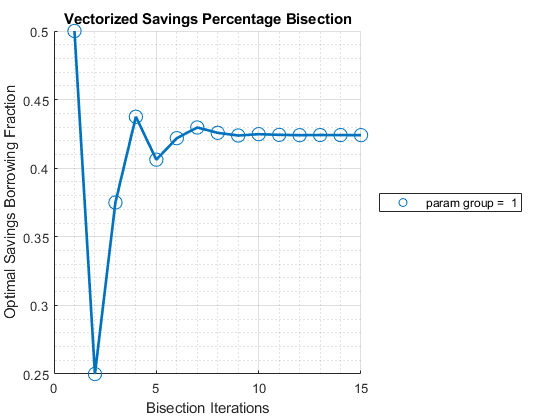
\includegraphics[width=5.20833in,height=\textheight]{img/fx_optim_bisec_savezrone_images/figure_1.png}

\begin{verbatim}
----------------------------------------
xxxxxxxxxxxxxxxxxxxxxxxxxxxxxxxxxxxxxxxx
CONTAINER NAME: mp_container_map Scalars
xxxxxxxxxxxxxxxxxxxxxxxxxxxxxxxxxxxxxxxx
                         i    idx      value   
                         _    ___    __________

    ar_opti_foc_obj      1     1     0.00016724
    ar_opti_save_frac    2     2         0.4241
\end{verbatim}

\hypertarget{test-ff_optim_bisec_savezrone-six-individual-states}{%
\subsection{Test FF\_OPTIM\_BISEC\_SAVEZRONE Six Individual States}\label{test-ff_optim_bisec_savezrone-six-individual-states}}

Solve the two period intertemporal optimization problem with only 6
individual states:

\begin{verbatim}
% Generate the state-space and function
ar_z1 = [1,2,3]';
ar_z2 = [3,2,1]';
ar_r = [1.05, 1.50, 1.30]';
ar_beta = [0.80, 0.95, 1.50]';
mt_fc_inputs = [ar_z1, ar_z2, ar_r, ar_beta];
% ffi_intertemporal_max is a function in ff_optim_bisec_savezrone for testing
fc_deri_wth_uniroot = @(x) ffi_intertemporal_max(x, ar_z1, ar_z2, ar_r, ar_beta);
% Call Function
bl_verbose = true;
ff_optim_bisec_savezrone(fc_deri_wth_uniroot, bl_verbose);

BISECT END: iteration=16, norm(ar_mid_fx)=8.9847e-05
                  vartype    paramgroup2    paramgroup3    paramgroup4
                  _______    ___________    ___________    ___________

    a             "init"           1e-05          1e-05          1e-05
    b             "init"         0.99999        0.99999        0.99999
    f_a           "init"           32475          33928          43671
    f_b           "init"          -40594         -35714         -29113
    it1_fp        "fatx"        -0.16238      -0.035714        0.29114
    it1_p         "x"                0.5            0.5            0.5
    it2_fp        "fatx"         0.75773        0.88092       -0.58225
    it2_p         "x"               0.25           0.25        0.74999
    it3_fp        "fatx"         0.21649        0.33333      -0.077629
    it3_p         "x"              0.375          0.375          0.625
    it4_fp        "fatx"        0.020615        0.14059        0.11091
    it4_p         "x"             0.4375         0.4375         0.5625
    it5_fp        "fatx"        -0.07132       0.051539       0.018865
    it5_p         "x"            0.46875        0.46875        0.59375
    it6_fp        "fatx"       -0.025599      0.0078193      -0.028659
    it6_p         "x"            0.45313        0.48438        0.60937
    it7_fp        "fatx"      -0.0025711      -0.013955     -0.0047386
    it7_p         "x"            0.44531        0.49219        0.60156
    it8_fp        "fatx"       0.0090001     -0.0030715      0.0071001
    it8_p         "x"            0.44141        0.48828        0.59765
    it9_fp        "fatx"       0.0032093      0.0023727      0.0011903
    it9_p         "x"            0.44336        0.48633        0.59961
    it10_fp       "fatx"      0.00031783    -0.00034971     -0.0017717
    it10_p        "x"            0.44434         0.4873        0.60058
    it11_fp       "fatx"      -0.0011269      0.0010114    -0.00029011
    it11_p        "x"            0.44483        0.48682         0.6001
    it12_fp       "fatx"     -0.00040464     0.00033083     0.00045024
    it12_p        "x"            0.44458        0.48706        0.59985
    it13_fp       "fatx"     -4.3425e-05    -9.4396e-06     8.0103e-05
    it13_p        "x"            0.44446        0.48718        0.59997
    it14_fp       "fatx"       0.0001372      0.0001607      -0.000105
    it14_p        "x"             0.4444        0.48712        0.60003
    it15_fp       "fatx"      4.6884e-05     7.5628e-05    -1.2444e-05
    it15_p        "x"            0.44443        0.48715            0.6
    it15_level    "level"        -0.3686        0.56403         1.6261
\end{verbatim}

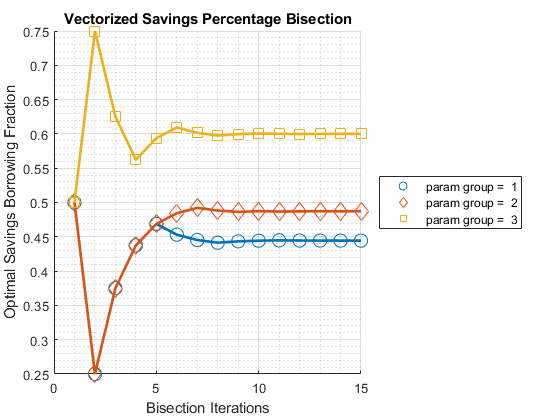
\includegraphics[width=5.20833in,height=\textheight]{img/fx_optim_bisec_savezrone_images/figure_2.png}

\begin{verbatim}
----------------------------------------
xxxxxxxxxxxxxxxxxxxxxxxxxxxxxxxxxxxxxxxx
CONTAINER NAME: mp_container_map ND Array (Matrix etc)
xxxxxxxxxxxxxxxxxxxxxxxxxxxxxxxxxxxxxxxx
                         i    idx    ndim    numel    rowN    colN       sum           mean          std        coefvari        min           max    
                         _    ___    ____    _____    ____    ____    __________    __________    __________    ________    ___________    __________

    ar_opti_foc_obj      1     1      2        3       1       3      0.00011007    3.6689e-05    4.4913e-05     1.2241     -1.2444e-05    7.5628e-05
    ar_opti_save_frac    2     2      2        3       1       3          1.5316       0.51053      0.080379    0.15744         0.44443           0.6

xxx TABLE:ar_opti_foc_obj xxxxxxxxxxxxxxxxxx
              c1            c2            c3     
          __________    __________    ___________

    r1    4.6884e-05    7.5628e-05    -1.2444e-05

xxx TABLE:ar_opti_save_frac xxxxxxxxxxxxxxxxxx
            c1         c2       c3 
          _______    _______    ___

    r1    0.44443    0.48715    0.6
\end{verbatim}

\hypertarget{test-ff_optim_bisec_savezrone-speed}{%
\subsection{Test FF\_OPTIM\_BISEC\_SAVEZRONE Speed}\label{test-ff_optim_bisec_savezrone-speed}}

Test Speed doing 6.25 million bisections for a savings problem:

\begin{verbatim}
% Generate the state-space and function
rng(123);
it_draws = 6250000; % must be even number
ar_z1 = exp(rand([it_draws,1])*3-1.5);
ar_z2 = exp(rand([it_draws,1])*3-1.5);
ar_r = (rand(it_draws,1)*10.0);
ar_beta = [rand(round(it_draws/2),1)*0.9+0.1; rand(round(it_draws/2),1)*0.9+1]; 
% ffi_intertemporal_max is a function in ff_optim_bisec_savezrone for testing
fc_deri_wth_uniroot = @(x) ffi_intertemporal_max(x, ar_z1, ar_z2, ar_r, ar_beta);
% Call Function
bl_verbose = false;
bl_timer = true;
[ar_opti_save_frac, ar_opti_save_level] = ff_optim_bisec_savezrone(fc_deri_wth_uniroot, bl_verbose, bl_timer);

Elapsed time is 3.908350 seconds.

mp_container_map = containers.Map('KeyType','char', 'ValueType','any');
mp_container_map('ar_opti_save_frac') = ar_opti_save_frac;
mp_container_map('ar_opti_save_level') = ar_opti_save_level;
mp_container_map('ar_opti_save_frac_notnan') = ar_opti_save_frac(~isnan(ar_opti_save_frac));
ff_container_map_display(mp_container_map);

----------------------------------------
xxxxxxxxxxxxxxxxxxxxxxxxxxxxxxxxxxxxxxxx
CONTAINER NAME: mp_container_map ND Array (Matrix etc)
xxxxxxxxxxxxxxxxxxxxxxxxxxxxxxxxxxxxxxxx
                                i    idx    ndim     numel        rowN      colN       sum         mean        std      coefvari      min        max  
                                _    ___    ____    ________    ________    ____    __________    _______    _______    ________    _______    _______

    ar_opti_save_frac           1     1      2      6.25e+06    6.25e+06     1       2.884e+06    0.46144    0.15306    0.33171     0.09092    0.65518
    ar_opti_save_frac_notnan    2     2      2      6.25e+06    6.25e+06     1       2.884e+06    0.46144    0.15306    0.33171     0.09092    0.65518
    ar_opti_save_level          3     3      2      6.25e+06    6.25e+06     1      2.9482e+06    0.47172    0.66667     1.4133     -3.9805     2.9221

figure();
histogram(ar_opti_save_frac(~isnan(ar_opti_save_frac)),100);
title('Distribution of Optimal Savings Fractions');
xlabel('Savings Fractions');
grid on;
\end{verbatim}

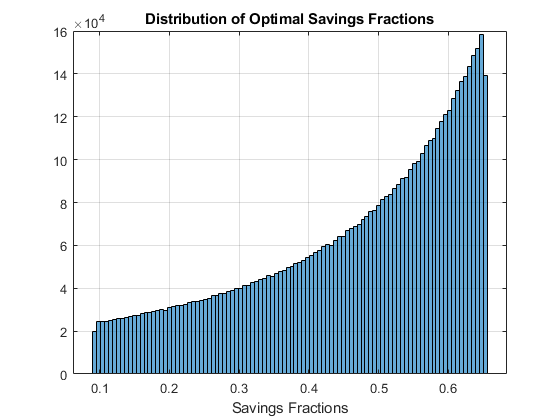
\includegraphics[width=5.20833in,height=\textheight]{img/fx_optim_bisec_savezrone_images/figure_3.png}

\hypertarget{define-two-period-intertemporal-foc-log-utility-no-shock}{%
\subsection{Define Two Period Intertemporal FOC Log Utility No Shock}\label{define-two-period-intertemporal-foc-log-utility-no-shock}}

See \href{https://fanwangecon.github.io/Math4Econ/derivative_application/htmlpdfm/K_save_households.html}{Household's Utility Maximization Problem and Two-Period Borrowing
and Savings Problem given
Endowments}.

\begin{verbatim}
function [ar_deri_zero, ar_saveborr_level] = ffi_intertemporal_max(ar_saveborr_frac, z1, z2, r, beta)
    ar_saveborr_level = ar_saveborr_frac.*(z1+z2./(1+r)) - z2./(1+r);
    ar_deri_zero = 1./(ar_saveborr_level-z1) + (beta.*(r+1))./(z2 + ar_saveborr_level.*(r+1));
end
\end{verbatim}

\hypertarget{ff_optim_mlsec_savezrone-derivative-multisection}{%
\section{FF\_OPTIM\_MLSEC\_SAVEZRONE Derivative Multisection}\label{ff_optim_mlsec_savezrone-derivative-multisection}}

\begin{quote}
Go back to \href{http://fanwangecon.github.io/}{fan}'s \href{https://fanwangecon.github.io/MEconTools/}{MEconTools} Toolbox (\href{https://fanwangecon.github.io/MEconTools/bookdown}{bookdown}), \href{https://fanwangecon.github.io/M4Econ/}{Matlab Code Examples} Repository (\href{https://fanwangecon.github.io/M4Econ/bookdown}{bookdown}), or \href{https://fanwangecon.github.io/Math4Econ/}{Math for Econ with Matlab} Repository (\href{https://fanwangecon.github.io/Math4Econ/bookdown}{bookdown}).
\end{quote}

This is the example vignette for function:
\href{https://github.com/FanWangEcon//MEconTools/blob/master/MEconTools/optim/ff_optim_mlsec_savezrone.m}{\textbf{ff\_optim\_mlsec\_savezrone}}
from the \href{https://fanwangecon.github.io/MEconTools/}{\textbf{MEconTools
Package}}\textbf{.} This
functions solves for optimal savings/borrowing level given an anonymous
function that provides the derivative of a intertemporal savings
problem. This is a vectorized function solved with multi-section
(multiple points bisection concurrently).

The vectorized and looped bisection savings problem rely on this
function to solve for optimal savings choices:

\begin{itemize}
\item
  States Grid + Continuous Exact Savings as Share of Cash-on-Hand :\href{https://github.com/FanWangEcon/MEconTools/blob/master/MEconTools/vfi/ff_vfi_az_bisec_loop.m}{\textbf{ff\_vfi\_az\_bisec\_loop}},
  high precision even with small grid
\item
  States Grid + Continuous Exact Savings as Share of Cash-on-Hand :
  \href{https://github.com/FanWangEcon/MEconTools/blob/master/MEconTools/vfi/ff_vfi_az_bisec_vec.m}{\textbf{ff\_vfi\_az\_bisec\_vec}},
  precision and speed
\end{itemize}

\hypertarget{test-ff_optim_mlsec_savezrone-one-individual}{%
\subsection{Test FF\_OPTIM\_MLSEC\_SAVEZRONE One Individual}\label{test-ff_optim_mlsec_savezrone-one-individual}}

Bisection for savings choice at one state:

\begin{verbatim}
% Generate the state-space and function
[fl_z1, fl_z2, fl_r, fl_beta] = deal(0.4730, 0.6252, 0.0839, 0.7365);
% ffi_intertemporal_max is a function in ff_optim_mlsec_savezrone for testing
fc_deri_wth_uniroot = @(x) ffi_intertemporal_max(x, fl_z1, fl_z2, fl_r, fl_beta);
% Call Function
bl_verbose = false;
bl_timer = true;
% optimally borrowing given the parameters here
mp_mlsec_ctrlinfo = containers.Map('KeyType','char', 'ValueType','any');
mp_mlsec_ctrlinfo('it_mzoom_jnt_pnts') = 10;
mp_mlsec_ctrlinfo('it_mzoom_max_iter') = 4;
[fl_opti_save_frac, fl_opti_save_level] = ...
    ff_optim_mlsec_savezrone(fc_deri_wth_uniroot, bl_verbose, bl_timer, mp_mlsec_ctrlinfo)

Elapsed time is 0.002805 seconds.
fl_opti_save_frac = 0.4241
fl_opti_save_level = -0.1316
\end{verbatim}

\hypertarget{test-ff_optim_mlsec_savezrone-5-individuals-5-iterations-5-points-per-iteration}{%
\subsection{Test FF\_OPTIM\_MLSEC\_SAVEZRONE 5 Individuals 5 Iterations 5 Points Per Iteration}\label{test-ff_optim_mlsec_savezrone-5-individuals-5-iterations-5-points-per-iteration}}

5 grid points per iteration, and 5 iterations.

\begin{verbatim}
% Generate the state-space and function
rng(123);
it_draws = 6; % must be even number
ar_z1 = exp(rand([it_draws,1])*3-1.5);
ar_z2 = exp(rand([it_draws,1])*3-1.5);
ar_r = (rand(it_draws,1)*10.0);
ar_beta = [rand(round(it_draws/2),1)*0.9+0.1; rand(round(it_draws/2),1)*0.9+1]; 
fc_deri_wth_uniroot = @(x) ffi_intertemporal_max(x, ar_z1, ar_z2, ar_r, ar_beta);
% Call Function
bl_verbose = true;
bl_timer = true;
mp_mlsec_ctrlinfo = containers.Map('KeyType','char', 'ValueType','any');
mp_mlsec_ctrlinfo('it_mlsect_jnt_pnts') = 5;
mp_mlsec_ctrlinfo('it_mlsect_max_iter') = 5;
ff_optim_mlsec_savezrone(fc_deri_wth_uniroot, bl_verbose, bl_timer, mp_mlsec_ctrlinfo);

    iter    cl_row_names_a     Var1       Var2       Var3       Var4       Var5       Var6  
    ____    ______________    _______    _______    _______    _______    _______    _______

     0        "point=1"         1e-05      1e-05      1e-05      1e-05      1e-05      1e-05
     1        "point=1"         1e-05      1e-05      1e-05      1e-05      1e-05      1e-05
     1        "point=2"       0.25001    0.25001    0.25001    0.25001    0.25001    0.25001
     1        "point=3"           0.5        0.5        0.5        0.5        0.5        0.5
     1        "point=4"          0.75       0.75       0.75       0.75       0.75       0.75
     1        "point=5"       0.99999    0.99999    0.99999    0.99999    0.99999    0.99999
     2        "point=1"       0.29167    0.29167    0.29167    0.54167    0.54167    0.54167
     2        "point=2"       0.33334    0.33334    0.33334    0.58333    0.58333    0.58333
     2        "point=3"         0.375      0.375      0.375      0.625      0.625      0.625
     2        "point=4"       0.41667    0.41667    0.41667    0.66666    0.66666    0.66666
     2        "point=5"       0.45833    0.45833    0.45833    0.70833    0.70833    0.70833
     3        "point=1"       0.34028    0.34028    0.38195    0.63194    0.59028    0.59028
     3        "point=2"       0.34723    0.34723    0.38889    0.63889    0.59722    0.59722
     3        "point=3"       0.35417    0.35417    0.39584    0.64583    0.60416    0.60416
     3        "point=4"       0.36111    0.36111    0.40278    0.65277    0.61111    0.61111
     3        "point=5"       0.36806    0.36806    0.40972    0.65972    0.61805    0.61805
     4        "point=1"       0.36227    0.36227    0.39699     0.6331    0.61921    0.60532
     4        "point=2"       0.36343    0.36343    0.39815    0.63426    0.62037    0.60648
     4        "point=3"       0.36459    0.36459    0.39931    0.63541    0.62153    0.60764
     4        "point=4"       0.36574    0.36574    0.40046    0.63657    0.62268    0.60879
     4        "point=5"        0.3669     0.3669    0.40162    0.63773    0.62384    0.60995
     5        "point=1"       0.36594    0.36594    0.40066    0.63792    0.62288    0.60783
     5        "point=2"       0.36613    0.36613    0.40085    0.63811    0.62307    0.60802
     5        "point=3"       0.36632    0.36632    0.40104    0.63831    0.62326    0.60822
     5        "point=4"       0.36652    0.36652    0.40124     0.6385    0.62345    0.60841
     5        "point=5"       0.36671    0.36671    0.40143    0.63869    0.62365     0.6086
\end{verbatim}

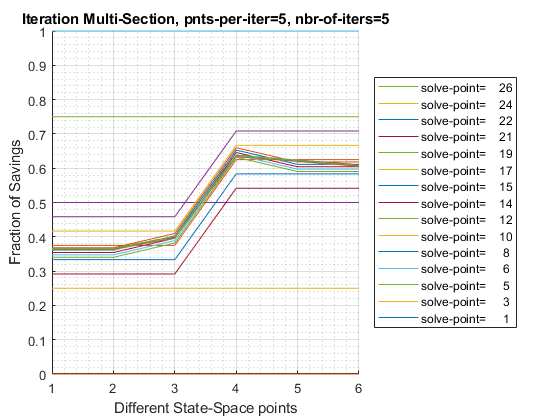
\includegraphics[width=5.20833in,height=\textheight]{img/fx_optim_mlsec_savezrone_images/figure_0.png}

\begin{verbatim}
Elapsed time is 0.406584 seconds.
----------------------------------------
xxxxxxxxxxxxxxxxxxxxxxxxxxxxxxxxxxxxxxxx
CONTAINER NAME: mp_container_map ND Array (Matrix etc)
xxxxxxxxxxxxxxxxxxxxxxxxxxxxxxxxxxxxxxxx
                         i    idx    ndim    numel    rowN    colN        sum           mean           std        coefvari        min           max    
                         _    ___    ____    _____    ____    ____    ___________    ___________    __________    ________    ___________    __________

    ar_opti_foc_obj      1     1      2        6       6       1      -0.00037648    -6.2746e-05    0.00042601    -6.7894     -0.00067107    0.00055875
    ar_opti_save_frac    2     2      2        6       6       1           3.0037        0.50061       0.13506    0.26979         0.36642       0.63821

xxx TABLE:ar_opti_foc_obj xxxxxxxxxxxxxxxxxx
              c1     
          ___________

    r1     7.0837e-05
    r2     -0.0002782
    r3     0.00017713
    r4     0.00055875
    r5    -0.00023392
    r6    -0.00067107

xxx TABLE:ar_opti_save_frac xxxxxxxxxxxxxxxxxx
            c1   
          _______

    r1    0.36642
    r2    0.36661
    r3    0.40153
    r4    0.63821
    r5    0.62297
    r6    0.60793
\end{verbatim}

\hypertarget{test-ff_optim_mlsec_savezrone-8-individuals-3-iterations-10-points-per-iteration}{%
\subsection{Test FF\_OPTIM\_MLSEC\_SAVEZRONE 8 Individuals 3 Iterations 10 Points Per Iteration}\label{test-ff_optim_mlsec_savezrone-8-individuals-3-iterations-10-points-per-iteration}}

10 grid points per iteration, and 3 iterations.

\begin{verbatim}
% Generate the state-space and function
rng(123);
it_draws = 8; % must be even number
ar_z1 = exp(rand([it_draws,1])*3-1.5);
ar_z2 = exp(rand([it_draws,1])*3-1.5);
ar_r = (rand(it_draws,1)*10.0);
ar_beta = [rand(round(it_draws/2),1)*0.9+0.1; rand(round(it_draws/2),1)*0.9+1]; 
fc_deri_wth_uniroot = @(x) ffi_intertemporal_max(x, ar_z1, ar_z2, ar_r, ar_beta);
% Call Function
bl_verbose = true;
bl_timer = true;
mp_mlsec_ctrlinfo = containers.Map('KeyType','char', 'ValueType','any');
mp_mlsec_ctrlinfo('it_mlsect_jnt_pnts') = 10;
mp_mlsec_ctrlinfo('it_mlsect_max_iter') = 3;
ff_optim_mlsec_savezrone(fc_deri_wth_uniroot, bl_verbose, bl_timer, mp_mlsec_ctrlinfo);

    iter    cl_row_names_a     Var1       Var2       Var3       Var4       Var5       Var6       Var7       Var8  
    ____    ______________    _______    _______    _______    _______    _______    _______    _______    _______

     0        "point=1"         1e-05      1e-05      1e-05      1e-05      1e-05      1e-05      1e-05      1e-05
     1        "point=1"         1e-05      1e-05      1e-05      1e-05      1e-05      1e-05      1e-05      1e-05
     1        "point=2"       0.11112    0.11112    0.11112    0.11112    0.11112    0.11112    0.11112    0.11112
     1        "point=3"       0.22223    0.22223    0.22223    0.22223    0.22223    0.22223    0.22223    0.22223
     1        "point=4"       0.33334    0.33334    0.33334    0.33334    0.33334    0.33334    0.33334    0.33334
     1        "point=5"       0.44445    0.44445    0.44445    0.44445    0.44445    0.44445    0.44445    0.44445
     1        "point=6"       0.55555    0.55555    0.55555    0.55555    0.55555    0.55555    0.55555    0.55555
     1        "point=7"       0.66666    0.66666    0.66666    0.66666    0.66666    0.66666    0.66666    0.66666
     1        "point=8"       0.77777    0.77777    0.77777    0.77777    0.77777    0.77777    0.77777    0.77777
     1        "point=9"       0.88888    0.88888    0.88888    0.88888    0.88888    0.88888    0.88888    0.88888
     1        "point=10"      0.99999    0.99999    0.99999    0.99999    0.99999    0.99999    0.99999    0.99999
     2        "point=1"       0.34344    0.23233    0.23233    0.23233    0.56566    0.56566    0.45455    0.56566
     2        "point=2"       0.35354    0.24243    0.24243    0.24243    0.57576    0.57576    0.46465    0.57576
     2        "point=3"       0.36364    0.25253    0.25253    0.25253    0.58586    0.58586    0.47475    0.58586
     2        "point=4"       0.37374    0.26263    0.26263    0.26263    0.59596    0.59596    0.48485    0.59596
     2        "point=5"       0.38384    0.27273    0.27273    0.27273    0.60606    0.60606    0.49495    0.60606
     2        "point=6"       0.39394    0.28283    0.28283    0.28283    0.61616    0.61616    0.50505    0.61616
     2        "point=7"       0.40404    0.29293    0.29293    0.29293    0.62626    0.62626    0.51515    0.62626
     2        "point=8"       0.41414    0.30303    0.30303    0.30303    0.63636    0.63636    0.52525    0.63636
     2        "point=9"       0.42424    0.31314    0.31314    0.31314    0.64646    0.64646    0.53535    0.64646
     2        "point=10"      0.43434    0.32324    0.32324    0.32324    0.65656    0.65656    0.54545    0.65656
     3        "point=1"       0.42516    0.27365    0.29385    0.23325    0.55647    0.60698    0.51607    0.57667
     3        "point=2"       0.42608    0.27457    0.29477    0.23417    0.55739    0.60789    0.51699    0.57759
     3        "point=3"         0.427    0.27549    0.29569    0.23508    0.55831    0.60881    0.51791    0.57851
     3        "point=4"       0.42792     0.2764    0.29661      0.236    0.55923    0.60973    0.51882    0.57943
     3        "point=5"       0.42884    0.27732    0.29752    0.23692    0.56015    0.61065    0.51974    0.58035
     3        "point=6"       0.42975    0.27824    0.29844    0.23784    0.56106    0.61157    0.52066    0.58127
     3        "point=7"       0.43067    0.27916    0.29936    0.23876    0.56198    0.61249    0.52158    0.58218
     3        "point=8"       0.43159    0.28008    0.30028    0.23967     0.5629     0.6134     0.5225     0.5831
     3        "point=9"       0.43251      0.281     0.3012    0.24059    0.56382    0.61432    0.52342    0.58402
     3        "point=10"      0.43343    0.28191    0.30212    0.24151    0.56474    0.61524    0.52433    0.58494
\end{verbatim}

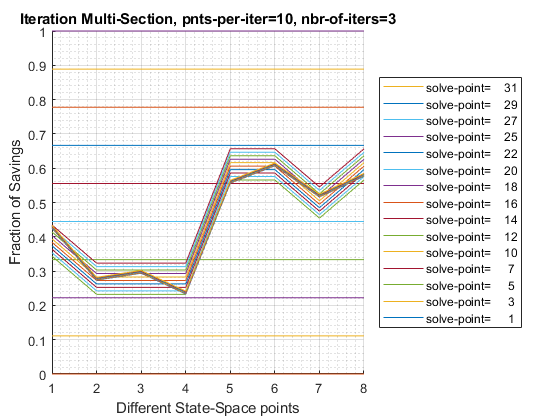
\includegraphics[width=5.20833in,height=\textheight]{img/fx_optim_mlsec_savezrone_images/figure_1.png}

\begin{verbatim}
Elapsed time is 0.633499 seconds.
----------------------------------------
xxxxxxxxxxxxxxxxxxxxxxxxxxxxxxxxxxxxxxxx
CONTAINER NAME: mp_container_map ND Array (Matrix etc)
xxxxxxxxxxxxxxxxxxxxxxxxxxxxxxxxxxxxxxxx
                         i    idx    ndim    numel    rowN    colN       sum          mean          std       coefvari       min           max   
                         _    ___    ____    _____    ____    ____    _________    __________    _________    ________    __________    _________

    ar_opti_foc_obj      1     1      2        8       8       1      0.0033175    0.00041468    0.0029592     7.1361     -0.0044871    0.0050249
    ar_opti_save_frac    2     2      2        8       8       1         3.5124       0.43905      0.15005    0.34177        0.23371      0.61019

xxx TABLE:ar_opti_foc_obj xxxxxxxxxxxxxxxxxx
              c1     
          ___________

    r1     0.00087102
    r2      0.0033354
    r3     -0.0044871
    r4       0.001317
    r5     -0.0017862
    r6      0.0050249
    r7    -0.00058496
    r8    -0.00037273

xxx TABLE:ar_opti_save_frac xxxxxxxxxxxxxxxxxx
            c1   
          _______

    r1    0.42838
    r2    0.28054
    r3     0.2989
    r4    0.23371
    r5    0.55877
    r6    0.61019
    r7     0.5202
    r8    0.58172
\end{verbatim}

\hypertarget{test-ff_optim_mlsec_savezrone-speed}{%
\subsection{Test FF\_OPTIM\_MLSEC\_SAVEZRONE Speed}\label{test-ff_optim_mlsec_savezrone-speed}}

Test Speed doing 6.25 million multisections for a savings problem:

\begin{verbatim}
% Generate the state-space and function
rng(123);
it_draws = 6250000; % must be even number
ar_z1 = exp(rand([it_draws,1])*3-1.5);
ar_z2 = exp(rand([it_draws,1])*3-1.5);
ar_r = (rand(it_draws,1)*10.0);
ar_beta = [rand(round(it_draws/2),1)*0.9+0.1; rand(round(it_draws/2),1)*0.9+1]; 
% ffi_intertemporal_max is a function in ff_optim_mlsec_savezrone for testing
fc_deri_wth_uniroot = @(x) ffi_intertemporal_max(x, ar_z1, ar_z2, ar_r, ar_beta);
% Call Function
bl_verbose = false;
bl_timer = true;
[ar_opti_save_frac, ar_opti_save_level] = ff_optim_mlsec_savezrone(fc_deri_wth_uniroot, bl_verbose, bl_timer);

Elapsed time is 13.672896 seconds.

mp_container_map = containers.Map('KeyType','char', 'ValueType','any');
mp_container_map('ar_opti_save_frac') = ar_opti_save_frac;
mp_container_map('ar_opti_save_level') = ar_opti_save_level;
mp_container_map('ar_opti_save_frac_notnan') = ar_opti_save_frac(~isnan(ar_opti_save_frac));
ff_container_map_display(mp_container_map);

----------------------------------------
xxxxxxxxxxxxxxxxxxxxxxxxxxxxxxxxxxxxxxxx
CONTAINER NAME: mp_container_map ND Array (Matrix etc)
xxxxxxxxxxxxxxxxxxxxxxxxxxxxxxxxxxxxxxxx
                                i    idx    ndim     numel        rowN      colN       sum         mean        std      coefvari      min         max  
                                _    ___    ____    ________    ________    ____    __________    _______    _______    ________    ________    _______

    ar_opti_save_frac           1     1      2      6.25e+06    6.25e+06     1       2.884e+06    0.46144    0.15306    0.33171     0.090876    0.65519
    ar_opti_save_frac_notnan    2     2      2      6.25e+06    6.25e+06     1       2.884e+06    0.46144    0.15306    0.33171     0.090876    0.65519
    ar_opti_save_level          3     3      2      6.25e+06    6.25e+06     1      2.9482e+06    0.47172    0.66667     1.4133      -3.9807      2.922

figure();
histogram(ar_opti_save_frac(~isnan(ar_opti_save_frac)),100);
title('Distribution of Optimal Savings Fractions');
xlabel('Savings Fractions');
grid on;
\end{verbatim}

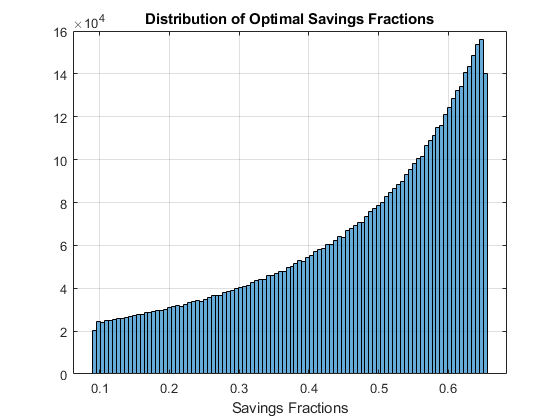
\includegraphics[width=5.20833in,height=\textheight]{img/fx_optim_mlsec_savezrone_images/figure_2.png}

\hypertarget{define-two-period-intertemporal-foc-log-utility-no-shock-1}{%
\subsection{Define Two Period Intertemporal FOC Log Utility No Shock}\label{define-two-period-intertemporal-foc-log-utility-no-shock-1}}

See \href{https://fanwangecon.github.io/Math4Econ/derivative_application/htmlpdfm/K_save_households.html}{Household's Utility Maximization Problem and Two-Period Borrowing
and Savings Problem given
Endowments}.

\begin{verbatim}
function [ar_deri_zero, ar_saveborr_level] = ffi_intertemporal_max(ar_saveborr_frac, z1, z2, r, beta)
    ar_saveborr_level = ar_saveborr_frac.*(z1+z2./(1+r)) - z2./(1+r);
    ar_deri_zero = 1./(ar_saveborr_level-z1) + (beta.*(r+1))./(z2 + ar_saveborr_level.*(r+1));
end
\end{verbatim}

\hypertarget{ff_optim_mzoom_savezrone-derivative-multisection}{%
\section{FF\_OPTIM\_MZOOM\_SAVEZRONE Derivative Multisection}\label{ff_optim_mzoom_savezrone-derivative-multisection}}

\begin{quote}
Go back to \href{http://fanwangecon.github.io/}{fan}'s \href{https://fanwangecon.github.io/MEconTools/}{MEconTools} Toolbox (\href{https://fanwangecon.github.io/MEconTools/bookdown}{bookdown}), \href{https://fanwangecon.github.io/M4Econ/}{Matlab Code Examples} Repository (\href{https://fanwangecon.github.io/M4Econ/bookdown}{bookdown}), or \href{https://fanwangecon.github.io/Math4Econ/}{Math for Econ with Matlab} Repository (\href{https://fanwangecon.github.io/Math4Econ/bookdown}{bookdown}).
\end{quote}

This is the example vignette for function:
\href{https://github.com/FanWangEcon//MEconTools/blob/master/MEconTools/optim/ff_optim_mzoom_savezrone.m}{\textbf{ff\_optim\_mzoom\_savezrone}}
from the \href{https://fanwangecon.github.io/MEconTools/}{\textbf{MEconTools
Package}}\textbf{.} This
functions solves for optimal savings/borrowing level given an anonymous
function that provides the utility (not derivative) of a intertemporal
savings problem. This is a vectorized function solves for multiple
state-space elements at the same time. The function allows for controls
of iteration counts, the number of evaluations per iteration, and how
much to "zoom-in" for each iteration around the last iteration's
maximum/optimal choice.

Note that if first order conditions are available this method should not
be used, but
\href{https://github.com/FanWangEcon//MEconTools/blob/master/MEconTools/optim/ff_optim_mlsec_savezrone.m}{\textbf{ff\_optim\_mlsec\_savezrone}}
should be used.
\href{https://github.com/FanWangEcon//MEconTools/blob/master/MEconTools/optim/ff_optim_mlsec_savezrone.m}{\textbf{ff\_optim\_mlsec\_savezrone}}
relies on bisection. In the first example below more values are needed
to achieve the same precision than under
\href{https://github.com/FanWangEcon//MEconTools/blob/master/MEconTools/optim/ff_optim_mlsec_savezrone.m}{\textbf{ff\_optim\_mlsec\_savezrone}}\textbf{.}
However, increasing might not expensive given vectorization, should
increase time cost linearly in generally. MZOOM is much more robust than
bisection based methods. And by increasing the number of points
evaluated per iteration, in limited number of iterations, the
approximately exact optimal savings choice can be found.

The vectorized zooming savings problem rely on this function to solve
for optimal savings choices:

\begin{itemize}
\tightlist
\item
  States Grid + Approximate Continuous Exact Savings (zoom) as Share
  of Cash-on-Hand :
  \href{https://github.com/FanWangEcon/MEconTools/blob/master/MEconTools/vfi/ff_vfi_az_zoom_vec.m}{\textbf{ff\_vfi\_az\_zoom\_vec}},
  precision and speed
\end{itemize}

\hypertarget{test-ff_optim_mzoom_savezrone-one-individual}{%
\subsection{Test FF\_OPTIM\_MZOOM\_SAVEZRONE One Individual}\label{test-ff_optim_mzoom_savezrone-one-individual}}

Bisection for savings choice at one state:

\begin{verbatim}
% Generate the state-space and function
[fl_z1, fl_z2, fl_r, fl_beta] = deal(0.4730, 0.6252, 0.0839, 0.7365);
% ffi_intertemporal_max is a function in ff_optim_mlsec_savezrone for testing
fc_util = @(x) ffi_intertemporal_util(x, fl_z1, fl_z2, fl_r, fl_beta);
% Call Function
bl_verbose = false;
bl_timer = true;
% optimally borrowing given the parameters here
mp_mzoom_ctrlinfo = containers.Map('KeyType','char', 'ValueType','any');
mp_mzoom_ctrlinfo('it_mzoom_jnt_pnts') = 15;
mp_mzoom_ctrlinfo('it_mzoom_max_iter') = 10;
mp_mzoom_ctrlinfo('it_mzoom_zm_ratio') = 0.25;
[fl_opti_save_frac, fl_opti_save_level] = ...
    ff_optim_mzoom_savezrone(fc_util, bl_verbose, bl_timer, mp_mzoom_ctrlinfo)

Elapsed time is 0.004395 seconds.
fl_opti_save_frac = 0.4241
fl_opti_save_level = -0.1316
\end{verbatim}

\hypertarget{test-ff_optim_mzoom_savezrone-4-individuals-3-iterations-50-points-per-iteration}{%
\subsection{Test FF\_OPTIM\_MZOOM\_SAVEZRONE 4 Individuals 3 Iterations 50 Points Per Iteration}\label{test-ff_optim_mzoom_savezrone-4-individuals-3-iterations-50-points-per-iteration}}

5 grid points per iteration, and 5 iterations.

\begin{verbatim}
% Generate the state-space and function
rng(123);
it_draws = 4; % must be even number
ar_z1 = exp(rand([it_draws,1])*3-1.5);
ar_z2 = exp(rand([it_draws,1])*3-1.5);
ar_r = (rand(it_draws,1)*10.0);
ar_beta = [rand(round(it_draws/2),1)*0.9+0.1; rand(round(it_draws/2),1)*0.9+1]; 
fc_util = @(x) ffi_intertemporal_util(x, ar_z1, ar_z2, ar_r, ar_beta);
% Call Function
bl_verbose = true;
bl_timer = true;
mp_mzoom_ctrlinfo = containers.Map('KeyType','char', 'ValueType','any');
mp_mzoom_ctrlinfo('it_mzoom_jnt_pnts') = 50;
mp_mzoom_ctrlinfo('it_mzoom_max_iter') = 3;
mp_mzoom_ctrlinfo('it_mzoom_zm_ratio') = 0;
ff_optim_mzoom_savezrone(fc_util, bl_verbose, bl_timer, mp_mzoom_ctrlinfo);

    iter    cl_row_names_a      Var1        Var2        Var3        Var4  
    ____    ______________    ________    ________    ________    ________

     1        "point=1"          1e-05       1e-05       1e-05       1e-05
     1        "point=2"       0.020418    0.020418    0.020418    0.020418
     1        "point=3"       0.040826    0.040826    0.040826    0.040826
     1        "point=4"       0.061233    0.061233    0.061233    0.061233
     1        "point=5"       0.081641    0.081641    0.081641    0.081641
     1        "point=6"        0.10205     0.10205     0.10205     0.10205
     1        "point=7"        0.12246     0.12246     0.12246     0.12246
     1        "point=8"        0.14286     0.14286     0.14286     0.14286
     1        "point=9"        0.16327     0.16327     0.16327     0.16327
     1        "point=10"       0.18368     0.18368     0.18368     0.18368
     1        "point=11"       0.20409     0.20409     0.20409     0.20409
     1        "point=12"        0.2245      0.2245      0.2245      0.2245
     1        "point=13"        0.2449      0.2449      0.2449      0.2449
     1        "point=14"       0.26531     0.26531     0.26531     0.26531
     1        "point=15"       0.28572     0.28572     0.28572     0.28572
     1        "point=16"       0.30613     0.30613     0.30613     0.30613
     1        "point=17"       0.32653     0.32653     0.32653     0.32653
     1        "point=18"       0.34694     0.34694     0.34694     0.34694
     1        "point=19"       0.36735     0.36735     0.36735     0.36735
     1        "point=20"       0.38776     0.38776     0.38776     0.38776
     1        "point=21"       0.40817     0.40817     0.40817     0.40817
     1        "point=22"       0.42857     0.42857     0.42857     0.42857
     1        "point=23"       0.44898     0.44898     0.44898     0.44898
     1        "point=24"       0.46939     0.46939     0.46939     0.46939
     1        "point=25"        0.4898      0.4898      0.4898      0.4898
     1        "point=26"        0.5102      0.5102      0.5102      0.5102
     1        "point=27"       0.53061     0.53061     0.53061     0.53061
     1        "point=28"       0.55102     0.55102     0.55102     0.55102
     1        "point=29"       0.57143     0.57143     0.57143     0.57143
     1        "point=30"       0.59183     0.59183     0.59183     0.59183
     1        "point=31"       0.61224     0.61224     0.61224     0.61224
     1        "point=32"       0.63265     0.63265     0.63265     0.63265
     1        "point=33"       0.65306     0.65306     0.65306     0.65306
     1        "point=34"       0.67347     0.67347     0.67347     0.67347
     1        "point=35"       0.69387     0.69387     0.69387     0.69387
     1        "point=36"       0.71428     0.71428     0.71428     0.71428
     1        "point=37"       0.73469     0.73469     0.73469     0.73469
     1        "point=38"        0.7551      0.7551      0.7551      0.7551
     1        "point=39"        0.7755      0.7755      0.7755      0.7755
     1        "point=40"       0.79591     0.79591     0.79591     0.79591
     1        "point=41"       0.81632     0.81632     0.81632     0.81632
     1        "point=42"       0.83673     0.83673     0.83673     0.83673
     1        "point=43"       0.85714     0.85714     0.85714     0.85714
     1        "point=44"       0.87754     0.87754     0.87754     0.87754
     1        "point=45"       0.89795     0.89795     0.89795     0.89795
     1        "point=46"       0.91836     0.91836     0.91836     0.91836
     1        "point=47"       0.93877     0.93877     0.93877     0.93877
     1        "point=48"       0.95917     0.95917     0.95917     0.95917
     1        "point=49"       0.97958     0.97958     0.97958     0.97958
     1        "point=50"       0.99999     0.99999     0.99999     0.99999
     2        "point=1"        0.30693     0.12326     0.55182     0.61304
     2        "point=2"        0.30773     0.12406     0.55262     0.61384
     2        "point=3"        0.30853     0.12486     0.55342     0.61464
     2        "point=4"        0.30933     0.12566     0.55422     0.61544
     2        "point=5"        0.31013     0.12646     0.55502     0.61624
     2        "point=6"        0.31093     0.12726     0.55582     0.61704
     2        "point=7"        0.31173     0.12806     0.55662     0.61784
     2        "point=8"        0.31253     0.12886     0.55742     0.61865
     2        "point=9"        0.31333     0.12966     0.55822     0.61945
     2        "point=10"       0.31413     0.13046     0.55902     0.62025
     2        "point=11"       0.31493     0.13126     0.55982     0.62105
     2        "point=12"       0.31573     0.13206     0.56062     0.62185
     2        "point=13"       0.31653     0.13286     0.56142     0.62265
     2        "point=14"       0.31733     0.13366     0.56222     0.62345
     2        "point=15"       0.31813     0.13446     0.56302     0.62425
     2        "point=16"       0.31893     0.13526     0.56382     0.62505
     2        "point=17"       0.31973     0.13606     0.56462     0.62585
     2        "point=18"       0.32053     0.13686     0.56542     0.62665
     2        "point=19"       0.32133     0.13766     0.56623     0.62745
     2        "point=20"       0.32213     0.13846     0.56703     0.62825
     2        "point=21"       0.32293     0.13926     0.56783     0.62905
     2        "point=22"       0.32373     0.14006     0.56863     0.62985
     2        "point=23"       0.32453     0.14086     0.56943     0.63065
     2        "point=24"       0.32533     0.14166     0.57023     0.63145
     2        "point=25"       0.32613     0.14246     0.57103     0.63225
     2        "point=26"       0.32693     0.14326     0.57183     0.63305
     2        "point=27"       0.32773     0.14406     0.57263     0.63385
     2        "point=28"       0.32853     0.14487     0.57343     0.63465
     2        "point=29"       0.32934     0.14567     0.57423     0.63545
     2        "point=30"       0.33014     0.14647     0.57503     0.63625
     2        "point=31"       0.33094     0.14727     0.57583     0.63705
     2        "point=32"       0.33174     0.14807     0.57663     0.63785
     2        "point=33"       0.33254     0.14887     0.57743     0.63865
     2        "point=34"       0.33334     0.14967     0.57823     0.63945
     2        "point=35"       0.33414     0.15047     0.57903     0.64025
     2        "point=36"       0.33494     0.15127     0.57983     0.64105
     2        "point=37"       0.33574     0.15207     0.58063     0.64185
     2        "point=38"       0.33654     0.15287     0.58143     0.64265
     2        "point=39"       0.33734     0.15367     0.58223     0.64345
     2        "point=40"       0.33814     0.15447     0.58303     0.64425
     2        "point=41"       0.33894     0.15527     0.58383     0.64506
     2        "point=42"       0.33974     0.15607     0.58463     0.64586
     2        "point=43"       0.34054     0.15687     0.58543     0.64666
     2        "point=44"       0.34134     0.15767     0.58623     0.64746
     2        "point=45"       0.34214     0.15847     0.58703     0.64826
     2        "point=46"       0.34294     0.15927     0.58783     0.64906
     2        "point=47"       0.34374     0.16007     0.58863     0.64986
     2        "point=48"       0.34454     0.16087     0.58943     0.65066
     2        "point=49"       0.34534     0.16167     0.59023     0.65146
     2        "point=50"       0.34614     0.16247     0.59103     0.65226
     3        "point=1"        0.32937     0.13129     0.57426     0.62348
     3        "point=2"         0.3294     0.13132     0.57429     0.62351
     3        "point=3"        0.32943     0.13135     0.57432     0.62354
     3        "point=4"        0.32946     0.13139     0.57435     0.62357
     3        "point=5"        0.32949     0.13142     0.57439      0.6236
     3        "point=6"        0.32952     0.13145     0.57442     0.62364
     3        "point=7"        0.32955     0.13148     0.57445     0.62367
     3        "point=8"        0.32959     0.13151     0.57448      0.6237
     3        "point=9"        0.32962     0.13154     0.57451     0.62373
     3        "point=10"       0.32965     0.13157     0.57454     0.62376
     3        "point=11"       0.32968     0.13161     0.57457     0.62379
     3        "point=12"       0.32971     0.13164      0.5746     0.62382
     3        "point=13"       0.32974     0.13167     0.57464     0.62385
     3        "point=14"       0.32977      0.1317     0.57467     0.62389
     3        "point=15"       0.32981     0.13173      0.5747     0.62392
     3        "point=16"       0.32984     0.13176     0.57473     0.62395
     3        "point=17"       0.32987     0.13179     0.57476     0.62398
     3        "point=18"        0.3299     0.13182     0.57479     0.62401
     3        "point=19"       0.32993     0.13186     0.57482     0.62404
     3        "point=20"       0.32996     0.13189     0.57486     0.62407
     3        "point=21"       0.32999     0.13192     0.57489     0.62411
     3        "point=22"       0.33003     0.13195     0.57492     0.62414
     3        "point=23"       0.33006     0.13198     0.57495     0.62417
     3        "point=24"       0.33009     0.13201     0.57498      0.6242
     3        "point=25"       0.33012     0.13204     0.57501     0.62423
     3        "point=26"       0.33015     0.13208     0.57504     0.62426
     3        "point=27"       0.33018     0.13211     0.57508     0.62429
     3        "point=28"       0.33021     0.13214     0.57511     0.62433
     3        "point=29"       0.33025     0.13217     0.57514     0.62436
     3        "point=30"       0.33028      0.1322     0.57517     0.62439
     3        "point=31"       0.33031     0.13223      0.5752     0.62442
     3        "point=32"       0.33034     0.13226     0.57523     0.62445
     3        "point=33"       0.33037      0.1323     0.57526     0.62448
     3        "point=34"        0.3304     0.13233      0.5753     0.62451
     3        "point=35"       0.33043     0.13236     0.57533     0.62455
     3        "point=36"       0.33046     0.13239     0.57536     0.62458
     3        "point=37"        0.3305     0.13242     0.57539     0.62461
     3        "point=38"       0.33053     0.13245     0.57542     0.62464
     3        "point=39"       0.33056     0.13248     0.57545     0.62467
     3        "point=40"       0.33059     0.13252     0.57548      0.6247
     3        "point=41"       0.33062     0.13255     0.57551     0.62473
     3        "point=42"       0.33065     0.13258     0.57555     0.62477
     3        "point=43"       0.33068     0.13261     0.57558      0.6248
     3        "point=44"       0.33072     0.13264     0.57561     0.62483
     3        "point=45"       0.33075     0.13267     0.57564     0.62486
     3        "point=46"       0.33078      0.1327     0.57567     0.62489
     3        "point=47"       0.33081     0.13273      0.5757     0.62492
     3        "point=48"       0.33084     0.13277     0.57573     0.62495
     3        "point=49"       0.33087      0.1328     0.57577     0.62498
     3        "point=50"        0.3309     0.13283      0.5758     0.62502
\end{verbatim}

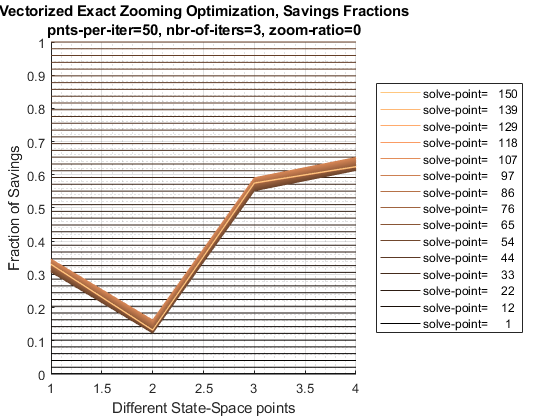
\includegraphics[width=5.20833in,height=\textheight]{img/fx_optim_mzoom_savezrone_images/figure_0.png}

\begin{verbatim}
    iter    cl_row_names_a      Var1         Var2        Var3         Var4  
    ____    ______________    _________    ________    _________    ________

     1        "point=1"         -3.6912     -1.9565       -12.83     -14.789
     1        "point=2"        0.058694    -0.80561      -2.4984     -2.1254
     1        "point=3"         0.38043    -0.72015      -1.5784    -0.99337
     1        "point=4"         0.55947    -0.67935      -1.0493    -0.34024
     1        "point=5"         0.67979    -0.65711     -0.68055     0.11647
     1        "point=6"          0.7677    -0.64529     -0.39997     0.46531
     1        "point=7"          0.8349    -0.64026     -0.17534     0.74571
     1        "point=8"         0.88763     -0.6401     0.010483      0.9787
     1        "point=9"         0.92959    -0.64367      0.16774      1.1768
     1        "point=10"        0.96316    -0.65026      0.30302      1.3481
     1        "point=11"        0.98996    -0.65938       0.4208      1.4981
     1        "point=12"         1.0111    -0.67071      0.52427      1.6308
     1        "point=13"         1.0275      -0.684      0.61578      1.7489
     1        "point=14"         1.0397     -0.6991      0.69709      1.8547
     1        "point=15"         1.0482    -0.71588      0.76958      1.9499
     1        "point=16"         1.0533    -0.73426      0.83429      2.0357
     1        "point=17"         1.0554    -0.75419       0.8921      2.1132
     1        "point=18"         1.0546    -0.77564      0.94367      2.1833
     1        "point=19"         1.0512    -0.79861      0.98955      2.2467
     1        "point=20"         1.0451    -0.82309       1.0302      2.3039
     1        "point=21"         1.0366     -0.8491        1.066      2.3554
     1        "point=22"         1.0256    -0.87669       1.0971      2.4015
     1        "point=23"         1.0123    -0.90591        1.124      2.4425
     1        "point=24"        0.99654    -0.93682       1.1466      2.4788
     1        "point=25"        0.97838     -0.9695       1.1652      2.5104
     1        "point=26"        0.95775      -1.004       1.1798      2.5375
     1        "point=27"        0.93459     -1.0406       1.1905      2.5602
     1        "point=28"        0.90881     -1.0792       1.1973      2.5785
     1        "point=29"        0.88029     -1.1202       1.2002      2.5925
     1        "point=30"        0.84886     -1.1635       1.1991      2.6022
     1        "point=31"        0.81434     -1.2096       1.1938      2.6073
     1        "point=32"        0.77649     -1.2587       1.1843      2.6078
     1        "point=33"        0.73504     -1.3109       1.1703      2.6035
     1        "point=34"        0.68964     -1.3668       1.1514       2.594
     1        "point=35"        0.63987     -1.4268       1.1274      2.5792
     1        "point=36"        0.58522     -1.4913       1.0978      2.5584
     1        "point=37"        0.52505     -1.5611        1.062      2.5312
     1        "point=38"        0.45857     -1.6369       1.0192      2.4968
     1        "point=39"        0.38475     -1.7198      0.96837      2.4541
     1        "point=40"         0.3023     -1.8111      0.90834      2.4021
     1        "point=41"        0.20947     -1.9126      0.83737      2.3388
     1        "point=42"        0.10391     -2.0266      0.75313      2.2622
     1        "point=43"      -0.017693     -2.1564      0.65234      2.1687
     1        "point=44"       -0.16019     -2.3069      0.53016      2.0538
     1        "point=45"       -0.33112     -2.4857      0.37908      1.9097
     1        "point=46"       -0.54312     -2.7054      0.18649       1.724
     1        "point=47"       -0.81989     -2.9896    -0.071303      1.4729
     1        "point=48"        -1.2146     -3.3917     -0.44748      1.1033
     1        "point=49"        -1.8971     -4.0814      -1.1118     0.44547
     1        "point=50"        -9.5085       -11.7      -8.7054     -7.1418
     2        "point=1"          1.0535    -0.64017       1.1975      2.6074
     2        "point=2"          1.0536    -0.64009       1.1977      2.6075
     2        "point=3"          1.0537    -0.64001       1.1979      2.6076
     2        "point=4"          1.0539    -0.63995        1.198      2.6077
     2        "point=5"           1.054    -0.63989       1.1982      2.6077
     2        "point=6"          1.0541    -0.63983       1.1984      2.6078
     2        "point=7"          1.0542    -0.63979       1.1985      2.6079
     2        "point=8"          1.0543    -0.63975       1.1986      2.6079
     2        "point=9"          1.0544    -0.63971       1.1988       2.608
     2        "point=10"         1.0545    -0.63969       1.1989       2.608
     2        "point=11"         1.0546    -0.63967        1.199      2.6081
     2        "point=12"         1.0547    -0.63966       1.1992      2.6081
     2        "point=13"         1.0548    -0.63965       1.1993      2.6081
     2        "point=14"         1.0548    -0.63965       1.1994      2.6081
     2        "point=15"         1.0549    -0.63966       1.1995      2.6081
     2        "point=16"          1.055    -0.63967       1.1996      2.6081
     2        "point=17"         1.0551    -0.63969       1.1997      2.6081
     2        "point=18"         1.0551    -0.63971       1.1998      2.6081
     2        "point=19"         1.0552    -0.63975       1.1998      2.6081
     2        "point=20"         1.0552    -0.63978       1.1999      2.6081
     2        "point=21"         1.0553    -0.63983          1.2       2.608
     2        "point=22"         1.0553    -0.63988          1.2       2.608
     2        "point=23"         1.0553    -0.63993       1.2001      2.6079
     2        "point=24"         1.0554    -0.63999       1.2001      2.6079
     2        "point=25"         1.0554    -0.64006       1.2002      2.6078
     2        "point=26"         1.0554    -0.64013       1.2002      2.6077
     2        "point=27"         1.0555    -0.64021       1.2002      2.6077
     2        "point=28"         1.0555    -0.64029       1.2003      2.6076
     2        "point=29"         1.0555    -0.64038       1.2003      2.6075
     2        "point=30"         1.0555    -0.64048       1.2003      2.6074
     2        "point=31"         1.0555    -0.64058       1.2003      2.6073
     2        "point=32"         1.0555    -0.64069       1.2003      2.6071
     2        "point=33"         1.0555     -0.6408       1.2003       2.607
     2        "point=34"         1.0555    -0.64091       1.2003      2.6069
     2        "point=35"         1.0555    -0.64104       1.2002      2.6067
     2        "point=36"         1.0554    -0.64116       1.2002      2.6066
     2        "point=37"         1.0554    -0.64129       1.2002      2.6064
     2        "point=38"         1.0554    -0.64143       1.2001      2.6063
     2        "point=39"         1.0554    -0.64157       1.2001      2.6061
     2        "point=40"         1.0553    -0.64172       1.2001      2.6059
     2        "point=41"         1.0553    -0.64188          1.2      2.6057
     2        "point=42"         1.0552    -0.64203       1.1999      2.6056
     2        "point=43"         1.0552     -0.6422       1.1999      2.6053
     2        "point=44"         1.0551    -0.64236       1.1998      2.6051
     2        "point=45"         1.0551    -0.64254       1.1997      2.6049
     2        "point=46"          1.055    -0.64271       1.1996      2.6047
     2        "point=47"         1.0549    -0.64289       1.1995      2.6045
     2        "point=48"         1.0549    -0.64308       1.1994      2.6042
     2        "point=49"         1.0548    -0.64327       1.1993       2.604
     2        "point=50"         1.0547    -0.64347       1.1992      2.6037
     3        "point=1"          1.0555    -0.63967       1.2003      2.6081
     3        "point=2"          1.0555    -0.63967       1.2003      2.6081
     3        "point=3"          1.0555    -0.63967       1.2003      2.6081
     3        "point=4"          1.0555    -0.63967       1.2003      2.6081
     3        "point=5"          1.0555    -0.63967       1.2003      2.6081
     3        "point=6"          1.0555    -0.63967       1.2003      2.6081
     3        "point=7"          1.0555    -0.63967       1.2003      2.6081
     3        "point=8"          1.0555    -0.63966       1.2003      2.6081
     3        "point=9"          1.0555    -0.63966       1.2003      2.6081
     3        "point=10"         1.0555    -0.63966       1.2003      2.6081
     3        "point=11"         1.0555    -0.63966       1.2003      2.6081
     3        "point=12"         1.0555    -0.63966       1.2003      2.6081
     3        "point=13"         1.0555    -0.63966       1.2003      2.6081
     3        "point=14"         1.0555    -0.63966       1.2003      2.6081
     3        "point=15"         1.0555    -0.63966       1.2003      2.6081
     3        "point=16"         1.0555    -0.63966       1.2003      2.6081
     3        "point=17"         1.0555    -0.63966       1.2003      2.6081
     3        "point=18"         1.0555    -0.63966       1.2003      2.6081
     3        "point=19"         1.0555    -0.63966       1.2003      2.6081
     3        "point=20"         1.0555    -0.63966       1.2003      2.6081
     3        "point=21"         1.0555    -0.63966       1.2003      2.6081
     3        "point=22"         1.0555    -0.63966       1.2003      2.6081
     3        "point=23"         1.0555    -0.63966       1.2003      2.6081
     3        "point=24"         1.0555    -0.63966       1.2003      2.6081
     3        "point=25"         1.0555    -0.63966       1.2003      2.6081
     3        "point=26"         1.0555    -0.63966       1.2003      2.6081
     3        "point=27"         1.0555    -0.63966       1.2003      2.6081
     3        "point=28"         1.0555    -0.63966       1.2003      2.6081
     3        "point=29"         1.0555    -0.63966       1.2003      2.6081
     3        "point=30"         1.0555    -0.63966       1.2003      2.6081
     3        "point=31"         1.0555    -0.63965       1.2003      2.6081
     3        "point=32"         1.0555    -0.63965       1.2003      2.6081
     3        "point=33"         1.0555    -0.63965       1.2003      2.6081
     3        "point=34"         1.0555    -0.63965       1.2003      2.6081
     3        "point=35"         1.0555    -0.63965       1.2003      2.6081
     3        "point=36"         1.0555    -0.63965       1.2003      2.6081
     3        "point=37"         1.0555    -0.63965       1.2003      2.6081
     3        "point=38"         1.0555    -0.63965       1.2003      2.6081
     3        "point=39"         1.0555    -0.63965       1.2003      2.6081
     3        "point=40"         1.0555    -0.63965       1.2003      2.6081
     3        "point=41"         1.0555    -0.63965       1.2003      2.6081
     3        "point=42"         1.0555    -0.63965       1.2003      2.6081
     3        "point=43"         1.0555    -0.63965       1.2003      2.6081
     3        "point=44"         1.0555    -0.63965       1.2003      2.6081
     3        "point=45"         1.0555    -0.63965       1.2003      2.6081
     3        "point=46"         1.0555    -0.63965       1.2003      2.6081
     3        "point=47"         1.0555    -0.63965       1.2003      2.6081
     3        "point=48"         1.0555    -0.63965       1.2003      2.6081
     3        "point=49"         1.0555    -0.63965       1.2003      2.6081
     3        "point=50"         1.0555    -0.63965       1.2003      2.6081
\end{verbatim}

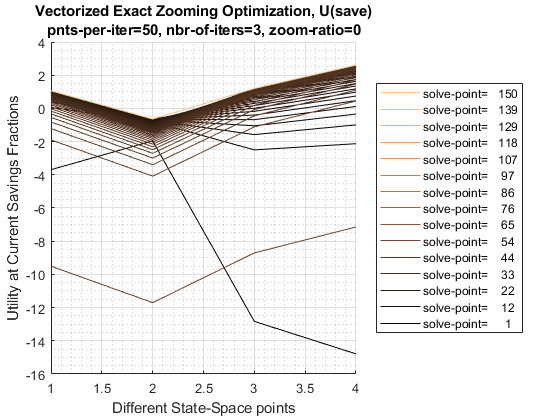
\includegraphics[width=5.20833in,height=\textheight]{img/fx_optim_mzoom_savezrone_images/figure_1.png}

\begin{verbatim}
Elapsed time is 1.292487 seconds.
----------------------------------------
xxxxxxxxxxxxxxxxxxxxxxxxxxxxxxxxxxxxxxxx
CONTAINER NAME: mp_container_map ND Array (Matrix etc)
xxxxxxxxxxxxxxxxxxxxxxxxxxxxxxxxxxxxxxxx
                         i    idx    ndim    numel    rowN    colN     sum       mean      std      coefvari      min         max  
                         _    ___    ____    _____    ____    ____    ______    ______    ______    ________    ________    _______

    ar_opti_foc_obj      1     1      2        4       1       4      4.2243    1.0561    1.3298     1.2592     -0.63965     2.6081
    ar_opti_save_frac    2     2      2        4       4       1       1.664     0.416    0.2284    0.54904      0.13278    0.62461

xxx TABLE:ar_opti_foc_obj xxxxxxxxxxxxxxxxxx
            c1         c2         c3        c4  
          ______    ________    ______    ______

    r1    1.0555    -0.63965    1.2003    2.6081

xxx TABLE:ar_opti_save_frac xxxxxxxxxxxxxxxxxx
            c1   
          _______

    r1    0.33086
    r2    0.13278
    r3    0.57575
    r4    0.62461
\end{verbatim}

\hypertarget{test-ff_optim_mzoom_savezrone-8-individuals-3-iterations-10-points-per-iteration-0.25-zoom-in-ratio}{%
\subsection{Test FF\_OPTIM\_MZOOM\_SAVEZRONE 8 Individuals 3 Iterations 10 Points Per Iteration, 0.25 zoom in ratio}\label{test-ff_optim_mzoom_savezrone-8-individuals-3-iterations-10-points-per-iteration-0.25-zoom-in-ratio}}

10 grid points per iteration, and 3 iterations.

\begin{verbatim}
% Generate the state-space and function
rng(123);
it_draws = 8; % must be even number
ar_z1 = exp(rand([it_draws,1])*3-1.5);
ar_z2 = exp(rand([it_draws,1])*3-1.5);
ar_r = (rand(it_draws,1)*10.0);
ar_beta = [rand(round(it_draws/2),1)*0.9+0.1; rand(round(it_draws/2),1)*0.9+1]; 
fc_util = @(x) ffi_intertemporal_util(x, ar_z1, ar_z2, ar_r, ar_beta);
% Call Function
bl_verbose = true;
bl_timer = true;
mp_mzoom_ctrlinfo = containers.Map('KeyType','char', 'ValueType','any');
mp_mzoom_ctrlinfo('it_mzoom_jnt_pnts') = 10;
mp_mzoom_ctrlinfo('it_mzoom_max_iter') = 3;
mp_mzoom_ctrlinfo('it_mzoom_zm_ratio') = 0.25;
ff_optim_mzoom_savezrone(fc_util, bl_verbose, bl_timer, mp_mzoom_ctrlinfo);

    iter    cl_row_names_a     Var1       Var2       Var3       Var4       Var5       Var6       Var7       Var8  
    ____    ______________    _______    _______    _______    _______    _______    _______    _______    _______

     1        "point=1"         1e-05      1e-05      1e-05      1e-05      1e-05      1e-05      1e-05      1e-05
     1        "point=2"       0.11112    0.11112    0.11112    0.11112    0.11112    0.11112    0.11112    0.11112
     1        "point=3"       0.22223    0.22223    0.22223    0.22223    0.22223    0.22223    0.22223    0.22223
     1        "point=4"       0.33334    0.33334    0.33334    0.33334    0.33334    0.33334    0.33334    0.33334
     1        "point=5"       0.44445    0.44445    0.44445    0.44445    0.44445    0.44445    0.44445    0.44445
     1        "point=6"       0.55555    0.55555    0.55555    0.55555    0.55555    0.55555    0.55555    0.55555
     1        "point=7"       0.66666    0.66666    0.66666    0.66666    0.66666    0.66666    0.66666    0.66666
     1        "point=8"       0.77777    0.77777    0.77777    0.77777    0.77777    0.77777    0.77777    0.77777
     1        "point=9"       0.88888    0.88888    0.88888    0.88888    0.88888    0.88888    0.88888    0.88888
     1        "point=10"      0.99999    0.99999    0.99999    0.99999    0.99999    0.99999    0.99999    0.99999
     2        "point=1"       0.28788    0.20455    0.20455    0.12122    0.37121    0.37121    0.37121    0.37121
     2        "point=2"       0.32576    0.24243    0.24243     0.1591    0.40909    0.40909    0.40909    0.40909
     2        "point=3"       0.36364    0.28031    0.28031    0.19698    0.44697    0.44697    0.44697    0.44697
     2        "point=4"       0.40152    0.31819    0.31819    0.23485    0.48485    0.48485    0.48485    0.48485
     2        "point=5"        0.4394    0.35606    0.35606    0.27273    0.52273    0.52273    0.52273    0.52273
     2        "point=6"       0.47727    0.39394    0.39394    0.31061     0.5606     0.5606     0.5606     0.5606
     2        "point=7"       0.51515    0.43182    0.43182    0.34849    0.59848    0.59848    0.59848    0.59848
     2        "point=8"       0.55303     0.4697     0.4697    0.38637    0.63636    0.63636    0.63636    0.63636
     2        "point=9"       0.59091    0.50758    0.50758    0.42424    0.67424    0.67424    0.67424    0.67424
     2        "point=10"      0.62879    0.54545    0.54545    0.46212    0.71212    0.71212    0.71212    0.71212
     3        "point=1"       0.34987    0.20972    0.20972    0.15479    0.46161    0.49001     0.4332    0.49001
     3        "point=2"        0.3645    0.22435    0.22435    0.16943    0.47624    0.50465    0.44783    0.50465
     3        "point=3"       0.37913    0.23899    0.23899    0.18406    0.49087    0.51928    0.46247    0.51928
     3        "point=4"       0.39377    0.25362    0.25362     0.1987    0.50551    0.53392     0.4771    0.53392
     3        "point=5"        0.4084    0.26826    0.26826    0.21333    0.52014    0.54855    0.49174    0.54855
     3        "point=6"       0.42304    0.28289    0.28289    0.22797    0.53478    0.56319    0.50637    0.56319
     3        "point=7"       0.43767    0.29752    0.29752     0.2426    0.54941    0.57782    0.52101    0.57782
     3        "point=8"       0.45231    0.31216    0.31216    0.25724    0.56405    0.59246    0.53564    0.59246
     3        "point=9"       0.46694    0.32679    0.32679    0.27187    0.57868    0.60709    0.55027    0.60709
     3        "point=10"      0.48158    0.34143    0.34143    0.28651    0.59332    0.62173    0.56491    0.62173
\end{verbatim}

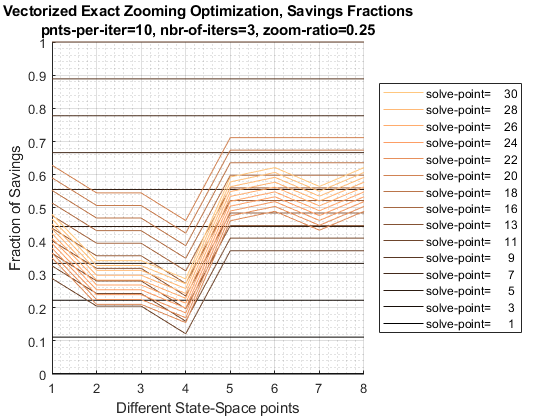
\includegraphics[width=5.20833in,height=\textheight]{img/fx_optim_mzoom_savezrone_images/figure_2.png}

\begin{verbatim}
    iter    cl_row_names_a      Var1        Var2        Var3        Var4       Var5        Var6       Var7       Var8  
    ____    ______________    ________    ________    ________    ________    _______    ________    _______    _______

     1        "point=1"        -6.5286     -4.4312     -4.9951     -2.4407    -10.415     -15.025    -7.1352    -11.589
     1        "point=2"        0.34227    -0.90966      -1.148     0.28691     1.2451    -0.53687      2.835      1.245
     1        "point=3"         0.7287    -0.77242    -0.98657     0.36508     1.9879      0.4163      3.452     2.0751
     1        "point=4"        0.87872    -0.76818    -0.96816     0.33477     2.3463     0.89785      3.737     2.4847
     1        "point=5"        0.91222    -0.83811      -1.028     0.24031     2.5277      1.1666     3.8662     2.7023
     1        "point=6"        0.85648    -0.97408     -1.1562    0.085331     2.5867      1.2933     3.8847     2.7894
     1        "point=7"        0.70558     -1.1905     -1.3663    -0.14666     2.5296      1.2915     3.7944     2.7552
     1        "point=8"        0.41577     -1.5358     -1.7061    -0.50502      2.319      1.1277     3.5559     2.5641
     1        "point=9"       -0.17716     -2.1767     -2.3424     -1.1573     1.7947     0.64395     3.0074     2.0566
     1        "point=10"       -9.4046     -11.446     -11.608     -10.437    -7.3721     -8.4872    -6.1808    -7.0954
     2        "point=1"         0.8347    -0.78233    -0.99938     0.30205     2.4239      1.0081      3.795     2.5758
     2        "point=2"        0.87277    -0.76475    -0.97586     0.34105     2.4846      1.0983     3.8381     2.6488
     2        "point=3"        0.89748    -0.75933    -0.96536     0.36018     2.5303      1.1709     3.8677     2.7056
     2        "point=4"        0.91044    -0.76388    -0.96549     0.36559     2.5622      1.2275     3.8849     2.7478
     2        "point=5"        0.91269     -0.7771    -0.97477     0.36049      2.581       1.269       3.89      2.776
     2        "point=6"        0.90477    -0.79823    -0.99237     0.34672     2.5867       1.296      3.883     2.7906
     2        "point=7"        0.88684     -0.8269     -1.0178     0.32535     2.5793      1.3084     3.8637     2.7913
     2        "point=8"        0.85872    -0.86304      -1.051     0.29697     2.5578      1.3055      3.831     2.7776
     2        "point=9"        0.81987    -0.90685     -1.0921     0.26182     2.5209      1.2862     3.7837      2.748
     2        "point=10"       0.76932    -0.95877     -1.1415     0.21989     2.4664      1.2483     3.7192     2.7003
     3        "point=1"        0.88992     -0.7791    -0.99528     0.33777     2.5443       1.234     3.8584     2.7524
     3        "point=2"         0.8979    -0.77144    -0.98526      0.3479     2.5562       1.251     3.8683     2.7642
     3        "point=3"        0.90413     -0.7658    -0.97741     0.35543     2.5661      1.2659     3.8762      2.774
     3        "point=4"        0.90869      -0.762    -0.97154      0.3607     2.5741      1.2785     3.8824     2.7817
     3        "point=5"        0.91163    -0.75989    -0.96746     0.36397     2.5801       1.289     3.8867     2.7874
     3        "point=6"        0.91299    -0.75934    -0.96506     0.36546     2.5842      1.2974     3.8892     2.7911
     3        "point=7"        0.91281    -0.76025    -0.96421     0.36532     2.5864      1.3035       3.89     2.7927
     3        "point=8"        0.91112    -0.76255    -0.96482      0.3637     2.5866      1.3074      3.889     2.7922
     3        "point=9"        0.90792    -0.76615    -0.96683      0.3607     2.5849      1.3091     3.8861     2.7895
     3        "point=10"       0.90324    -0.77102    -0.97016     0.35641     2.5811      1.3085     3.8815     2.7847
\end{verbatim}

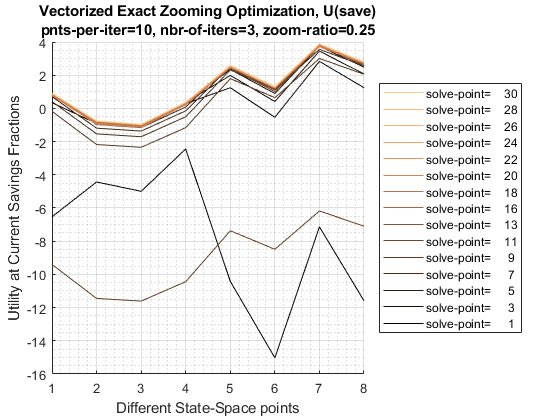
\includegraphics[width=5.20833in,height=\textheight]{img/fx_optim_mzoom_savezrone_images/figure_3.png}

\begin{verbatim}
Elapsed time is 1.047404 seconds.
----------------------------------------
xxxxxxxxxxxxxxxxxxxxxxxxxxxxxxxxxxxxxxxx
CONTAINER NAME: mp_container_map ND Array (Matrix etc)
xxxxxxxxxxxxxxxxxxxxxxxxxxxxxxxxxxxxxxxx
                         i    idx    ndim    numel    rowN    colN     sum       mean        std      coefvari      min         max  
                         _    ___    ____    _____    ____    ____    ______    _______    _______    ________    ________    _______

    ar_opti_foc_obj      1     1      2        8       1       8      10.125     1.2656      1.731     1.3677     -0.96506     3.8892
    ar_opti_save_frac    2     2      2        8       8       1      3.3843    0.42304    0.15074    0.35632      0.21333    0.59246

xxx TABLE:ar_opti_foc_obj xxxxxxxxxxxxxxxxxx
            c1          c2          c3         c4         c5        c6        c7        c8  
          _______    ________    ________    _______    ______    ______    ______    ______

    r1    0.91163    -0.75989    -0.96506    0.36397    2.5864    1.3074    3.8892    2.7911

xxx TABLE:ar_opti_save_frac xxxxxxxxxxxxxxxxxx
            c1   
          _______

    r1     0.4084
    r2    0.26826
    r3    0.28289
    r4    0.21333
    r5    0.54941
    r6    0.59246
    r7    0.50637
    r8    0.56319
\end{verbatim}

\hypertarget{test-ff_optim_mzoom_savezrone-speed}{%
\subsection{Test FF\_OPTIM\_MZOOM\_SAVEZRONE Speed}\label{test-ff_optim_mzoom_savezrone-speed}}

Test Speed doing 6.25 million state-spcae points for a savings problem:

\begin{verbatim}
% Generate the state-space and function
rng(123);
it_draws = 6250000; % must be even number
ar_z1 = exp(rand([it_draws,1])*3-1.5);
ar_z2 = exp(rand([it_draws,1])*3-1.5);
ar_r = (rand(it_draws,1)*10.0);
ar_beta = [rand(round(it_draws/2),1)*0.9+0.1; rand(round(it_draws/2),1)*0.9+1]; 
% ffi_intertemporal_max is a function in ff_optim_mlsec_savezrone for testing
fc_util = @(x) ffi_intertemporal_util(x, ar_z1, ar_z2, ar_r, ar_beta);
% Call Function
bl_verbose = false;
bl_timer = true;
% set parameters
mp_mzoom_ctrlinfo = containers.Map('KeyType','char', 'ValueType','any');
mp_mzoom_ctrlinfo('it_mzoom_jnt_pnts') = 20;
mp_mzoom_ctrlinfo('it_mzoom_max_iter') = 10;
mp_mzoom_ctrlinfo('it_mzoom_zm_ratio') = 0.25;
[ar_opti_save_frac, ar_opti_save_level] = ...
    ff_optim_mzoom_savezrone(fc_util, bl_verbose, bl_timer, mp_mzoom_ctrlinfo);

Elapsed time is 54.241104 seconds.

mp_container_map = containers.Map('KeyType','char', 'ValueType','any');
mp_container_map('ar_opti_save_frac') = ar_opti_save_frac;
mp_container_map('ar_opti_save_level') = ar_opti_save_level;
mp_container_map('ar_opti_save_frac_notnan') = ar_opti_save_frac(~isnan(ar_opti_save_frac));
ff_container_map_display(mp_container_map);

----------------------------------------
xxxxxxxxxxxxxxxxxxxxxxxxxxxxxxxxxxxxxxxx
CONTAINER NAME: mp_container_map ND Array (Matrix etc)
xxxxxxxxxxxxxxxxxxxxxxxxxxxxxxxxxxxxxxxx
                                i    idx    ndim     numel        rowN      colN       sum         mean        std      coefvari      min         max  
                                _    ___    ____    ________    ________    ____    __________    _______    _______    ________    ________    _______

    ar_opti_save_frac           1     1      2      6.25e+06    6.25e+06     1      2.8839e+06    0.46142    0.15305     0.3317     0.090907    0.65513
    ar_opti_save_frac_notnan    2     2      2      6.25e+06    6.25e+06     1      2.8839e+06    0.46142    0.15305     0.3317     0.090907    0.65513
    ar_opti_save_level          3     3      2      6.25e+06    6.25e+06     1      2.9481e+06    0.47169    0.66665     1.4133      -3.9806     2.9221

figure();
histogram(ar_opti_save_frac(~isnan(ar_opti_save_frac)),100);
title('Distribution of Optimal Savings Fractions');
xlabel('Savings Fractions');
grid on;
\end{verbatim}

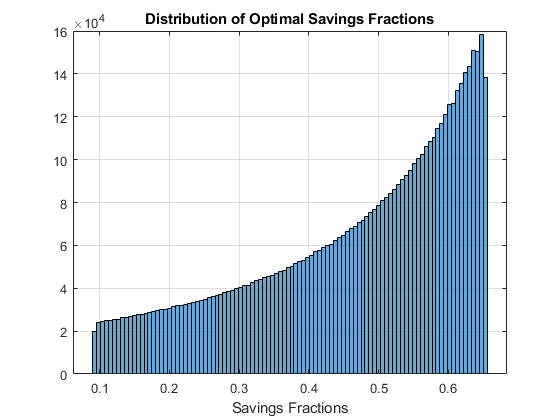
\includegraphics[width=5.20833in,height=\textheight]{img/fx_optim_mzoom_savezrone_images/figure_4.png}

\hypertarget{define-two-period-intertemporal-log-utility-no-shock-utility-function}{%
\subsection{Define Two Period Intertemporal Log Utility No Shock Utility Function}\label{define-two-period-intertemporal-log-utility-no-shock-utility-function}}

See \href{https://fanwangecon.github.io/Math4Econ/derivative_application/htmlpdfm/K_save_households.html}{Household's Utility Maximization Problem and Two-Period Borrowing
and Savings Problem given
Endowments}.

\begin{verbatim}
function [ar_util, ar_saveborr_level] = ...
    ffi_intertemporal_util(ar_saveborr_frac, z1, z2, r, beta)

ar_saveborr_level = ar_saveborr_frac.*(z1+z2./(1+r)) - z2./(1+r);
ar_util = log(z1 - ar_saveborr_level) + beta.*log(ar_saveborr_level.*(1+r) + z2);

end
\end{verbatim}

\hypertarget{graphs}{%
\chapter{Graphs}\label{graphs}}

\hypertarget{ff_graph_grid-examples-x-y-and-color-line-plots}{%
\section{FF\_GRAPH\_GRID Examples: X, Y and Color Line Plots}\label{ff_graph_grid-examples-x-y-and-color-line-plots}}

\begin{quote}
Go back to \href{http://fanwangecon.github.io/}{fan}'s \href{https://fanwangecon.github.io/MEconTools/}{MEconTools} Toolbox (\href{https://fanwangecon.github.io/MEconTools/bookdown}{bookdown}), \href{https://fanwangecon.github.io/M4Econ/}{Matlab Code Examples} Repository (\href{https://fanwangecon.github.io/M4Econ/bookdown}{bookdown}), or \href{https://fanwangecon.github.io/Math4Econ/}{Math for Econ with Matlab} Repository (\href{https://fanwangecon.github.io/Math4Econ/bookdown}{bookdown}).
\end{quote}

This is the example vignette for function:
\href{https://github.com/FanWangEcon/MEconTools/blob/master/MEconTools/graph/ff_graph_grid.m}{\textbf{ff\_graph\_grid}}
from the \href{https://fanwangecon.github.io/MEconTools/}{\textbf{MEconTools
Package}}\textbf{.} This function
can graph out value and policy functions given one state vector
(x-axis), conditional on other states (line groups). Can handle a few
lines (scatter + lines), or many groups (jet spectrum).

\hypertarget{test-ff_graph_grid-defaults}{%
\subsection{Test FF\_GRAPH\_GRID Defaults}\label{test-ff_graph_grid-defaults}}

Call the function with defaults.

\begin{verbatim}
ff_graph_grid();
\end{verbatim}

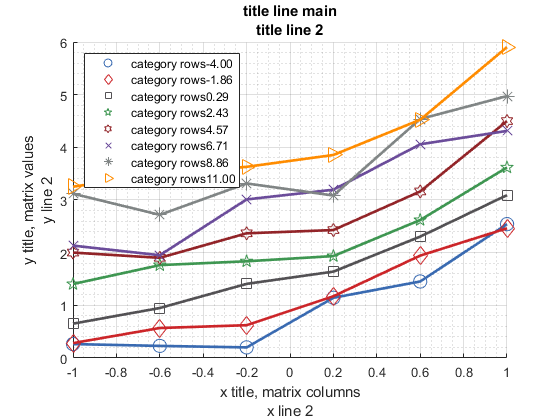
\includegraphics[width=5.20833in,height=\textheight]{img/fx_graph_grid_images/figure_0.png}

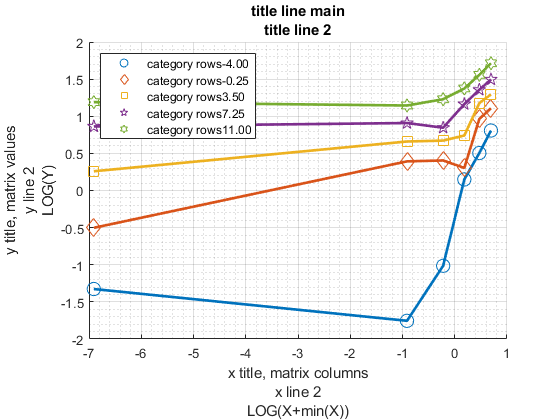
\includegraphics[width=5.20833in,height=\textheight]{img/fx_graph_grid_images/figure_1.png}

\hypertarget{test-ff_graph_grid-random-matrix-pick-markers-and-colors}{%
\subsection{Test FF\_GRAPH\_GRID Random Matrix Pick Markers and Colors}\label{test-ff_graph_grid-random-matrix-pick-markers-and-colors}}

Call the function with defaults.

\begin{verbatim}
rng(123);
mt_value = [normrnd(50,10,[1, 50]); ...
            normrnd(70,5,[1, 50]);...
            normrnd(90,10,[1, 50])];
ar_row_grid = ["shock low", "zero", "shock high"];
ar_col_grid = 1:50;
mp_support_graph = containers.Map('KeyType', 'char', 'ValueType', 'any');
mp_support_graph('cl_scatter_shapes') = { '.', 's' ,'.' };
mp_support_graph('cl_colors') = {'gray', 'red', 'gray'};
ff_graph_grid(mt_value, ar_row_grid, ar_col_grid, mp_support_graph);
\end{verbatim}

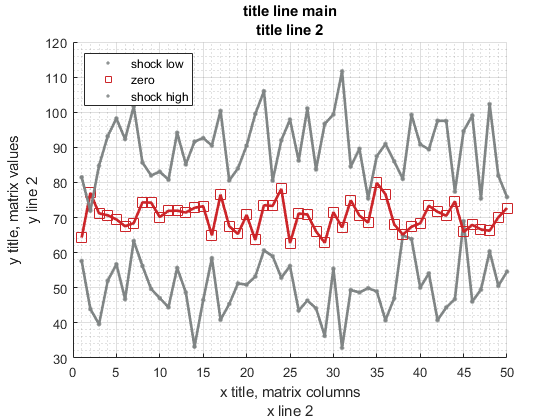
\includegraphics[width=5.20833in,height=\textheight]{img/fx_graph_grid_images/figure_2.png}

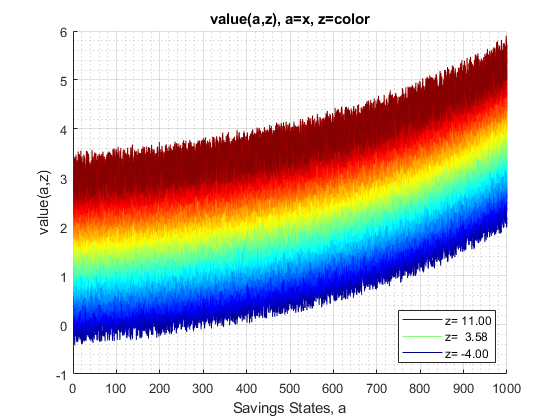
\includegraphics[width=5.20833in,height=\textheight]{img/fx_graph_grid_images/figure_3.png}

\hypertarget{test-ff_graph_grid-two-random-normal-lines-and-labels}{%
\subsection{Test FF\_GRAPH\_GRID Two Random Normal Lines and Labels}\label{test-ff_graph_grid-two-random-normal-lines-and-labels}}

There are two autoregressive time series, plot out the time two time
series.

\begin{verbatim}
% Generate the two time series
rng(456);
mt_value = normrnd(100,10,[2, 50]);
ar_row_grid = ["individual 1", "individual 2"];
ar_col_grid = 1:50;
mp_support_graph = containers.Map('KeyType', 'char', 'ValueType', 'any');
mp_support_graph('cl_st_graph_title') = {'Time Series Two Individuals'};
mp_support_graph('cl_st_ytitle') = {'Values'};
mp_support_graph('cl_st_xtitle') = {'Periods'};
mp_support_graph('bl_graph_logy') = false; % do not log
ff_graph_grid(mt_value, ar_row_grid, ar_col_grid, mp_support_graph);
\end{verbatim}

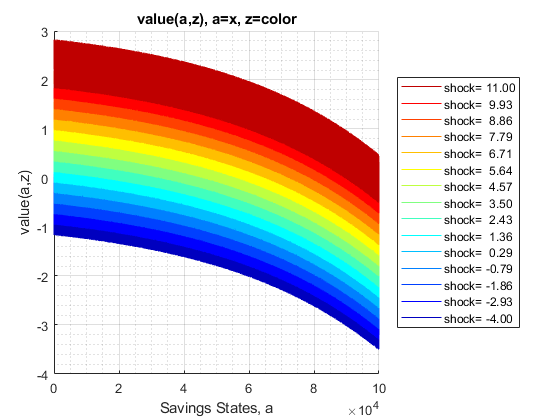
\includegraphics[width=5.20833in,height=\textheight]{img/fx_graph_grid_images/figure_4.png}

\hypertarget{test-ff_graph_grid-6-lines-pick-marker-and-colors}{%
\subsection{Test FF\_GRAPH\_GRID 6 Lines Pick Marker and Colors}\label{test-ff_graph_grid-6-lines-pick-marker-and-colors}}

Plot many lines, with auto legend.

\begin{verbatim}
% Generate some Data
rng(456);
ar_row_grid = linspace(-4, 11, 5);
ar_col_grid = linspace(-1, 1, 20);
rng(123);
mt_value = 0.2*ar_row_grid' + exp(ar_col_grid) + rand([length(ar_row_grid), length(ar_col_grid)]);
% container map settings
mp_support_graph = containers.Map('KeyType', 'char', 'ValueType', 'any');
mp_support_graph('cl_st_graph_title') = {'5 lines, specify marker and color, value(a,z), a=x, z=color'};
mp_support_graph('cl_st_ytitle') = {'value(a,z)'};
mp_support_graph('cl_st_xtitle') = {'Savings States, a'};
mp_support_graph('st_legend_loc') = 'southeast';
mp_support_graph('bl_graph_logy') = false; % do not log
mp_support_graph('st_rowvar_name') = 'z=';
mp_support_graph('it_legend_select') = 3; % how many shock legends to show
mp_support_graph('st_rounding') = '6.2f'; % format shock legend
mp_support_graph('cl_scatter_shapes') = {'s', 's', '*', '*', 'p'};
mp_support_graph('cl_colors') = {'green', 'black', 'green', 'black', 'orange'};
% Call function
ff_graph_grid(mt_value, ar_row_grid, ar_col_grid, mp_support_graph);
\end{verbatim}

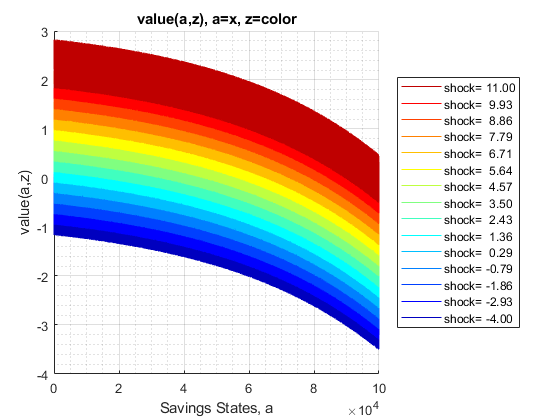
\includegraphics[width=5.20833in,height=\textheight]{img/fx_graph_grid_images/figure_5.png}

\hypertarget{test-ff_graph_grid-many-lines}{%
\subsection{Test FF\_GRAPH\_GRID Many Lines}\label{test-ff_graph_grid-many-lines}}

Plot many lines, with auto legend.

\begin{verbatim}
% Generate some Data
rng(456);
ar_row_grid = linspace(-4, 11, 100);
ar_col_grid = linspace(-1, 1, 1000);
rng(123);
mt_value = 0.2*ar_row_grid' + exp(ar_col_grid) + rand([length(ar_row_grid), length(ar_col_grid)]);
% container map settings
mp_support_graph = containers.Map('KeyType', 'char', 'ValueType', 'any');
mp_support_graph('cl_st_graph_title') = {'value(a,z), a=x, z=color'};
mp_support_graph('cl_st_ytitle') = {'value(a,z)'};
mp_support_graph('cl_st_xtitle') = {'Savings States, a'};
mp_support_graph('st_legend_loc') = 'southeast';
mp_support_graph('bl_graph_logy') = false; % do not log
mp_support_graph('st_rowvar_name') = 'z=';
mp_support_graph('it_legend_select') = 3; % how many shock legends to show
mp_support_graph('st_rounding') = '6.2f'; % format shock legend
mp_support_graph('cl_colors') = 'jet'; % any predefined matlab colormap
% Call function
ff_graph_grid(mt_value, ar_row_grid, ar_col_grid, mp_support_graph);
\end{verbatim}

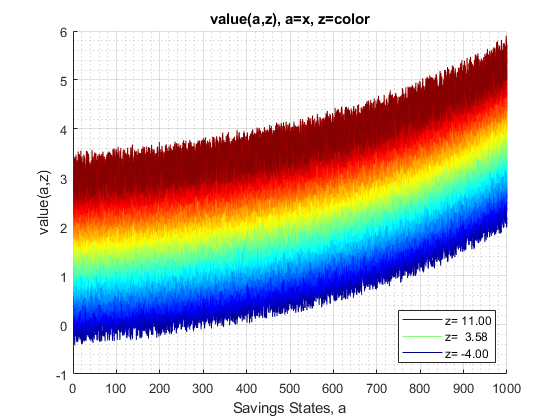
\includegraphics[width=5.20833in,height=\textheight]{img/fx_graph_grid_images/figure_6.png}

\hypertarget{test-ff_graph_grid-many-lines-legend-exogenous}{%
\subsection{Test FF\_GRAPH\_GRID Many Lines Legend Exogenous}\label{test-ff_graph_grid-many-lines-legend-exogenous}}

Plot many lines, exogenously set legend

\begin{verbatim}
% Generate the two time series
rng(456);
ar_row_grid = linspace(-4, 11, 15);
ar_col_grid = linspace(-1, 1, 100000);
rng(123);
mt_value = 0.2*ar_row_grid' - exp(ar_col_grid) + rand([length(ar_row_grid), length(ar_col_grid)]);
% setting shock vector name exogenously here
ar_row_grid = string(num2str(ar_row_grid', "shock=%6.2f"));
% container map settings
mp_support_graph = containers.Map('KeyType', 'char', 'ValueType', 'any');
mp_support_graph('cl_st_graph_title') = {'value(a,z), a=x, z=color'};
mp_support_graph('cl_st_ytitle') = {'value(a,z)'};
mp_support_graph('cl_st_xtitle') = {'Savings States, a'};
mp_support_graph('st_legend_loc') = 'eastoutside';
mp_support_graph('bl_graph_logy') = false; % do not log
mp_support_graph('it_legend_select') = 15;
mp_support_graph('cl_colors') = 'winter'; % any predefined matlab colormap
% Call function
ff_graph_grid(mt_value, ar_row_grid, ar_col_grid, mp_support_graph);
\end{verbatim}

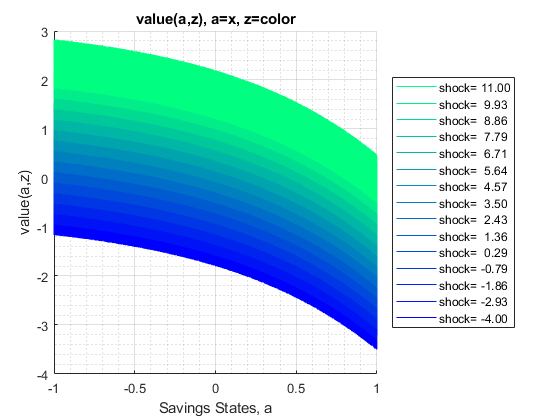
\includegraphics[width=5.20833in,height=\textheight]{img/fx_graph_grid_images/figure_7.png}

\hypertarget{support-tools}{%
\chapter{Support Tools}\label{support-tools}}

\hypertarget{ff_container_map_display-examples}{%
\section{FF\_CONTAINER\_MAP\_DISPLAY Examples}\label{ff_container_map_display-examples}}

\begin{quote}
Go back to \href{http://fanwangecon.github.io/}{fan}'s \href{https://fanwangecon.github.io/MEconTools/}{MEconTools} Toolbox (\href{https://fanwangecon.github.io/MEconTools/bookdown}{bookdown}), \href{https://fanwangecon.github.io/M4Econ/}{Matlab Code Examples} Repository (\href{https://fanwangecon.github.io/M4Econ/bookdown}{bookdown}), or \href{https://fanwangecon.github.io/Math4Econ/}{Math for Econ with Matlab} Repository (\href{https://fanwangecon.github.io/Math4Econ/bookdown}{bookdown}).
\end{quote}

This is the example vignette for function:
\href{https://github.com/FanWangEcon/MEconTools/blob/master/MEconTools/tools/ff_container_map_display.m}{\textbf{ff\_container\_map\_display}}
from the \href{https://fanwangecon.github.io/MEconTools/}{\textbf{MEconTools
Package}}\textbf{.} This function
summarizes statistics of matrixes stored in a container map, as well as
scalar, string, function and other values stored in container maps.

\hypertarget{test-ff_container_map_display-defaults}{%
\subsection{Test FF\_CONTAINER\_MAP\_DISPLAY Defaults}\label{test-ff_container_map_display-defaults}}

Call the function with defaults.

\begin{verbatim}
ff_container_map_display();

----------------------------------------
xxxxxxxxxxxxxxxxxxxxxxxxxxxxxxxxxxxxxxxx
 ND Array (Matrix etc)
xxxxxxxxxxxxxxxxxxxxxxxxxxxxxxxxxxxxxxxx
                      i     idx    ndim    numel    rowN    colN     sum       mean        std      coefvari       min          max  
                      __    ___    ____    _____    ____    ____    ______    _______    _______    ________    __________    _______

    mat_1              1     7      2        12       3       4     6.5142    0.54285     0.2232    0.41115        0.22685    0.98076
    mat_2              2     8      2      2650      50      53     1313.3    0.49559    0.29232    0.58985     6.7838e-05    0.99964
    mat_2_boolean      3     9      2      2650      50      53       1361    0.51358    0.49991    0.97337              0          1
    mat_3              4    10      2         4       2       2     1.8111    0.45277    0.45111    0.99635     0.00012471    0.88615
    tensor_1           5    15      3        16       2       8     7.3043    0.45652    0.27787    0.60867       0.018091     0.8345
    tensor_2           6    16      3        75       3      25     40.195    0.53593    0.29044    0.54194      0.0024293    0.99731
    tensor_3           7    17      2         4       1       4     1.6926    0.42315    0.37389    0.88359         0.1219    0.91553
    tesseract_1        8    18      4        72       3      24     34.321    0.47669    0.26374    0.55327       0.010239    0.96435
    tesseract_2        9    19      4        20       2      10     8.4191    0.42096    0.28981    0.68846       0.043114    0.97146
    tesseract_bl_3    10    20      4        10       1      10          3        0.3    0.48305     1.6102              0          1

xxx TABLE:mat_1 xxxxxxxxxxxxxxxxxx
            c1         c2         c3         c4   
          _______    _______    _______    _______

    r1    0.69647    0.55131    0.98076    0.39212
    r2    0.28614    0.71947    0.68483    0.34318
    r3    0.22685    0.42311    0.48093    0.72905

xxx TABLE:mat_2 xxxxxxxxxxxxxxxxxx
              c1          c2         c3          c4         c50         c51         c52         c53   
           ________    ________    _______    ________    ________    ________    ________    ________

    r1      0.43857      0.6249    0.17108     0.56564    0.072152     0.67855     0.61667     0.54002
    r2     0.059678     0.67469    0.82911    0.084904     0.63289     0.27236     0.32528     0.24957
    r3      0.39804     0.84234    0.33867     0.58267    0.046367     0.44513    0.075047      0.7839
    r4        0.738    0.083195    0.55237     0.81484     0.50561     0.11117     0.59532     0.35603
    r5      0.18249     0.76368    0.57855     0.33707     0.10653    0.028681      0.7435     0.91869
    r46      0.6813     0.55326    0.88786     0.69983     0.83758     0.16382     0.74191    0.065638
    r47     0.87546     0.85445    0.69631     0.66117     0.97069     0.79092     0.42466     0.78725
    r48     0.51042     0.38484    0.44033    0.049097    0.017768     0.33302     0.24401     0.97956
    r49     0.66931     0.31679    0.43821      0.7923     0.12979     0.75311     0.79466    0.079086
    r50     0.58594     0.35426     0.7651     0.51872     0.86415     0.58281     0.84795      0.4579

xxx TABLE:mat_2_boolean xxxxxxxxxxxxxxxxxx
            c1       c2       c3       c4       c50      c51      c52      c53 
           _____    _____    _____    _____    _____    _____    _____    _____

    r1     true     false    false    true     true     false    true     true 
    r2     true     false    true     true     false    false    true     true 
    r3     false    true     false    true     false    true     false    true 
    r4     false    true     false    false    false    true     true     true 
    r5     true     true     true     false    true     false    false    true 
    r46    false    true     true     false    true     true     true     true 
    r47    true     true     true     true     true     true     false    false
    r48    true     false    false    false    true     true     false    true 
    r49    true     true     false    true     true     true     false    false
    r50    false    false    false    false    false    false    false    false

xxx TABLE:mat_3 xxxxxxxxxxxxxxxxxx
              c1          c2   
          __________    _______

    r1    0.00012471    0.13253
    r2       0.88615    0.79226

xxx TABLE:tensor_1 xxxxxxxxxxxxxxxxxx
             c1         c2         c3         c4         c5         c6         c7        c8   
          ________    _______    _______    _______    _______    _______    ______    _______

    r1    0.019363    0.34271    0.52167    0.53703    0.75756    0.68839    0.8345    0.26597
    r2    0.018091    0.33355    0.11738    0.77857    0.81933    0.28644    0.6157      0.368

xxx TABLE:tensor_2 xxxxxxxxxxxxxxxxxx
             c1         c2         c3         c4         c22        c23         c24         c25  
          ________    _______    _______    _______    _______    _______    _________    _______

    r1     0.51866    0.40495    0.48278    0.99731    0.46584    0.62976     0.035924    0.10505
    r2    0.028692    0.37408    0.24149    0.35201    0.66054    0.87243    0.0024293    0.81088
    r3     0.87339    0.19457    0.83212    0.15315    0.77859    0.96663       0.2501     0.8056

xxx TABLE:tensor_3 xxxxxxxxxxxxxxxxxx
            c1        c2        c3         c4   
          ______    ______    _______    _______

    r1    0.1219    0.5119    0.91553    0.14329

xxx TABLE:tesseract_1 xxxxxxxxxxxxxxxxxx
            c1         c2         c3          c4         c21        c22        c23        c24  
          _______    _______    _______    ________    _______    _______    _______    _______

    r1    0.64531    0.59299    0.32115     0.67653    0.90328    0.56911    0.52562    0.12014
    r2    0.74558     0.5007    0.46142     0.21384    0.35564    0.13732      0.155    0.23786
    r3    0.91137    0.46403    0.18118    0.049919    0.46246    0.46842    0.75348    0.64547

xxx TABLE:tesseract_2 xxxxxxxxxxxxxxxxxx
             c1         c2         c3         c4         c7         c8          c9         c10  
          ________    _______    _______    _______    _______    _______    ________    _______

    r1     0.28898    0.48211    0.44359    0.97146    0.61782    0.65121     0.80715    0.11605
    r2    0.094493    0.34941    0.17595    0.14192    0.16754    0.57097    0.043114    0.70518

xxx TABLE:tesseract_bl_3 xxxxxxxxxxxxxxxxxx
           c1       c2       c3       c4       c7       c8       c9       c10 
          _____    _____    _____    _____    _____    _____    _____    _____

    r1    false    false    true     true     false    true     false    false

----------------------------------------
xxxxxxxxxxxxxxxxxxxxxxxxxxxxxxxxxxxxxxxx
 Scalars
xxxxxxxxxxxxxxxxxxxxxxxxxxxxxxxxxxxxxxxx
                      i    idx     value 
                      _    ___    _______

    boolean_1         1     1           1
    empty             2     2         NaN
    mat_4             3    11     0.74898
    string_float_1    4    13      1021.1
    string_int_1      5    14        1021

----------------------------------------
xxxxxxxxxxxxxxxxxxxxxxxxxxxxxxxxxxxxxxxx
 String
xxxxxxxxxxxxxxxxxxxxxxxxxxxxxxxxxxxxxxxx
                      i     idx            string        
                     ___    ____    _____________________

    list_string_1    "1"    "5"     "col1;col2;col3;col4"
    list_string_2    "2"    "6"     "row1;row2;row3;row4"
    string_1         "3"    "12"    "Table Name"         

----------------------------------------
xxxxxxxxxxxxxxxxxxxxxxxxxxxxxxxxxxxxxxxx
 Functions
xxxxxxxxxxxxxxxxxxxxxxxxxxxxxxxxxxxxxxxx
              i     idx      functionString   
             ___    ___    ___________________

    func1    "1"    "3"    "@(x)1+2+x"        
    func2    "2"    "4"    "@(x,y)x*1+sqrt(y)"
\end{verbatim}

\hypertarget{test-ff_container_map_display-summarize-matrix-only}{%
\subsection{Test FF\_CONTAINER\_MAP\_DISPLAY summarize Matrix Only}\label{test-ff_container_map_display-summarize-matrix-only}}

Three large matrixes, show summaries

\begin{verbatim}
% Create Container
mp_container_map = containers.Map('KeyType','char', 'ValueType','any');
rng(123);
mp_container_map('mat_1') = rand(100,100);
mp_container_map('mat_2') = rand(100,100)*2 + 1;
mp_container_map('mat_2_boolean') = (rand(100,100) > 0.5);
% Will only print 
ff_container_map_display(mp_container_map);

----------------------------------------
xxxxxxxxxxxxxxxxxxxxxxxxxxxxxxxxxxxxxxxx
CONTAINER NAME: mp_container_map ND Array (Matrix etc)
xxxxxxxxxxxxxxxxxxxxxxxxxxxxxxxxxxxxxxxx
                     i    idx    ndim    numel    rowN    colN     sum       mean        std      coefvari       min          max  
                     _    ___    ____    _____    ____    ____    ______    _______    _______    ________    __________    _______

    mat_1            1     1      2      10000    100     100     4982.3    0.49823    0.28829    0.57863     6.7838e-05    0.99989
    mat_2            2     2      2      10000    100     100      20029     2.0029    0.57632    0.28774         1.0003     2.9993
    mat_2_boolean    3     3      2      10000    100     100       4995     0.4995    0.50002     1.0011              0          1
\end{verbatim}

\hypertarget{test-ff_container_map_display-show-matrix-subset}{%
\subsection{Test FF\_CONTAINER\_MAP\_DISPLAY Show Matrix Subset}\label{test-ff_container_map_display-show-matrix-subset}}

A container map with three small matrixes, print only only 2 rows and 3
columns.

\begin{verbatim}
% Create Container
mp_container_map = containers.Map('KeyType','char', 'ValueType','any');
rng(789);
mp_container_map('mat_1') = rand(3,4);
mp_container_map('mat_2') = rand(50,53);
mp_container_map('mat_2_boolean') = (rand(50,53) > 0.5);
% Will only print 
ff_container_map_display(mp_container_map, 2, 3);

----------------------------------------
xxxxxxxxxxxxxxxxxxxxxxxxxxxxxxxxxxxxxxxx
CONTAINER NAME: mp_container_map ND Array (Matrix etc)
xxxxxxxxxxxxxxxxxxxxxxxxxxxxxxxxxxxxxxxx
                     i    idx    ndim    numel    rowN    colN     sum       mean        std      coefvari       min          max  
                     _    ___    ____    _____    ____    ____    ______    _______    _______    ________    __________    _______

    mat_1            1     1      2        12       3       4     4.9876    0.41564    0.33586    0.80805        0.01062    0.97541
    mat_2            2     2      2      2650      50      53     1324.3    0.49973    0.28834    0.57699     0.00046692    0.99985
    mat_2_boolean    3     3      2      2650      50      53       1350    0.50943    0.50001    0.98149              0          1

xxx TABLE:mat_1 xxxxxxxxxxxxxxxxxx
            c1         c2         c3         c4   
          _______    _______    _______    _______

    r1    0.32333    0.62442    0.01062    0.53815
    r3    0.79378    0.75889    0.11104    0.55157

xxx TABLE:mat_2 xxxxxxxxxxxxxxxxxx
             c1         c2         c52        c53  
           _______    _______    _______    _______

    r1     0.72837    0.20976    0.74583    0.22321
    r50    0.52812      0.545    0.49521    0.29826

xxx TABLE:mat_2_boolean xxxxxxxxxxxxxxxxxx
            c1       c2       c52      c53 
           _____    _____    _____    _____

    r1     false    true     true     true 
    r50    true     false    false    true
\end{verbatim}

\hypertarget{data-structures}{%
\chapter{Data Structures}\label{data-structures}}

\hypertarget{ff_saveborr_grid-example-for-generating-asset-grid}{%
\section{FF\_SAVEBORR\_GRID Example for Generating Asset Grid}\label{ff_saveborr_grid-example-for-generating-asset-grid}}

\begin{quote}
Go back to \href{http://fanwangecon.github.io/}{fan}'s \href{https://fanwangecon.github.io/MEconTools/}{MEconTools} Toolbox (\href{https://fanwangecon.github.io/MEconTools/bookdown}{bookdown}), \href{https://fanwangecon.github.io/M4Econ/}{Matlab Code Examples} Repository (\href{https://fanwangecon.github.io/M4Econ/bookdown}{bookdown}), or \href{https://fanwangecon.github.io/Math4Econ/}{Math for Econ with Matlab} Repository (\href{https://fanwangecon.github.io/Math4Econ/bookdown}{bookdown}).
\end{quote}

This is the example vignette for function:
\href{https://github.com/FanWangEcon/MEconTools/blob/master/MEconTools/generate/ff_saveborr_grid.m}{\textbf{ff\_saveborr\_grid}}
from the \href{https://fanwangecon.github.io/MEconTools/}{\textbf{MEconTools
Package}}\textbf{.} This function
generates variously spaced savings/borrowing states/choices grid.

\hypertarget{test-ff_saveborr_grid-defaults}{%
\subsection{Test FF\_SAVEBORR\_GRID Defaults}\label{test-ff_saveborr_grid-defaults}}

Call the function with defaults.

\begin{verbatim}
ff_saveborr_grid();

----------------------------------------
xxxxxxxxxxxxxxxxxxxxxxxxxxxxxxxxxxxxxxxx
CONTAINER NAME: mp_container_map ND Array (Matrix etc)
xxxxxxxxxxxxxxxxxxxxxxxxxxxxxxxxxxxxxxxx
                      i    idx    ndim    numel    rowN    colN     sum     mean      std      coefvari    min    max
                      _    ___    ____    _____    ____    ____    _____    _____    ______    ________    ___    ___

    ar_fl_saveborr    1     1      2       25       25      1      216.7    8.668    13.363     1.5417      0     50 

xxx TABLE:ar_fl_saveborr xxxxxxxxxxxxxxxxxx
              c1   
           ________

    r1            0
    r2     0.029558
    r3     0.067855
    r4      0.11748
    r5      0.18177
    r6      0.26507
    r7      0.37301
    r8      0.51286
    r9      0.69407
    r10     0.92885
    r11      1.2331
    r12      1.6272
    r13      2.1379
    r14      2.7996
    r15       3.657
    r16      4.7679
    r17      6.2072
    r18      8.0722
    r19      10.489
    r20       13.62
    r21      17.676
    r22      22.932
    r23      29.743
    r24      38.567
    r25          50

----------------------------------------
xxxxxxxxxxxxxxxxxxxxxxxxxxxxxxxxxxxxxxxx
CONTAINER NAME: mp_container_map Scalars
xxxxxxxxxxxxxxxxxxxxxxxxxxxxxxxxxxxxxxxx
                              i    idx    value
                              _    ___    _____

    grid_evenlog_threshold    1     2        1 
    grid_log10space_x1        2     3      0.3 
    grid_log10space_x2        3     4        3 
    grid_powerspace_power     4     5        3 
\end{verbatim}

\hypertarget{test-ff_saveborr_grid-default-linear-grid-log-grid-power-grid-threshold-grid}{%
\subsection{Test FF\_SAVEBORR\_GRID Default Linear Grid, Log Grid, Power Grid, Threshold Grid}\label{test-ff_saveborr_grid-default-linear-grid-log-grid-power-grid-threshold-grid}}

Call the function with defaults.

\begin{verbatim}
% Same min and max and grid points
[fl_a_min, fl_a_max, it_a_points] = deal(0,50,25);
% Four types of grid points
st_grid_type = 'grid_linspace';
[ar_fl_saveborr_linspace] = ff_saveborr_grid(fl_a_min, fl_a_max, it_a_points, st_grid_type);
st_grid_type = 'grid_log10space';
[ar_fl_saveborr_log10space] = ff_saveborr_grid(fl_a_min, fl_a_max, it_a_points, st_grid_type);
st_grid_type = 'grid_powerspace';
[ar_fl_saveborr_powerspace] = ff_saveborr_grid(fl_a_min, fl_a_max, it_a_points, st_grid_type);
st_grid_type = 'grid_evenlog';
[ar_fl_saveborr_evenlog] = ff_saveborr_grid(fl_a_min, fl_a_max, it_a_points, st_grid_type);
% draw four types of lines jointly
mt_value = [ar_fl_saveborr_linspace'; ar_fl_saveborr_log10space'; ...
    ar_fl_saveborr_powerspace'; ar_fl_saveborr_evenlog'];
ar_row_grid = ["grid linspace", "grid log10space", "grid powerspace", "grid evenlog"];
ar_col_grid = 1:it_a_points;
mp_support_graph = containers.Map('KeyType', 'char', 'ValueType', 'any');
mp_support_graph('cl_st_graph_title') = {'Four Asset Grids with Default Parameters'};
mp_support_graph('cl_st_ytitle') = {'Asset Grid Points'};
mp_support_graph('cl_st_xtitle') = {'Asset Grid Counter'};
mp_support_graph('bl_graph_logy') = true; % do not log
ff_graph_grid(mt_value, ar_row_grid, ar_col_grid, mp_support_graph);
\end{verbatim}

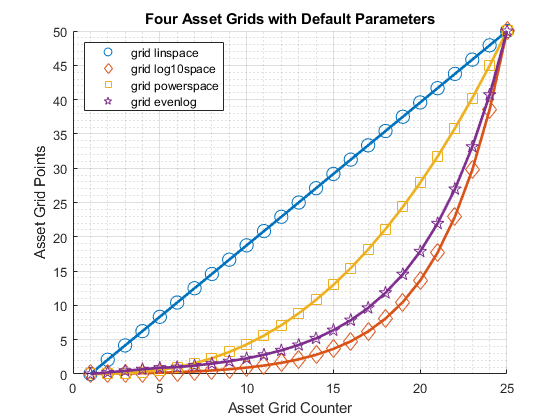
\includegraphics[width=5.20833in,height=\textheight]{img/fx_saveborr_grid_images/figure_0.png}

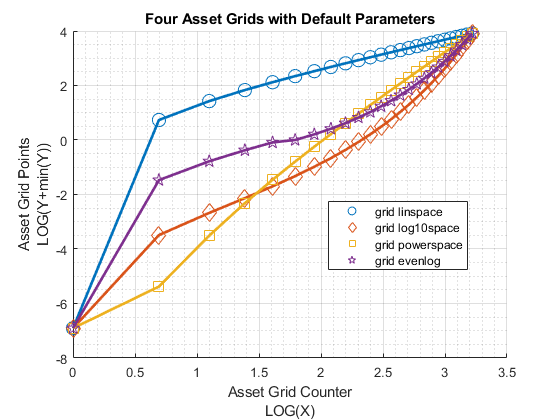
\includegraphics[width=5.20833in,height=\textheight]{img/fx_saveborr_grid_images/figure_1.png}

\hypertarget{test-ff_saveborr_grid-log-grid-changing-parameters}{%
\subsection{Test FF\_SAVEBORR\_GRID Log Grid Changing Parameters}\label{test-ff_saveborr_grid-log-grid-changing-parameters}}

Log grid, same min and max, change log X1 and X2 points

\begin{verbatim}
% Same min and max and grid points
[fl_a_min, fl_a_max, it_a_points] = deal(0,50,25);
st_grid_type = 'grid_log10space';
% Four types of grid points
mp_grid_control = containers.Map('KeyType','char', 'ValueType','any');
mp_grid_control('grid_log10space_x1') = 0.1;
mp_grid_control('grid_log10space_x2') = 1;
[ar_fl_log10space_a] = ff_saveborr_grid(fl_a_min, fl_a_max, it_a_points, st_grid_type, mp_grid_control);
mp_grid_control('grid_log10space_x1') = 0.1/2;
mp_grid_control('grid_log10space_x2') = 1*2;
[ar_fl_log10space_b] = ff_saveborr_grid(fl_a_min, fl_a_max, it_a_points, st_grid_type, mp_grid_control);
mp_grid_control('grid_log10space_x1') = 0.1/4;
mp_grid_control('grid_log10space_x2') = 1*4;
[ar_fl_log10space_c] = ff_saveborr_grid(fl_a_min, fl_a_max, it_a_points, st_grid_type, mp_grid_control);
mp_grid_control('grid_log10space_x1') = 0.1/6;
mp_grid_control('grid_log10space_x2') = 1*6;
[ar_fl_log10space_d] = ff_saveborr_grid(fl_a_min, fl_a_max, it_a_points, st_grid_type, mp_grid_control);
% draw four types of lines jointly
mt_value = [ar_fl_log10space_a'; ar_fl_log10space_b'; ...
    ar_fl_log10space_c'; ar_fl_log10space_d'];
ar_row_grid = [...
    "log10space:x1=0.1/1, x2=1", ...
    "log10space:x1=0.1/2, x2=2", ...
    "log10space:x1=0.1/4, x2=3", ...
    "log10space:x1=0.1/6, x2=4"];
ar_col_grid = 1:it_a_points;
mp_support_graph = containers.Map('KeyType', 'char', 'ValueType', 'any');
mp_support_graph('cl_st_graph_title') = {'Asset Grids with Log 10 Grid Varying Controls'};
mp_support_graph('cl_st_ytitle') = {'Asset Grid Points'};
mp_support_graph('cl_st_xtitle') = {'Asset Grid Counter'};
mp_support_graph('bl_graph_logy') = true; % do not log
ff_graph_grid(mt_value, ar_row_grid, ar_col_grid, mp_support_graph);
\end{verbatim}

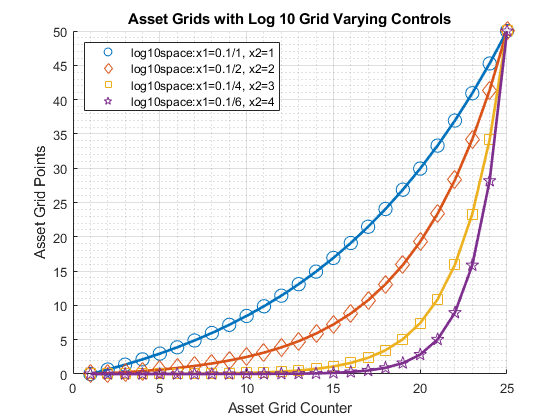
\includegraphics[width=5.20833in,height=\textheight]{img/fx_saveborr_grid_images/figure_2.png}

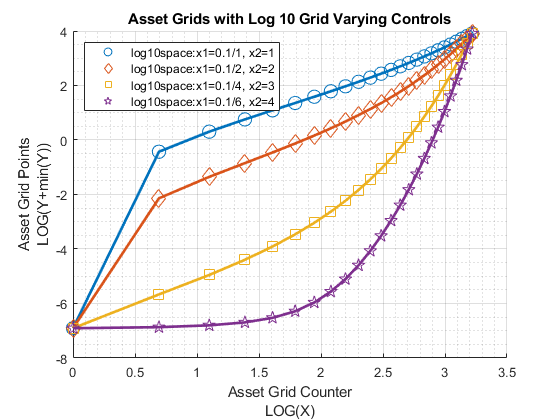
\includegraphics[width=5.20833in,height=\textheight]{img/fx_saveborr_grid_images/figure_3.png}

\hypertarget{test-ff_saveborr_grid-power-grid-changing-parameters}{%
\subsection{Test FF\_SAVEBORR\_GRID Power Grid Changing Parameters}\label{test-ff_saveborr_grid-power-grid-changing-parameters}}

Log grid, same min and max, change log X1 and X2 points

\begin{verbatim}
% Same min and max and grid points
[fl_a_min, fl_a_max, it_a_points] = deal(0,50,25);
st_grid_type = 'grid_powerspace';
% Four types of grid points
mp_grid_control = containers.Map('KeyType','char', 'ValueType','any');
mp_grid_control('grid_powerspace_power') = 1;
[ar_fl_powerspace_a] = ff_saveborr_grid(fl_a_min, fl_a_max, it_a_points, st_grid_type, mp_grid_control);
mp_grid_control('grid_powerspace_power') = 2;
[ar_fl_powerspace_b] = ff_saveborr_grid(fl_a_min, fl_a_max, it_a_points, st_grid_type, mp_grid_control);
mp_grid_control('grid_powerspace_power') = 4;
[ar_fl_powerspace_c] = ff_saveborr_grid(fl_a_min, fl_a_max, it_a_points, st_grid_type, mp_grid_control);
mp_grid_control('grid_powerspace_power') = 6;
[ar_fl_powerspace_d] = ff_saveborr_grid(fl_a_min, fl_a_max, it_a_points, st_grid_type, mp_grid_control);
% draw four types of lines jointly
mt_value = [ar_fl_powerspace_a'; ar_fl_powerspace_b'; ...
    ar_fl_powerspace_c'; ar_fl_powerspace_d'];
ar_row_grid = [...
    "powerspace:power=1", ...
    "powerspace:power=2", ...
    "powerspace:power=4", ...
    "powerspace:power=6"];
ar_col_grid = 1:it_a_points;
mp_support_graph = containers.Map('KeyType', 'char', 'ValueType', 'any');
mp_support_graph('cl_st_graph_title') = {'Asset Grids with Power Grid Varying Controls'};
mp_support_graph('cl_st_ytitle') = {'Asset Grid Points'};
mp_support_graph('cl_st_xtitle') = {'Asset Grid Counter'};
mp_support_graph('bl_graph_logy') = true; % do not log
ff_graph_grid(mt_value, ar_row_grid, ar_col_grid, mp_support_graph);
\end{verbatim}

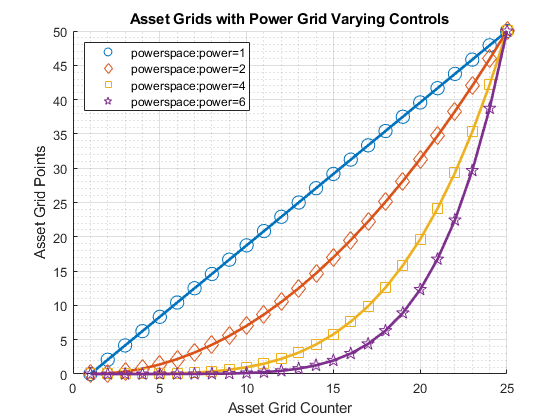
\includegraphics[width=5.20833in,height=\textheight]{img/fx_saveborr_grid_images/figure_4.png}

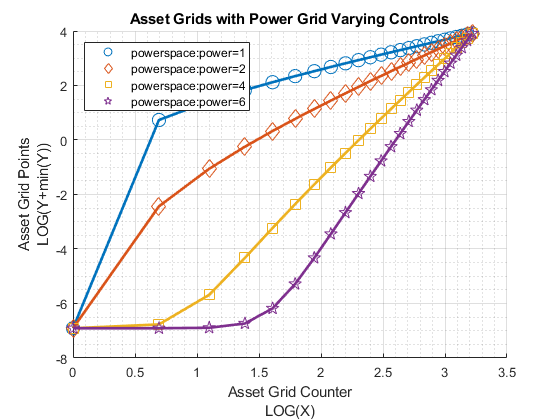
\includegraphics[width=5.20833in,height=\textheight]{img/fx_saveborr_grid_images/figure_5.png}

\hypertarget{test-ff_saveborr_grid-threshold-grid-changing-parameters}{%
\subsection{Test FF\_SAVEBORR\_GRID Threshold Grid Changing Parameters}\label{test-ff_saveborr_grid-threshold-grid-changing-parameters}}

Threshold Grid, Changing Threshold Levels. Initial segments below
threshold are linspace, then logspace.

\begin{verbatim}
% Same min and max and grid points
[fl_a_min, fl_a_max, it_a_points] = deal(0,50,25);
st_grid_type = 'grid_evenlog';
% Four types of grid points
mp_grid_control = containers.Map('KeyType','char', 'ValueType','any');
mp_grid_control('grid_evenlog_threshold') = 0.50;
[ar_fl_evenlog_a] = ff_saveborr_grid(fl_a_min, fl_a_max, it_a_points, st_grid_type, mp_grid_control);
mp_grid_control('grid_evenlog_threshold') = 1.00;
[ar_fl_evenlog_b] = ff_saveborr_grid(fl_a_min, fl_a_max, it_a_points, st_grid_type, mp_grid_control);
mp_grid_control('grid_evenlog_threshold') = 2;
[ar_fl_evenlog_c] = ff_saveborr_grid(fl_a_min, fl_a_max, it_a_points, st_grid_type, mp_grid_control);
mp_grid_control('grid_evenlog_threshold') = 5;
[ar_fl_evenlog_d] = ff_saveborr_grid(fl_a_min, fl_a_max, it_a_points, st_grid_type, mp_grid_control);
% draw four types of lines jointly
mt_value = [ar_fl_evenlog_a'; ar_fl_evenlog_b'; ...
    ar_fl_evenlog_c'; ar_fl_evenlog_d'];
ar_row_grid = [...
    "evenlog:threshold=0.5", ...
    "evenlog:threshold=1.0", ...
    "evenlog:threshold=2.0", ...
    "evenlog:threshold=5.0"];
ar_col_grid = 1:it_a_points;
mp_support_graph = containers.Map('KeyType', 'char', 'ValueType', 'any');
mp_support_graph('cl_st_graph_title') = {'Asset Grids with Threshold Grid Varying Controls'};
mp_support_graph('cl_st_ytitle') = {'Asset Grid Points'};
mp_support_graph('cl_st_xtitle') = {'Asset Grid Counter'};
mp_support_graph('bl_graph_logy') = true; % do not log
ff_graph_grid(mt_value, ar_row_grid, ar_col_grid, mp_support_graph);
\end{verbatim}

\includegraphics[width=5.20833in,height=\textheight]{img/fx_saveborr_grid_images/figure_6.png}

\includegraphics[width=5.20833in,height=\textheight]{img/fx_saveborr_grid_images/figure_7.png}

\hypertarget{common-functions}{%
\chapter{Common Functions}\label{common-functions}}

\hypertarget{ffy_tauchen-ar1-shock-discretization-example}{%
\section{FFY\_TAUCHEN AR1 Shock Discretization Example}\label{ffy_tauchen-ar1-shock-discretization-example}}

\begin{quote}
Go back to \href{http://fanwangecon.github.io/}{fan}'s \href{https://fanwangecon.github.io/MEconTools/}{MEconTools} Toolbox (\href{https://fanwangecon.github.io/MEconTools/bookdown}{bookdown}), \href{https://fanwangecon.github.io/M4Econ/}{Matlab Code Examples} Repository (\href{https://fanwangecon.github.io/M4Econ/bookdown}{bookdown}), or \href{https://fanwangecon.github.io/Math4Econ/}{Math for Econ with Matlab} Repository (\href{https://fanwangecon.github.io/Math4Econ/bookdown}{bookdown}).
\end{quote}

This is the example vignette for function:
\href{https://github.com/FanWangEcon/MEconTools/blob/master/MEconTools/external/stats/ffy_tauchen.m}{\textbf{ffy\_tauchen}}
from the \href{https://fanwangecon.github.io/MEconTools/}{\textbf{MEconTools
Package}}\textbf{.} : See also
the
\href{https://github.com/FanWangEcon/MEconTools/blob/master/MEconTools/external/stats/ffy_rouwenhorst.m}{\textbf{ffy\_rouwenhorst}}
function from the \href{https://fanwangecon.github.io/MEconTools/}{\textbf{MEconTools
Package}}\textbf{.} This function
discretize a mean zero AR1 process, uses Tauchen (1986). See \href{https://fanwangecon.github.io/M4Econ/panel/timeseries/htmlpdfm/fs_autoregressive.html}{AR 1
Example}
for some details on how the AR1 process works. And See \href{https://doi.org/10.1016/j.red.2010.02.002}{Kopecky and Suen
(2010)}.

\hypertarget{test-ffy_tauchen-defaults}{%
\subsection{Test FFY\_TAUCHEN Defaults}\label{test-ffy_tauchen-defaults}}

Call the function with defaults. Default sd bounds arer plus and minus
4. This is used in the following examples, unless otherwise specified as
the 5th parameter.

\begin{verbatim}
ffy_tauchen();

----------------------------------------
xxxxxxxxxxxxxxxxxxxxxxxxxxxxxxxxxxxxxxxx
CONTAINER NAME: mp_container_map ND Array (Matrix etc)
xxxxxxxxxxxxxxxxxxxxxxxxxxxxxxxxxxxxxxxx
                         i    idx    ndim    numel    rowN    colN    sum    mean      std      coefvari       min         max  
                         _    ___    ____    _____    ____    ____    ___    ____    _______    ________    __________    ______

    ar_disc_ar1          1     1      2        5       5       1       0       0     0.79057        Inf             -1         1
    mt_disc_ar1_trans    2     6      2       25       5       5       5     0.2     0.27623     1.3812     7.3923e-12    0.7887

xxx TABLE:ar_disc_ar1 xxxxxxxxxxxxxxxxxx
           c1 
          ____

    r1      -1
    r2    -0.5
    r3       0
    r4     0.5
    r5       1

xxx TABLE:mt_disc_ar1_trans xxxxxxxxxxxxxxxxxx
              c1            c2           c3           c4            c5    
          __________    __________    ________    __________    __________

    r1       0.22663       0.73331    0.040048    1.0689e-05    7.3923e-12
    r2      0.012224       0.58648     0.39831     0.0029797     7.605e-08
    r3    8.8417e-05       0.10556      0.7887       0.10556    8.8417e-05
    r4     7.605e-08     0.0029797     0.39831       0.58648      0.012224
    r5    7.3923e-12    1.0689e-05    0.040048       0.73331       0.22663

----------------------------------------
xxxxxxxxxxxxxxxxxxxxxxxxxxxxxxxxxxxxxxxx
CONTAINER NAME: mp_container_map Scalars
xxxxxxxxxxxxxxxxxxxxxxxxxxxxxxxxxxxxxxxx
                          i    idx    value
                          _    ___    _____

    fl_ar1_persistence    1     2      0.6 
    fl_ar1_step           2     3      0.5 
    fl_shk_std            3     4      0.2 
    it_std_bound          4     5        4 
\end{verbatim}

\hypertarget{test-ffy_tauchen-specify-parameters}{%
\subsection{Test FFY\_TAUCHEN Specify Parameters}\label{test-ffy_tauchen-specify-parameters}}

With a grid of 10 points, the sd bounds on Tauchen and Rouwenhorst are
identical. With the not extremely persistent shock process here, the
Tauchen and Rouwenhorst Results are very similar.

\begin{verbatim}
[fl_ar1_persistence, fl_shk_std, it_disc_points, bl_verbose, it_std_bound] = ...
    deal(0.60, 0.10, 10, true, 3);
ffy_tauchen(fl_ar1_persistence, fl_shk_std, it_disc_points, bl_verbose, it_std_bound);

----------------------------------------
xxxxxxxxxxxxxxxxxxxxxxxxxxxxxxxxxxxxxxxx
CONTAINER NAME: mp_container_map ND Array (Matrix etc)
xxxxxxxxxxxxxxxxxxxxxxxxxxxxxxxxxxxxxxxx
                         i    idx    ndim    numel    rowN    colN        sum           mean          std       coefvari         min          max  
                         _    ___    ____    _____    ____    ____    ___________    ___________    _______    ___________    __________    _______

    ar_disc_ar1          1     1      2        10      10       1     -7.2164e-16    -7.2164e-17     0.2523    -3.4962e+15        -0.375      0.375
    mt_disc_ar1_trans    2     6      2       100      10      10              10            0.1    0.11456         1.1456    1.1798e-08    0.32308

xxx TABLE:ar_disc_ar1 xxxxxxxxxxxxxxxxxx
              c1    
           _________

    r1        -0.375
    r2      -0.29167
    r3      -0.20833
    r4        -0.125
    r5     -0.041667
    r6      0.041667
    r7         0.125
    r8       0.20833
    r9       0.29167
    r10        0.375

xxx TABLE:mt_disc_ar1_trans xxxxxxxxxxxxxxxxxx
               c1            c2            c3            c4           c5          c6           c7            c8            c9           c10    
           __________    __________    __________    __________    ________    ________    __________    __________    __________    __________

    r1        0.13933       0.26196       0.31887       0.20154    0.066066    0.011201    0.00097859    4.3874e-05    1.0053e-06    1.1798e-08
    r2       0.056673       0.16995       0.30658       0.28713      0.1396    0.035167     0.0045756    0.00030628    1.0503e-05    1.8543e-07
    r3        0.01861      0.087039       0.23281       0.32308     0.23281    0.087039      0.016841     0.0016806    8.6129e-05    2.2881e-06
    r4      0.0048925      0.035167        0.1396       0.28713     0.30658     0.16995      0.048841     0.0072547    0.00055483    2.2197e-05
    r5      0.0010235      0.011201      0.066066       0.20154     0.31887     0.26196       0.11169       0.02466     0.0028101    0.00016962
    r6     0.00016962     0.0028101       0.02466       0.11169     0.26196     0.31887       0.20154      0.066066      0.011201     0.0010235
    r7     2.2197e-05    0.00055483     0.0072547      0.048841     0.16995     0.30658       0.28713        0.1396      0.035167     0.0048925
    r8     2.2881e-06    8.6129e-05     0.0016806      0.016841    0.087039     0.23281       0.32308       0.23281      0.087039       0.01861
    r9     1.8543e-07    1.0503e-05    0.00030628     0.0045756    0.035167      0.1396       0.28713       0.30658       0.16995      0.056673
    r10    1.1798e-08    1.0053e-06    4.3874e-05    0.00097859    0.011201    0.066066       0.20154       0.31887       0.26196       0.13933

----------------------------------------
xxxxxxxxxxxxxxxxxxxxxxxxxxxxxxxxxxxxxxxx
CONTAINER NAME: mp_container_map Scalars
xxxxxxxxxxxxxxxxxxxxxxxxxxxxxxxxxxxxxxxx
                          i    idx     value  
                          _    ___    ________

    fl_ar1_persistence    1     2          0.6
    fl_ar1_step           2     3     0.083333
    fl_shk_std            3     4          0.1
    it_std_bound          4     5            3
\end{verbatim}

\hypertarget{test-ffy_tauchen-high-persistence-low-sd}{%
\subsection{Test FFY\_TAUCHEN High Persistence, Low SD}\label{test-ffy_tauchen-high-persistence-low-sd}}

\begin{verbatim}
[fl_ar1_persistence, fl_shk_std, it_disc_points, bl_verbose] = ...
    deal(0.99, 0.01, 7, true);
ffy_tauchen(fl_ar1_persistence, fl_shk_std, it_disc_points, bl_verbose);

----------------------------------------
xxxxxxxxxxxxxxxxxxxxxxxxxxxxxxxxxxxxxxxx
CONTAINER NAME: mp_container_map ND Array (Matrix etc)
xxxxxxxxxxxxxxxxxxxxxxxxxxxxxxxxxxxxxxxx
                         i    idx    ndim    numel    rowN    colN        sum           mean          std       coefvari        min         max  
                         _    ___    ____    _____    ____    ____    ___________    ___________    _______    ___________    ________    _______

    ar_disc_ar1          1     1      2        7       7       1      -5.5511e-17    -7.9302e-18    0.20418    -2.5747e+16    -0.28355    0.28355
    mt_disc_ar1_trans    2     6      2       49       7       7                7        0.14286    0.35355         2.4749           0          1

xxx TABLE:ar_disc_ar1 xxxxxxxxxxxxxxxxxx
              c1     
          ___________

    r1       -0.28355
    r2       -0.18903
    r3      -0.094517
    r4    -2.7756e-17
    r5       0.094517
    r6        0.18903
    r7        0.28355

xxx TABLE:mt_disc_ar1_trans xxxxxxxxxxxxxxxxxx
              c1             c2             c3             c4             c5            c6            c7    
          ___________    ___________    ___________    ___________    __________    __________    __________

    r1              1     4.4497e-06              0              0             0             0             0
    r2     4.4412e-07              1     2.8552e-06              0             0             0             0
    r3      1.632e-46     7.1638e-07              1     1.8164e-06             0             0             0
    r4    9.6185e-124     6.3021e-46     1.1456e-06              1    1.1456e-06             0             0
    r5    6.3206e-239    8.9712e-123     2.4121e-45     1.8164e-06             1    7.1638e-07             0
    r6              0     1.426e-237    8.2932e-122     9.1503e-45    2.8552e-06             1    4.4412e-07
    r7              0              0    3.1885e-236    7.5984e-121    3.4405e-44    4.4497e-06             1

----------------------------------------
xxxxxxxxxxxxxxxxxxxxxxxxxxxxxxxxxxxxxxxx
CONTAINER NAME: mp_container_map Scalars
xxxxxxxxxxxxxxxxxxxxxxxxxxxxxxxxxxxxxxxx
                          i    idx     value  
                          _    ___    ________

    fl_ar1_persistence    1     2         0.99
    fl_ar1_step           2     3     0.094517
    fl_shk_std            3     4         0.01
    it_std_bound          4     5            4
\end{verbatim}

\hypertarget{test-ffy_tauchen-low-persistence-low-sd}{%
\subsection{Test FFY\_TAUCHEN Low Persistence, Low SD}\label{test-ffy_tauchen-low-persistence-low-sd}}

\begin{verbatim}
[fl_ar1_persistence, fl_shk_std, it_disc_points, bl_verbose] = ...
    deal(0.01, 0.01, 7, true);
ffy_tauchen(fl_ar1_persistence, fl_shk_std, it_disc_points, bl_verbose);

----------------------------------------
xxxxxxxxxxxxxxxxxxxxxxxxxxxxxxxxxxxxxxxx
CONTAINER NAME: mp_container_map ND Array (Matrix etc)
xxxxxxxxxxxxxxxxxxxxxxxxxxxxxxxxxxxxxxxx
                         i    idx    ndim    numel    rowN    colN    sum     mean        std       coefvari       min          max   
                         _    ___    ____    _____    ____    ____    ___    _______    ________    ________    __________    ________

    ar_disc_ar1          1     1      2        7       7       1       0           0    0.028805        Inf      -0.040002    0.040002
    mt_disc_ar1_trans    2     6      2       49       7       7       7     0.14286     0.17448     1.2213     0.00037109     0.49504

xxx TABLE:ar_disc_ar1 xxxxxxxxxxxxxxxxxx
             c1    
          _________

    r1    -0.040002
    r2    -0.026668
    r3    -0.013334
    r4            0
    r5     0.013334
    r6     0.026668
    r7     0.040002

xxx TABLE:mt_disc_ar1_trans xxxxxxxxxxxxxxxxxx
              c1           c2         c3         c4         c5          c6           c7    
          __________    ________    _______    _______    _______    ________    __________

    r1    0.00049475    0.024497    0.24044     0.4947    0.21921    0.020299    0.00037109
    r2    0.00047179    0.023751    0.23685    0.49488     0.2227    0.020954    0.00038948
    r3    0.00044982    0.023024    0.23329      0.495    0.22621    0.021626     0.0004087
    r4     0.0004288    0.022316    0.22974    0.49504    0.22974    0.022316     0.0004288
    r5     0.0004087    0.021626    0.22621      0.495    0.23329    0.023024    0.00044982
    r6    0.00038948    0.020954     0.2227    0.49488    0.23685    0.023751    0.00047179
    r7    0.00037109    0.020299    0.21921     0.4947    0.24044    0.024497    0.00049475

----------------------------------------
xxxxxxxxxxxxxxxxxxxxxxxxxxxxxxxxxxxxxxxx
CONTAINER NAME: mp_container_map Scalars
xxxxxxxxxxxxxxxxxxxxxxxxxxxxxxxxxxxxxxxx
                          i    idx     value  
                          _    ___    ________

    fl_ar1_persistence    1     2         0.01
    fl_ar1_step           2     3     0.013334
    fl_shk_std            3     4         0.01
    it_std_bound          4     5            4
\end{verbatim}

\hypertarget{test-ffy_tauchen-high-persistence-high-sd}{%
\subsection{Test FFY\_TAUCHEN High Persistence, High SD}\label{test-ffy_tauchen-high-persistence-high-sd}}

\begin{verbatim}
[fl_ar1_persistence, fl_shk_std, it_disc_points, bl_verbose] = ...
    deal(0.99, 0.99, 7, true);
ffy_tauchen(fl_ar1_persistence, fl_shk_std, it_disc_points, bl_verbose);

----------------------------------------
xxxxxxxxxxxxxxxxxxxxxxxxxxxxxxxxxxxxxxxx
CONTAINER NAME: mp_container_map ND Array (Matrix etc)
xxxxxxxxxxxxxxxxxxxxxxxxxxxxxxxxxxxxxxxx
                         i    idx    ndim    numel    rowN    colN        sum           mean          std       coefvari        min       max  
                         _    ___    ____    _____    ____    ____    ___________    ___________    _______    ___________    _______    ______

    ar_disc_ar1          1     1      2        7       7       1      -3.5527e-15    -5.0753e-16     20.214    -3.9828e+16    -28.072    28.072
    mt_disc_ar1_trans    2     6      2       49       7       7                7        0.14286    0.35355         2.4749          0         1

xxx TABLE:ar_disc_ar1 xxxxxxxxxxxxxxxxxx
            c1   
          _______

    r1    -28.072
    r2    -18.714
    r3    -9.3572
    r4          0
    r5     9.3572
    r6     18.714
    r7     28.072

xxx TABLE:mt_disc_ar1_trans xxxxxxxxxxxxxxxxxx
              c1             c2             c3             c4             c5            c6            c7    
          ___________    ___________    ___________    ___________    __________    __________    __________

    r1              1     4.4497e-06              0              0             0             0             0
    r2     4.4412e-07              1     2.8552e-06              0             0             0             0
    r3      1.632e-46     7.1638e-07              1     1.8164e-06             0             0             0
    r4    9.6185e-124     6.3021e-46     1.1456e-06              1    1.1456e-06             0             0
    r5    6.3206e-239    8.9712e-123     2.4121e-45     1.8164e-06             1    7.1638e-07             0
    r6              0     1.426e-237    8.2932e-122     9.1503e-45    2.8552e-06             1    4.4412e-07
    r7              0              0    3.1885e-236    7.5984e-121    3.4405e-44    4.4497e-06             1

----------------------------------------
xxxxxxxxxxxxxxxxxxxxxxxxxxxxxxxxxxxxxxxx
CONTAINER NAME: mp_container_map Scalars
xxxxxxxxxxxxxxxxxxxxxxxxxxxxxxxxxxxxxxxx
                          i    idx    value 
                          _    ___    ______

    fl_ar1_persistence    1     2       0.99
    fl_ar1_step           2     3     9.3572
    fl_shk_std            3     4       0.99
    it_std_bound          4     5          4
\end{verbatim}

\hypertarget{test-ffy_tauchen-low-persistence-low-sd-1}{%
\subsection{Test FFY\_TAUCHEN Low Persistence, Low SD}\label{test-ffy_tauchen-low-persistence-low-sd-1}}

\begin{verbatim}
[fl_ar1_persistence, fl_shk_std, it_disc_points, bl_verbose] = ...
    deal(0.01, 0.01, 7, true);
ffy_tauchen(fl_ar1_persistence, fl_shk_std, it_disc_points, bl_verbose);

----------------------------------------
xxxxxxxxxxxxxxxxxxxxxxxxxxxxxxxxxxxxxxxx
CONTAINER NAME: mp_container_map ND Array (Matrix etc)
xxxxxxxxxxxxxxxxxxxxxxxxxxxxxxxxxxxxxxxx
                         i    idx    ndim    numel    rowN    colN    sum     mean        std       coefvari       min          max   
                         _    ___    ____    _____    ____    ____    ___    _______    ________    ________    __________    ________

    ar_disc_ar1          1     1      2        7       7       1       0           0    0.028805        Inf      -0.040002    0.040002
    mt_disc_ar1_trans    2     6      2       49       7       7       7     0.14286     0.17448     1.2213     0.00037109     0.49504

xxx TABLE:ar_disc_ar1 xxxxxxxxxxxxxxxxxx
             c1    
          _________

    r1    -0.040002
    r2    -0.026668
    r3    -0.013334
    r4            0
    r5     0.013334
    r6     0.026668
    r7     0.040002

xxx TABLE:mt_disc_ar1_trans xxxxxxxxxxxxxxxxxx
              c1           c2         c3         c4         c5          c6           c7    
          __________    ________    _______    _______    _______    ________    __________

    r1    0.00049475    0.024497    0.24044     0.4947    0.21921    0.020299    0.00037109
    r2    0.00047179    0.023751    0.23685    0.49488     0.2227    0.020954    0.00038948
    r3    0.00044982    0.023024    0.23329      0.495    0.22621    0.021626     0.0004087
    r4     0.0004288    0.022316    0.22974    0.49504    0.22974    0.022316     0.0004288
    r5     0.0004087    0.021626    0.22621      0.495    0.23329    0.023024    0.00044982
    r6    0.00038948    0.020954     0.2227    0.49488    0.23685    0.023751    0.00047179
    r7    0.00037109    0.020299    0.21921     0.4947    0.24044    0.024497    0.00049475

----------------------------------------
xxxxxxxxxxxxxxxxxxxxxxxxxxxxxxxxxxxxxxxx
CONTAINER NAME: mp_container_map Scalars
xxxxxxxxxxxxxxxxxxxxxxxxxxxxxxxxxxxxxxxx
                          i    idx     value  
                          _    ___    ________

    fl_ar1_persistence    1     2         0.01
    fl_ar1_step           2     3     0.013334
    fl_shk_std            3     4         0.01
    it_std_bound          4     5            4
\end{verbatim}

\hypertarget{ffy_rouwenhorst-ar1-shock-discretization-example}{%
\section{FFY\_ROUWENHORST AR1 Shock Discretization Example}\label{ffy_rouwenhorst-ar1-shock-discretization-example}}

\begin{quote}
Go back to \href{http://fanwangecon.github.io/}{fan}'s \href{https://fanwangecon.github.io/MEconTools/}{MEconTools} Toolbox (\href{https://fanwangecon.github.io/MEconTools/bookdown}{bookdown}), \href{https://fanwangecon.github.io/M4Econ/}{Matlab Code Examples} Repository (\href{https://fanwangecon.github.io/M4Econ/bookdown}{bookdown}), or \href{https://fanwangecon.github.io/Math4Econ/}{Math for Econ with Matlab} Repository (\href{https://fanwangecon.github.io/Math4Econ/bookdown}{bookdown}).
\end{quote}

This is the example vignette for function:
\href{https://github.com/FanWangEcon/MEconTools/blob/master/MEconTools/external/stats/ffy_rouwenhorst.m}{\textbf{ffy\_rouwenhorst}}
from the \href{https://fanwangecon.github.io/MEconTools/}{\textbf{MEconTools
Package}}\textbf{.} See also
\href{https://github.com/FanWangEcon/MEconTools/blob/master/MEconTools/external/stats/ffy_tauchen.m}{\textbf{ffy\_tauchen}}
function from the \href{https://fanwangecon.github.io/MEconTools/}{\textbf{MEconTools
Package}}\textbf{.} This function
discretize a mean zero AR1 process, uses Rouwenhorst (1995). See \href{https://fanwangecon.github.io/M4Econ/panel/timeseries/htmlpdfm/fs_autoregressive.html}{AR 1
Example}
for some details on how the AR1 process works. And See \href{https://doi.org/10.1016/j.red.2010.02.002}{Kopecky and Suen
(2010)}.

\hypertarget{test-ffy_rouwenhorst-defaults}{%
\subsection{Test FFY\_ROUWENHORST Defaults}\label{test-ffy_rouwenhorst-defaults}}

Call the function with defaults.

\begin{verbatim}
ffy_rouwenhorst();

----------------------------------------
xxxxxxxxxxxxxxxxxxxxxxxxxxxxxxxxxxxxxxxx
CONTAINER NAME: mp_container_map ND Array (Matrix etc)
xxxxxxxxxxxxxxxxxxxxxxxxxxxxxxxxxxxxxxxx
                         i    idx    ndim    numel    rowN    colN    sum    mean      std      coefvari     min       max  
                         _    ___    ____    _____    ____    ____    ___    ____    _______    ________    ______    ______

    ar_disc_ar1          1     1      2        5       5       1       0       0     0.39528        Inf       -0.5       0.5
    mt_disc_ar1_trans    2    11      2       25       5       5       5     0.2     0.18246    0.91229     0.0016    0.5136

xxx TABLE:ar_disc_ar1 xxxxxxxxxxxxxxxxxx
           c1  
          _____

    r1     -0.5
    r2    -0.25
    r3        0
    r4     0.25
    r5      0.5

xxx TABLE:mt_disc_ar1_trans xxxxxxxxxxxxxxxxxx
            c1        c2        c3        c4        c5  
          ______    ______    ______    ______    ______

    r1    0.4096    0.4096    0.1536    0.0256    0.0016
    r2    0.1024    0.4864    0.3264    0.0784    0.0064
    r3    0.0256    0.2176    0.5136    0.2176    0.0256
    r4    0.0064    0.0784    0.3264    0.4864    0.1024
    r5    0.0016    0.0256    0.1536    0.4096    0.4096

----------------------------------------
xxxxxxxxxxxxxxxxxxxxxxxxxxxxxxxxxxxxxxxx
CONTAINER NAME: mp_container_map Scalars
xxxxxxxxxxxxxxxxxxxxxxxxxxxxxxxxxxxxxxxx
                          i    idx    value
                          _    ___    _____

    fl_ar1_beg            1     2     -0.5 
    fl_ar1_end            2     3      0.5 
    fl_ar1_persistence    3     4      0.6 
    fl_ar1_step           4     5     0.25 
    fl_p0                 5     6      0.8 
    fl_q0                 6     7      0.8 
    fl_shk_std            7     8      0.2 
    fl_sig_ar1            8     9     0.25 
    it_std_bound          9    10        0 
\end{verbatim}

\hypertarget{test-ffy_rouwenhorst-specify-parameters}{%
\subsection{Test FFY\_ROUWENHORST Specify Parameters}\label{test-ffy_rouwenhorst-specify-parameters}}

With a grid of 10 points, the Rwouenhorst bounds on standard deviations
are equall to Tauchen bounds of 3. With the not extremely persistent
shock process here, the Tauchen and Rouwenhorst Results are very
similar.

\begin{verbatim}
[fl_ar1_persistence, fl_shk_std, it_disc_points, bl_verbose] = ...
    deal(0.60, 0.10, 10, true);
ffy_rouwenhorst(fl_ar1_persistence, fl_shk_std, it_disc_points, bl_verbose);

----------------------------------------
xxxxxxxxxxxxxxxxxxxxxxxxxxxxxxxxxxxxxxxx
CONTAINER NAME: mp_container_map ND Array (Matrix etc)
xxxxxxxxxxxxxxxxxxxxxxxxxxxxxxxxxxxxxxxx
                         i    idx    ndim    numel    rowN    colN       sum           mean         std       coefvari       min         max  
                         _    ___    ____    _____    ____    ____    __________    __________    _______    __________    ________    _______

    ar_disc_ar1          1     1      2        10      10       1     5.5511e-17    5.5511e-18     0.2523    4.5451e+16      -0.375      0.375
    mt_disc_ar1_trans    2    11      2       100      10      10             10           0.1    0.11724        1.1724    5.12e-07    0.33477

xxx TABLE:ar_disc_ar1 xxxxxxxxxxxxxxxxxx
              c1    
           _________

    r1        -0.375
    r2      -0.29167
    r3      -0.20833
    r4        -0.125
    r5     -0.041667
    r6      0.041667
    r7         0.125
    r8       0.20833
    r9       0.29167
    r10        0.375

xxx TABLE:mt_disc_ar1_trans xxxxxxxxxxxxxxxxxx
               c1            c2            c3           c4           c5          c6          c7            c8            c9           c10    
           __________    __________    __________    _________    ________    ________    _________    __________    __________    __________

    r1        0.13422       0.30199       0.30199      0.17616     0.06606    0.016515    0.0027525    0.00029491    1.8432e-05      5.12e-07
    r2       0.033554       0.20133       0.32716      0.26424     0.12662    0.038535    0.0075694    0.00093389    6.6048e-05     2.048e-06
    r3      0.0083886      0.081789       0.26267      0.32755     0.21401    0.082747     0.019741     0.0028677    0.00023347     8.192e-06
    r4      0.0020972      0.028312       0.14038      0.30946     0.30369     0.15877     0.047989     0.0084603    0.00081101    3.2768e-05
    r5     0.00052429      0.009044      0.061145      0.20246     0.33477     0.25969      0.10585      0.023642     0.0027525    0.00013107
    r6     0.00013107     0.0027525      0.023642      0.10585     0.25969     0.33477      0.20246      0.061145      0.009044    0.00052429
    r7     3.2768e-05    0.00081101     0.0084603     0.047989     0.15877     0.30369      0.30946       0.14038      0.028312     0.0020972
    r8      8.192e-06    0.00023347     0.0028677     0.019741    0.082747     0.21401      0.32755       0.26267      0.081789     0.0083886
    r9      2.048e-06    6.6048e-05    0.00093389    0.0075694    0.038535     0.12662      0.26424       0.32716       0.20133      0.033554
    r10      5.12e-07    1.8432e-05    0.00029491    0.0027525    0.016515     0.06606      0.17616       0.30199       0.30199       0.13422

----------------------------------------
xxxxxxxxxxxxxxxxxxxxxxxxxxxxxxxxxxxxxxxx
CONTAINER NAME: mp_container_map Scalars
xxxxxxxxxxxxxxxxxxxxxxxxxxxxxxxxxxxxxxxx
                          i    idx     value  
                          _    ___    ________

    fl_ar1_beg            1     2       -0.375
    fl_ar1_end            2     3        0.375
    fl_ar1_persistence    3     4          0.6
    fl_ar1_step           4     5     0.083333
    fl_p0                 5     6          0.8
    fl_q0                 6     7          0.8
    fl_shk_std            7     8          0.1
    fl_sig_ar1            8     9        0.125
    it_std_bound          9    10            0
\end{verbatim}

\hypertarget{test-ffy_rouwenhorst-high-persistence-low-sd}{%
\subsection{Test FFY\_ROUWENHORST High Persistence, Low SD}\label{test-ffy_rouwenhorst-high-persistence-low-sd}}

\begin{verbatim}
[fl_ar1_persistence, fl_shk_std, it_disc_points, bl_verbose] = ...
    deal(0.99, 0.01, 7, true);
ffy_rouwenhorst(fl_ar1_persistence, fl_shk_std, it_disc_points, bl_verbose);

----------------------------------------
xxxxxxxxxxxxxxxxxxxxxxxxxxxxxxxxxxxxxxxx
CONTAINER NAME: mp_container_map ND Array (Matrix etc)
xxxxxxxxxxxxxxxxxxxxxxxxxxxxxxxxxxxxxxxx
                         i    idx    ndim    numel    rowN    colN    sum     mean        std      coefvari       min          max  
                         _    ___    ____    _____    ____    ____    ___    _______    _______    ________    __________    _______

    ar_disc_ar1          1     1      2        7       7       1       0           0    0.12503        Inf       -0.17364    0.17364
    mt_disc_ar1_trans    2    11      2       49       7       7       7     0.14286    0.34148     2.3904     1.5625e-14    0.97059

xxx TABLE:ar_disc_ar1 xxxxxxxxxxxxxxxxxx
             c1   
          ________

    r1    -0.17364
    r2    -0.11576
    r3    -0.05788
    r4           0
    r5     0.05788
    r6     0.11576
    r7     0.17364

xxx TABLE:mt_disc_ar1_trans xxxxxxxxxxxxxxxxxx
              c1            c2            c3            c4            c5            c6            c7    
          __________    __________    __________    __________    __________    __________    __________

    r1       0.97037      0.029257    0.00036756    2.4627e-06    9.2815e-09    1.8656e-11    1.5625e-14
    r2     0.0048762        0.9705      0.024382    0.00024504    1.2314e-06    3.0938e-09    3.1094e-12
    r3    2.4504e-05      0.009753       0.97057      0.019506    0.00014703    4.9254e-07    6.1877e-10
    r4    1.2313e-07    7.3513e-05       0.01463       0.97059       0.01463    7.3513e-05    1.2313e-07
    r5    6.1877e-10    4.9254e-07    0.00014703      0.019506       0.97057      0.009753    2.4504e-05
    r6    3.1094e-12    3.0938e-09    1.2314e-06    0.00024504      0.024382        0.9705     0.0048762
    r7    1.5625e-14    1.8656e-11    9.2815e-09    2.4627e-06    0.00036756      0.029257       0.97037

----------------------------------------
xxxxxxxxxxxxxxxxxxxxxxxxxxxxxxxxxxxxxxxx
CONTAINER NAME: mp_container_map Scalars
xxxxxxxxxxxxxxxxxxxxxxxxxxxxxxxxxxxxxxxx
                          i    idx     value  
                          _    ___    ________

    fl_ar1_beg            1     2     -0.17364
    fl_ar1_end            2     3      0.17364
    fl_ar1_persistence    3     4         0.99
    fl_ar1_step           4     5      0.05788
    fl_p0                 5     6        0.995
    fl_q0                 6     7        0.995
    fl_shk_std            7     8         0.01
    fl_sig_ar1            8     9     0.070888
    it_std_bound          9    10            0
\end{verbatim}

\hypertarget{test-ffy_rouwenhorst-low-persistence-low-sd}{%
\subsection{Test FFY\_ROUWENHORST Low Persistence, Low SD}\label{test-ffy_rouwenhorst-low-persistence-low-sd}}

\begin{verbatim}
[fl_ar1_persistence, fl_shk_std, it_disc_points, bl_verbose] = ...
    deal(0.01, 0.01, 7, true);
ffy_rouwenhorst(fl_ar1_persistence, fl_shk_std, it_disc_points, bl_verbose);

----------------------------------------
xxxxxxxxxxxxxxxxxxxxxxxxxxxxxxxxxxxxxxxx
CONTAINER NAME: mp_container_map ND Array (Matrix etc)
xxxxxxxxxxxxxxxxxxxxxxxxxxxxxxxxxxxxxxxx
                         i    idx    ndim    numel    rowN    colN    sum     mean        std       coefvari       min         max   
                         _    ___    ____    _____    ____    ____    ___    _______    ________    ________    _________    ________

    ar_disc_ar1          1     1      2        7       7       1       0           0    0.017639        Inf     -0.024496    0.024496
    mt_disc_ar1_trans    2    11      2       49       7       7       7     0.14286     0.10985    0.76893      0.014711     0.31252

xxx TABLE:ar_disc_ar1 xxxxxxxxxxxxxxxxxx
              c1    
          __________

    r1     -0.024496
    r2     -0.016331
    r3    -0.0081654
    r4             0
    r5     0.0081654
    r6      0.016331
    r7      0.024496

xxx TABLE:mt_disc_ar1_trans xxxxxxxxxxxxxxxxxx
             c1          c2         c3         c4         c5          c6          c7   
          ________    ________    _______    _______    _______    ________    ________

    r1    0.016586    0.097547    0.23904    0.31241    0.22966    0.090047    0.014711
    r2    0.016258    0.096266    0.23749    0.31247    0.23124    0.091266    0.015008
    r3    0.015936    0.094997    0.23594    0.31251    0.23281    0.092497    0.015311
    r4     0.01562    0.093741    0.23438    0.31252    0.23438    0.093741     0.01562
    r5    0.015311    0.092497    0.23281    0.31251    0.23594    0.094997    0.015936
    r6    0.015008    0.091266    0.23124    0.31247    0.23749    0.096266    0.016258
    r7    0.014711    0.090047    0.22966    0.31241    0.23904    0.097547    0.016586

----------------------------------------
xxxxxxxxxxxxxxxxxxxxxxxxxxxxxxxxxxxxxxxx
CONTAINER NAME: mp_container_map Scalars
xxxxxxxxxxxxxxxxxxxxxxxxxxxxxxxxxxxxxxxx
                          i    idx      value  
                          _    ___    _________

    fl_ar1_beg            1     2     -0.024496
    fl_ar1_end            2     3      0.024496
    fl_ar1_persistence    3     4          0.01
    fl_ar1_step           4     5     0.0081654
    fl_p0                 5     6         0.505
    fl_q0                 6     7         0.505
    fl_shk_std            7     8          0.01
    fl_sig_ar1            8     9      0.010001
    it_std_bound          9    10             0
\end{verbatim}

\hypertarget{test-ffy_rouwenhorst-high-persistence-high-sd}{%
\subsection{Test FFY\_ROUWENHORST High Persistence, High SD}\label{test-ffy_rouwenhorst-high-persistence-high-sd}}

\begin{verbatim}
[fl_ar1_persistence, fl_shk_std, it_disc_points, bl_verbose] = ...
    deal(0.99, 0.99, 7, true);
ffy_rouwenhorst(fl_ar1_persistence, fl_shk_std, it_disc_points, bl_verbose);

----------------------------------------
xxxxxxxxxxxxxxxxxxxxxxxxxxxxxxxxxxxxxxxx
CONTAINER NAME: mp_container_map ND Array (Matrix etc)
xxxxxxxxxxxxxxxxxxxxxxxxxxxxxxxxxxxxxxxx
                         i    idx    ndim    numel    rowN    colN       sum           mean         std      coefvari        min          max  
                         _    ___    ____    _____    ____    ____    __________    __________    _______    _________    __________    _______

    ar_disc_ar1          1     1      2        7       7       1      3.5527e-15    5.0753e-16     12.378    2.439e+16        -17.19      17.19
    mt_disc_ar1_trans    2    11      2       49       7       7               7       0.14286    0.34148       2.3904    1.5625e-14    0.97059

xxx TABLE:ar_disc_ar1 xxxxxxxxxxxxxxxxxx
            c1   
          _______

    r1     -17.19
    r2     -11.46
    r3    -5.7301
    r4          0
    r5     5.7301
    r6      11.46
    r7      17.19

xxx TABLE:mt_disc_ar1_trans xxxxxxxxxxxxxxxxxx
              c1            c2            c3            c4            c5            c6            c7    
          __________    __________    __________    __________    __________    __________    __________

    r1       0.97037      0.029257    0.00036756    2.4627e-06    9.2815e-09    1.8656e-11    1.5625e-14
    r2     0.0048762        0.9705      0.024382    0.00024504    1.2314e-06    3.0938e-09    3.1094e-12
    r3    2.4504e-05      0.009753       0.97057      0.019506    0.00014703    4.9254e-07    6.1877e-10
    r4    1.2313e-07    7.3513e-05       0.01463       0.97059       0.01463    7.3513e-05    1.2313e-07
    r5    6.1877e-10    4.9254e-07    0.00014703      0.019506       0.97057      0.009753    2.4504e-05
    r6    3.1094e-12    3.0938e-09    1.2314e-06    0.00024504      0.024382        0.9705     0.0048762
    r7    1.5625e-14    1.8656e-11    9.2815e-09    2.4627e-06    0.00036756      0.029257       0.97037

----------------------------------------
xxxxxxxxxxxxxxxxxxxxxxxxxxxxxxxxxxxxxxxx
CONTAINER NAME: mp_container_map Scalars
xxxxxxxxxxxxxxxxxxxxxxxxxxxxxxxxxxxxxxxx
                          i    idx    value 
                          _    ___    ______

    fl_ar1_beg            1     2     -17.19
    fl_ar1_end            2     3      17.19
    fl_ar1_persistence    3     4       0.99
    fl_ar1_step           4     5     5.7301
    fl_p0                 5     6      0.995
    fl_q0                 6     7      0.995
    fl_shk_std            7     8       0.99
    fl_sig_ar1            8     9     7.0179
    it_std_bound          9    10          0
\end{verbatim}

\hypertarget{test-ffy_rouwenhorst-low-persistence-low-sd-1}{%
\subsection{Test FFY\_ROUWENHORST Low Persistence, Low SD}\label{test-ffy_rouwenhorst-low-persistence-low-sd-1}}

\begin{verbatim}
[fl_ar1_persistence, fl_shk_std, it_disc_points, bl_verbose] = ...
    deal(0.01, 0.01, 7, true);
ffy_rouwenhorst(fl_ar1_persistence, fl_shk_std, it_disc_points, bl_verbose);

----------------------------------------
xxxxxxxxxxxxxxxxxxxxxxxxxxxxxxxxxxxxxxxx
CONTAINER NAME: mp_container_map ND Array (Matrix etc)
xxxxxxxxxxxxxxxxxxxxxxxxxxxxxxxxxxxxxxxx
                         i    idx    ndim    numel    rowN    colN    sum     mean        std       coefvari       min         max   
                         _    ___    ____    _____    ____    ____    ___    _______    ________    ________    _________    ________

    ar_disc_ar1          1     1      2        7       7       1       0           0    0.017639        Inf     -0.024496    0.024496
    mt_disc_ar1_trans    2    11      2       49       7       7       7     0.14286     0.10985    0.76893      0.014711     0.31252

xxx TABLE:ar_disc_ar1 xxxxxxxxxxxxxxxxxx
              c1    
          __________

    r1     -0.024496
    r2     -0.016331
    r3    -0.0081654
    r4             0
    r5     0.0081654
    r6      0.016331
    r7      0.024496

xxx TABLE:mt_disc_ar1_trans xxxxxxxxxxxxxxxxxx
             c1          c2         c3         c4         c5          c6          c7   
          ________    ________    _______    _______    _______    ________    ________

    r1    0.016586    0.097547    0.23904    0.31241    0.22966    0.090047    0.014711
    r2    0.016258    0.096266    0.23749    0.31247    0.23124    0.091266    0.015008
    r3    0.015936    0.094997    0.23594    0.31251    0.23281    0.092497    0.015311
    r4     0.01562    0.093741    0.23438    0.31252    0.23438    0.093741     0.01562
    r5    0.015311    0.092497    0.23281    0.31251    0.23594    0.094997    0.015936
    r6    0.015008    0.091266    0.23124    0.31247    0.23749    0.096266    0.016258
    r7    0.014711    0.090047    0.22966    0.31241    0.23904    0.097547    0.016586

----------------------------------------
xxxxxxxxxxxxxxxxxxxxxxxxxxxxxxxxxxxxxxxx
CONTAINER NAME: mp_container_map Scalars
xxxxxxxxxxxxxxxxxxxxxxxxxxxxxxxxxxxxxxxx
                          i    idx      value  
                          _    ___    _________

    fl_ar1_beg            1     2     -0.024496
    fl_ar1_end            2     3      0.024496
    fl_ar1_persistence    3     4          0.01
    fl_ar1_step           4     5     0.0081654
    fl_p0                 5     6         0.505
    fl_q0                 6     7         0.505
    fl_shk_std            7     8          0.01
    fl_sig_ar1            8     9      0.010001
    it_std_bound          9    10             0
\end{verbatim}

\hypertarget{appendix-appendix}{%
\appendix}


\hypertarget{index-and-code-links}{%
\chapter{Index and Code Links}\label{index-and-code-links}}

\hypertarget{savings-dynamic-programming-links}{%
\section{Savings Dynamic Programming links}\label{savings-dynamic-programming-links}}

\begin{enumerate}
\def\labelenumi{\arabic{enumi}.}
\tightlist
\item
  \href{https://fanwangecon.github.io/MEconTools/MEconTools/doc/vfi/htmlpdfm/fx_vfi_az_loop.html}{Looped Grid Infinite Horizon Dynamic Savings Problem}: \href{https://github.com/FanWangEcon/MEconTools/blob/master/MEconTools/doc/vfi/fx_vfi_az_loop.mlx}{\textbf{mlx}} \textbar{} \href{https://github.com/FanWangEcon/MEconTools/blob/master/MEconTools/doc/vfi/htmlpdfm/fx_vfi_az_loop.m}{\textbf{m}} \textbar{} \href{https://github.com/FanWangEcon/MEconTools/blob/master/MEconTools/doc/vfi/htmlpdfm/fx_vfi_az_loop.pdf}{\textbf{pdf}} \textbar{} \href{https://fanwangecon.github.io/MEconTools/MEconTools/doc/vfi/htmlpdfm/fx_vfi_az_loop.html}{\textbf{html}}

  \begin{itemize}
  \tightlist
  \item
    Common grid looped solution
  \item
    Slow, but easy to modify, useful for developing new models
  \item
    Given preferences, some AR(1) shock process, solve the infinite horizon household savings dynamic programming problem. The state-space and choice-space share the same asset grid.
  \item
    \textbf{MEconTools}: \emph{\href{https://github.com/FanWangEcon/MEconTools/blob/master/MEconTools/vfi/ff_vfi_az_loop.m}{ff\_vfi\_az\_loop()}}
  \end{itemize}
\item
  \href{https://fanwangecon.github.io/MEconTools/MEconTools/doc/vfi/htmlpdfm/fx_vfi_az_vec.html}{Vectorized Grid Infinite Horizon Dynamic Savings Problem}: \href{https://github.com/FanWangEcon/MEconTools/blob/master/MEconTools/doc/vfi/fx_vfi_az_vec.mlx}{\textbf{mlx}} \textbar{} \href{https://github.com/FanWangEcon/MEconTools/blob/master/MEconTools/doc/vfi/htmlpdfm/fx_vfi_az_vec.m}{\textbf{m}} \textbar{} \href{https://github.com/FanWangEcon/MEconTools/blob/master/MEconTools/doc/vfi/htmlpdfm/fx_vfi_az_vec.pdf}{\textbf{pdf}} \textbar{} \href{https://fanwangecon.github.io/MEconTools/MEconTools/doc/vfi/htmlpdfm/fx_vfi_az_vec.html}{\textbf{html}}

  \begin{itemize}
  \tightlist
  \item
    Common grid vectorized solution
  \item
    Fast, sufficiently approximate value(a,z), but c(a,z) not precise
  \item
    Given preferences, some AR(1) shock process, solve the infinite horizon household savings dynamic programming problem. The state-space and choice-space share the same asset grid.
  \item
    \textbf{MEconTools}: \emph{\href{https://github.com/FanWangEcon/MEconTools/blob/master/MEconTools/vfi/ff_vfi_az_vec.m}{ff\_vfi\_az\_vec()}}
  \end{itemize}
\item
  \href{https://fanwangecon.github.io/MEconTools/MEconTools/doc/vfi/htmlpdfm/fx_vfi_az_bisec_loop.html}{Looped Exact Infinite Horizon Dynamic Savings Problem}: \href{https://github.com/FanWangEcon/MEconTools/blob/master/MEconTools/doc/vfi/fx_vfi_az_bisec_loop.mlx}{\textbf{mlx}} \textbar{} \href{https://github.com/FanWangEcon/MEconTools/blob/master/MEconTools/doc/vfi/htmlpdfm/fx_vfi_az_bisec_loop.m}{\textbf{m}} \textbar{} \href{https://github.com/FanWangEcon/MEconTools/blob/master/MEconTools/doc/vfi/htmlpdfm/fx_vfi_az_bisec_loop.pdf}{\textbf{pdf}} \textbar{} \href{https://fanwangecon.github.io/MEconTools/MEconTools/doc/vfi/htmlpdfm/fx_vfi_az_bisec_loop.html}{\textbf{html}}

  \begin{itemize}
  \tightlist
  \item
    Infinite horizon constrained dynamic savings problem with persistent shock.
  \item
    The state-space is on a grid, the choice space are continuous percentages of cash-on-hand.
  \item
    Looped exact savings-percentage algorithm, slow but high precision at low grid size.
  \item
    Solves for EV(ap,z) given shock state and for a savings choice. Bisection based on FOC with analytical du(c(ap))/dap and spline slopes dEV(ap,z)/dap.
  \item
    \textbf{MEconTools}: \emph{\href{https://github.com/FanWangEcon/MEconTools/blob/master/MEconTools/vfi/ff_vfi_az_bisec_loop.m}{ff\_vfi\_az\_bisec\_loop()} + \href{https://github.com/FanWangEcon/MEconTools/blob/master/MEconTools/optim/ff_optim_bisec_savezrone.m}{ff\_optim\_bisec\_savezrone()}}
  \end{itemize}
\item
  \href{https://fanwangecon.github.io/MEconTools/MEconTools/doc/vfi/htmlpdfm/fx_vfi_az_bisec_vec.html}{Vectorized Exact Infinite Horizon Dynamic Savings Problem}: \href{https://github.com/FanWangEcon/MEconTools/blob/master/MEconTools/doc/vfi/fx_vfi_az_bisec_vec.mlx}{\textbf{mlx}} \textbar{} \href{https://github.com/FanWangEcon/MEconTools/blob/master/MEconTools/doc/vfi/htmlpdfm/fx_vfi_az_bisec_vec.m}{\textbf{m}} \textbar{} \href{https://github.com/FanWangEcon/MEconTools/blob/master/MEconTools/doc/vfi/htmlpdfm/fx_vfi_az_bisec_vec.pdf}{\textbf{pdf}} \textbar{} \href{https://fanwangecon.github.io/MEconTools/MEconTools/doc/vfi/htmlpdfm/fx_vfi_az_bisec_vec.html}{\textbf{html}}

  \begin{itemize}
  \tightlist
  \item
    Exact choice vectorized solution
  \item
    Fast, approximates choices with higher precision (given value grid, accurate up to 0.001525878 percent of individual-specific cash-on-hand)
  \item
    Given preferences, some AR(1) shock process, solve the infinite horizon household savings dynamic programming problem. The state-space is on a grid. The choice space are continuous percentages of cash-on-hand.
  \item
    \textbf{MEconTools}: \emph{\href{https://github.com/FanWangEcon/MEconTools/blob/master/MEconTools/vfi/ff_vfi_az_bisec_vec.m}{ff\_vfi\_az\_bisec\_vec()}}
  \end{itemize}
\end{enumerate}

\hypertarget{summarize-policy-and-value-links}{%
\section{Summarize Policy and Value links}\label{summarize-policy-and-value-links}}

\begin{enumerate}
\def\labelenumi{\arabic{enumi}.}
\tightlist
\item
  \href{https://fanwangecon.github.io/MEconTools/MEconTools/doc/summ/htmlpdfm/fx_summ_nd_array.html}{Summarize ND Array Policy and Value Functions}: \href{https://github.com/FanWangEcon/MEconTools/blob/master/MEconTools/doc/summ/fx_summ_nd_array.mlx}{\textbf{mlx}} \textbar{} \href{https://github.com/FanWangEcon/MEconTools/blob/master/MEconTools/doc/summ/htmlpdfm/fx_summ_nd_array.m}{\textbf{m}} \textbar{} \href{https://github.com/FanWangEcon/MEconTools/blob/master/MEconTools/doc/summ/htmlpdfm/fx_summ_nd_array.pdf}{\textbf{pdf}} \textbar{} \href{https://fanwangecon.github.io/MEconTools/MEconTools/doc/summ/htmlpdfm/fx_summ_nd_array.html}{\textbf{html}}

  \begin{itemize}
  \tightlist
  \item
    Given an NDarray matrix with N1, N2, \ldots, ND dimensions. Generate average and standard deviation for the 3rd dimension, grouping by the other dimensions.
  \item
    For example, show the 5th dimension as the column groups, and the other variables generate combinations shown as rows.
  \item
    The resulting summary statistics table contains mean and standard deviation among other statistics over the policy or value contained in the ND array.
  \item
    \textbf{MEconTools}: \emph{ff\_summ\_nd\_array()}
  \end{itemize}
\end{enumerate}

\hypertarget{distributional-analysis-links}{%
\section{Distributional Analysis links}\label{distributional-analysis-links}}

\begin{enumerate}
\def\labelenumi{\arabic{enumi}.}
\tightlist
\item
  \href{https://fanwangecon.github.io/MEconTools/MEconTools/doc/stats/htmlpdfm/fx_simu_stats.html}{Gateway Joint Probability Mass Statistics}: \href{https://github.com/FanWangEcon/MEconTools/blob/master/MEconTools/doc/stats/fx_simu_stats.mlx}{\textbf{mlx}} \textbar{} \href{https://github.com/FanWangEcon/MEconTools/blob/master/MEconTools/doc/stats/htmlpdfm/fx_simu_stats.m}{\textbf{m}} \textbar{} \href{https://github.com/FanWangEcon/MEconTools/blob/master/MEconTools/doc/stats/htmlpdfm/fx_simu_stats.pdf}{\textbf{pdf}} \textbar{} \href{https://fanwangecon.github.io/MEconTools/MEconTools/doc/stats/htmlpdfm/fx_simu_stats.html}{\textbf{html}}

  \begin{itemize}
  \tightlist
  \item
    Given probability mass function f(s), and information y(s), x(s), z(s) at each element of the state-space, compute statistics for each variable, y, x, z, which are all discrete random variables.
  \item
    Compute their correlation and covariance.
  \item
    \textbf{MEconTools}: \emph{ff\_simu\_stats()}
  \end{itemize}
\item
  \href{https://fanwangecon.github.io/MEconTools/MEconTools/doc/stats/htmlpdfm/fx_disc_rand_var_stats.html}{Discrete Random Variable Distributional Statistics}: \href{https://github.com/FanWangEcon/MEconTools/blob/master/MEconTools/doc/stats/fx_disc_rand_var_stats.mlx}{\textbf{mlx}} \textbar{} \href{https://github.com/FanWangEcon/MEconTools/blob/master/MEconTools/doc/stats/htmlpdfm/fx_disc_rand_var_stats.m}{\textbf{m}} \textbar{} \href{https://github.com/FanWangEcon/MEconTools/blob/master/MEconTools/doc/stats/htmlpdfm/fx_disc_rand_var_stats.pdf}{\textbf{pdf}} \textbar{} \href{https://fanwangecon.github.io/MEconTools/MEconTools/doc/stats/htmlpdfm/fx_disc_rand_var_stats.html}{\textbf{html}}

  \begin{itemize}
  \tightlist
  \item
    Model simulation generates discrete random variables, calculate mean, standard deviation, min, max, percentiles, and proportion of outcomes held by x percentiles, etc.
  \item
    \textbf{MEconTools}: \emph{ff\_disc\_rand\_var\_stats()}
  \end{itemize}
\item
  \href{https://fanwangecon.github.io/MEconTools/MEconTools/doc/stats/htmlpdfm/fx_disc_rand_var_mass2outcomes.html}{Generate Discrete Random Variable}: \href{https://github.com/FanWangEcon/MEconTools/blob/master/MEconTools/doc/stats/fx_disc_rand_var_mass2outcomes.mlx}{\textbf{mlx}} \textbar{} \href{https://github.com/FanWangEcon/MEconTools/blob/master/MEconTools/doc/stats/htmlpdfm/fx_disc_rand_var_mass2outcomes.m}{\textbf{m}} \textbar{} \href{https://github.com/FanWangEcon/MEconTools/blob/master/MEconTools/doc/stats/htmlpdfm/fx_disc_rand_var_mass2outcomes.pdf}{\textbf{pdf}} \textbar{} \href{https://fanwangecon.github.io/MEconTools/MEconTools/doc/stats/htmlpdfm/fx_disc_rand_var_mass2outcomes.html}{\textbf{html}}

  \begin{itemize}
  \tightlist
  \item
    Given mass at state space points, and y, c, a, z and other outcomes or other information at each corresponding state space points, generate discrete random variable, with unique sorted values, and mass for each unique sorted values.
  \item
    Generate additional joint distributions: if initial distribution is over f(a,z), generate joint distribution of f(y,a) or f(y,z).
  \item
    \textbf{MEconTools}: \emph{ff\_disc\_rand\_var\_mass2outcomes()}
  \end{itemize}
\item
  \href{https://fanwangecon.github.io/MEconTools/MEconTools/doc/stats/htmlpdfm/fx_disc_rand_var_mass2covcor.html}{Discrete Random Variable Correlation and Covariance}: \href{https://github.com/FanWangEcon/MEconTools/blob/master/MEconTools/doc/stats/fx_disc_rand_var_mass2covcor.mlx}{\textbf{mlx}} \textbar{} \href{https://github.com/FanWangEcon/MEconTools/blob/master/MEconTools/doc/stats/htmlpdfm/fx_disc_rand_var_mass2covcor.m}{\textbf{m}} \textbar{} \href{https://github.com/FanWangEcon/MEconTools/blob/master/MEconTools/doc/stats/htmlpdfm/fx_disc_rand_var_mass2covcor.pdf}{\textbf{pdf}} \textbar{} \href{https://fanwangecon.github.io/MEconTools/MEconTools/doc/stats/htmlpdfm/fx_disc_rand_var_mass2covcor.html}{\textbf{html}}

  \begin{itemize}
  \tightlist
  \item
    Given probability mass function f(s), X(s), and Y(s), compute the covariance and correlation betwen X and Y.
  \item
    \textbf{MEconTools}: \emph{ff\_disc\_rand\_var\_mass2covcor()}
  \end{itemize}
\end{enumerate}

\hypertarget{optimizers-links}{%
\section{Optimizers links}\label{optimizers-links}}

\begin{enumerate}
\def\labelenumi{\arabic{enumi}.}
\tightlist
\item
  \href{https://fanwangecon.github.io/MEconTools/MEconTools/doc/optim/htmlpdfm/fx_optim_bisec_savezrone.html}{Bisection Exact Optimal Savings Share Multiple States}: \href{https://github.com/FanWangEcon/MEconTools/blob/master/MEconTools/doc/optim/fx_optim_bisec_savezrone.mlx}{\textbf{mlx}} \textbar{} \href{https://github.com/FanWangEcon/MEconTools/blob/master/MEconTools/doc/optim/htmlpdfm/fx_optim_bisec_savezrone.m}{\textbf{m}} \textbar{} \href{https://github.com/FanWangEcon/MEconTools/blob/master/MEconTools/doc/optim/htmlpdfm/fx_optim_bisec_savezrone.pdf}{\textbf{pdf}} \textbar{} \href{https://fanwangecon.github.io/MEconTools/MEconTools/doc/optim/htmlpdfm/fx_optim_bisec_savezrone.html}{\textbf{html}}

  \begin{itemize}
  \tightlist
  \item
    Given a First Order Condition function handle that takes the fraction of resources (cash-on-hand) saved as the input, solve for the optimal savings fraction via bisection. Solve this concurrently for many elements of the state-space. The function handle contains the FOC with parameters and state-space elements embeded.
  \item
    \textbf{MEconTools}: \emph{\href{https://github.com/FanWangEcon/MEconTools/blob/master/MEconTools/optim/ff_optim_bisec_savezrone.m}{ff\_optim\_bisec\_savezrone()}}
  \end{itemize}
\item
  \href{https://fanwangecon.github.io/MEconTools/MEconTools/doc/optim/htmlpdfm/fx_optim_mlsec_savezrone.html}{Multisection Exact Optimal Savings Share Multiple States}: \href{https://github.com/FanWangEcon/MEconTools/blob/master/MEconTools/doc/optim/fx_optim_mlsec_savezrone.mlx}{\textbf{mlx}} \textbar{} \href{https://github.com/FanWangEcon/MEconTools/blob/master/MEconTools/doc/optim/htmlpdfm/fx_optim_mlsec_savezrone.m}{\textbf{m}} \textbar{} \href{https://github.com/FanWangEcon/MEconTools/blob/master/MEconTools/doc/optim/htmlpdfm/fx_optim_mlsec_savezrone.pdf}{\textbf{pdf}} \textbar{} \href{https://fanwangecon.github.io/MEconTools/MEconTools/doc/optim/htmlpdfm/fx_optim_mlsec_savezrone.html}{\textbf{html}}

  \begin{itemize}
  \tightlist
  \item
    Given a First Order Condition function handle that takes the fraction of resources (cash-on-hand) saved as the input, solve for the optimal savings fraction via multisection where there are multiple evaluations per iteration of the FOC. Solve this concurrently for many elements of the state-space. The function handle contains the FOC with parameters and state-space elements embeded.
  \item
    \textbf{MEconTools}: \emph{\href{https://github.com/FanWangEcon/MEconTools/blob/master/MEconTools/optim/ff_optim_mlsec_savezrone.m}{ff\_optim\_mlsec\_savezrone()}}
  \end{itemize}
\item
  \href{https://fanwangecon.github.io/MEconTools/MEconTools/doc/optim/htmlpdfm/fx_optim_mzoom_savezrone.html}{Vectorized Zooming Exact Optimal Savings Share Multiple States}: \href{https://github.com/FanWangEcon/MEconTools/blob/master/MEconTools/doc/optim/fx_optim_mzoom_savezrone.mlx}{\textbf{mlx}} \textbar{} \href{https://github.com/FanWangEcon/MEconTools/blob/master/MEconTools/doc/optim/htmlpdfm/fx_optim_mzoom_savezrone.m}{\textbf{m}} \textbar{} \href{https://github.com/FanWangEcon/MEconTools/blob/master/MEconTools/doc/optim/htmlpdfm/fx_optim_mzoom_savezrone.pdf}{\textbf{pdf}} \textbar{} \href{https://fanwangecon.github.io/MEconTools/MEconTools/doc/optim/htmlpdfm/fx_optim_mzoom_savezrone.html}{\textbf{html}}

  \begin{itemize}
  \tightlist
  \item
    Given a Utility (not FOC) function handle that takes the fraction of resources (cash-on-hand) saved as the input, solve for the optimal savings fraction via iterative zooming where there are multiple evaluations per iteration of the utility function. Solve this concurrently for many elements of the state-space. The function handle contains the utilty function with parameters and state-space elements embeded.
  \item
    \textbf{MEconTools}: \emph{\href{https://github.com/FanWangEcon/MEconTools/blob/master/MEconTools/optim/ff_optim_mzoom_savezrone.m}{ff\_optim\_mzoom\_savezrone()}}
  \end{itemize}
\end{enumerate}

\hypertarget{graphs-links}{%
\section{Graphs links}\label{graphs-links}}

\begin{enumerate}
\def\labelenumi{\arabic{enumi}.}
\tightlist
\item
  \href{https://fanwangecon.github.io/MEconTools/MEconTools/doc/graph/htmlpdfm/fx_graph_grid.html}{Multiple Line Graph Function}: \href{https://github.com/FanWangEcon/MEconTools/blob/master/MEconTools/doc/graph/fx_graph_grid.mlx}{\textbf{mlx}} \textbar{} \href{https://github.com/FanWangEcon/MEconTools/blob/master/MEconTools/doc/graph/htmlpdfm/fx_graph_grid.m}{\textbf{m}} \textbar{} \href{https://github.com/FanWangEcon/MEconTools/blob/master/MEconTools/doc/graph/htmlpdfm/fx_graph_grid.pdf}{\textbf{pdf}} \textbar{} \href{https://fanwangecon.github.io/MEconTools/MEconTools/doc/graph/htmlpdfm/fx_graph_grid.html}{\textbf{html}}

  \begin{itemize}
  \tightlist
  \item
    Grid based Graph, x-axis one param, color another param, over outcomes.
  \item
    \textbf{MEconTools}: \emph{ff\_graph\_grid()}
  \end{itemize}
\end{enumerate}

\hypertarget{support-tools-links}{%
\section{Support Tools links}\label{support-tools-links}}

\begin{enumerate}
\def\labelenumi{\arabic{enumi}.}
\tightlist
\item
  \href{https://fanwangecon.github.io/MEconTools/MEconTools/doc/tools/htmlpdfm/fx_container_map_display.html}{Organizes and Prints Container Map Key and Values}: \href{https://github.com/FanWangEcon/MEconTools/blob/master/MEconTools/doc/tools/fx_container_map_display.mlx}{\textbf{mlx}} \textbar{} \href{https://github.com/FanWangEcon/MEconTools/blob/master/MEconTools/doc/tools/htmlpdfm/fx_container_map_display.m}{\textbf{m}} \textbar{} \href{https://github.com/FanWangEcon/MEconTools/blob/master/MEconTools/doc/tools/htmlpdfm/fx_container_map_display.pdf}{\textbf{pdf}} \textbar{} \href{https://fanwangecon.github.io/MEconTools/MEconTools/doc/tools/htmlpdfm/fx_container_map_display.html}{\textbf{html}}

  \begin{itemize}
  \tightlist
  \item
    Summarizes the contents of a map container by data types. Includes, scalar, array, matrix, string, functions, tensors (3-tuples), tesseracts (4-tuples).
  \item
    \textbf{MEconTools}: \emph{ff\_container\_map\_display()}
  \end{itemize}
\end{enumerate}

\hypertarget{data-structures-links}{%
\section{Data Structures links}\label{data-structures-links}}

\begin{enumerate}
\def\labelenumi{\arabic{enumi}.}
\tightlist
\item
  \href{https://fanwangecon.github.io/MEconTools/MEconTools/doc/generate/htmlpdfm/fx_saveborr_grid.html}{Log and Power Spaced Asset and Choice Grids}: \href{https://github.com/FanWangEcon/MEconTools/blob/master/MEconTools/doc/generate/fx_saveborr_grid.mlx}{\textbf{mlx}} \textbar{} \href{https://github.com/FanWangEcon/MEconTools/blob/master/MEconTools/doc/generate/htmlpdfm/fx_saveborr_grid.m}{\textbf{m}} \textbar{} \href{https://github.com/FanWangEcon/MEconTools/blob/master/MEconTools/doc/generate/htmlpdfm/fx_saveborr_grid.pdf}{\textbf{pdf}} \textbar{} \href{https://fanwangecon.github.io/MEconTools/MEconTools/doc/generate/htmlpdfm/fx_saveborr_grid.html}{\textbf{html}}

  \begin{itemize}
  \tightlist
  \item
    Generate linear, log-space, power-space, or threshold-cut asset or choice grids.
  \item
    \textbf{MEconTools}: \emph{ff\_saveborr\_grid()}
  \end{itemize}
\end{enumerate}

\hypertarget{common-functions-links}{%
\section{Common Functions links}\label{common-functions-links}}

\begin{enumerate}
\def\labelenumi{\arabic{enumi}.}
\tightlist
\item
  \href{https://fanwangecon.github.io/MEconTools/MEconTools/doc/external/htmlpdfm/fxy_tauchen.html}{Discretize AR1 Normal Shock Tauchen (1986)}: \href{https://github.com/FanWangEcon/MEconTools/blob/master/MEconTools/doc/external/fxy_tauchen.mlx}{\textbf{mlx}} \textbar{} \href{https://github.com/FanWangEcon/MEconTools/blob/master/MEconTools/doc/external/htmlpdfm/fxy_tauchen.m}{\textbf{m}} \textbar{} \href{https://github.com/FanWangEcon/MEconTools/blob/master/MEconTools/doc/external/htmlpdfm/fxy_tauchen.pdf}{\textbf{pdf}} \textbar{} \href{https://fanwangecon.github.io/MEconTools/MEconTools/doc/external/htmlpdfm/fxy_tauchen.html}{\textbf{html}}

  \begin{itemize}
  \tightlist
  \item
    Mean zero AR(1) shock discretize following Tauchen (1986).
  \item
    \textbf{MEconTools}: \emph{ffy\_tauchen()}
  \end{itemize}
\item
  \href{https://fanwangecon.github.io/MEconTools/MEconTools/doc/external/htmlpdfm/fxy_rouwenhorst.html}{Discretize AR1 Normal Shock Rouwenhorst (1995)}: \href{https://github.com/FanWangEcon/MEconTools/blob/master/MEconTools/doc/external/fxy_rouwenhorst.mlx}{\textbf{mlx}} \textbar{} \href{https://github.com/FanWangEcon/MEconTools/blob/master/MEconTools/doc/external/htmlpdfm/fxy_rouwenhorst.m}{\textbf{m}} \textbar{} \href{https://github.com/FanWangEcon/MEconTools/blob/master/MEconTools/doc/external/htmlpdfm/fxy_rouwenhorst.pdf}{\textbf{pdf}} \textbar{} \href{https://fanwangecon.github.io/MEconTools/MEconTools/doc/external/htmlpdfm/fxy_rouwenhorst.html}{\textbf{html}}

  \begin{itemize}
  \tightlist
  \item
    Mean zero AR(1) shock discretize following Rouwenhorst (1995).
  \item
    \textbf{MEconTools}: \emph{ffy\_rouwenhorst()}
  \end{itemize}
\end{enumerate}

  \bibliography{book.bib,packages.bib}

\end{document}
